\begin{filecontents}{leer.eps}
%!PS-Adobe-2.0 EPSF-2.0
%%CreationDate: Mon Jul 13 16:51:17 1992
%%DocumentFonts: (atend)
%%Pages: 0 1
%%BoundingBox: 72 31 601 342
%%EndComments

gsave
72 31 moveto
72 342 lineto
601 342 lineto
601 31 lineto
72 31 lineto
showpage
grestore
%%Trailer
%%DocumentFonts: Helvetica
\end{filecontents}
%
%\documentclass[epj]{svjour}
\documentclass[epj,referee]{svjour}
% Remove option referee for final version
%
%\usepackage{latexsym}
\usepackage{graphics}
\usepackage{url}

\newcommand{\unit}[1]{\ensuremath{\, \mathrm{#1}}}
\newcommand{\nuc}[2]{$^{#1}$#2}
\newcommand{\reac}[2]{($#1$,$#2$)}
\newcommand{\dr}{DRAGON}
\newcommand{\EcmM}[1]{$E_\mathrm{c.m.} = #1 \unit{MeV}$}
\newcommand{\Ecmk}[1]{$E_\mathrm{c.m.} = #1 \unit{keV}$}
\setcounter{tocdepth}{2}
\newcommand{\pgamma}[4]{$^{#1}$#2($p,\gamma$)$^{#3}$#4}
\newcommand{\agamma}[4]{$^{#1}$#2($\alpha,\gamma$)$^{#3}$#4}


\begin{document}
%
%\title{Radiative capture reactions in inverse kinematics for nuclear astrophysics}
\title{Recoil separators for radiative capture using radioactive ion beams}
\subtitle{Recent advances and detection techniques}
\author{ Chris Ruiz\inst{1} \thanks{\emph{Corresponding author:}email address \texttt{ruiz@triumf.ca}} \and Uwe Greife\inst{2} \and Ulrike Hager\inst{2} }%                     % Do not remove
%
%
\institute{TRIUMF, 4004 Wesbrook Mall, Vancouver, BC, Canada \and Colorado School of Mines, Golden, CO, USA}
%
\date{Received: date / Revised version: date}
% The correct dates will be entered by Springer
%
\abstract{
Radiative capture reactions involving the fusion of hydrogen or helium are ubiquitous in the stellar history of the universe, and are some of the most important reactions in the processes that govern nucleosynthesis and energy generation in both static and explosive scenarios. However, radiative capture reactions pose some of the most difficult measurements challenges due to extremely small cross sections. With the advent of recoil separators and techniques in inverse kinematics, it is now possible to measure radiative capture reactions on very short-lived radioactive nuclei, and in the presence of high experimental backgrounds. In this paper we review the experimental needs for making measurements of astrophysical importance on radiative capture reactions. We also review some of the important historical advances in the field of recoil separators as well as describe current techniques and performance milestones, including descriptions of some of the separators most recently working at radioactive ion beam facilities, such as DRAGON at TRIUMF and the DRS at the Holifield Radioactive Ion Beam Facility. We will also summarize some of the scientific highlight measurements at the RIB facilities.   
\PACS{
      {29.30.Aj}{Charged-particle spectrometers: electric and magnetic} \and
      {29.38.-c}{Radioactive beams} \and
      {25.40.Lw}{Radiative capture}   \and
      {25.40.Ny}{Resonance reactions}
    } 
}


\maketitle

\tableofcontents

\section{Introduction}
\label{intro}

Due to the high abundance of hydrogen left over from the Big Bang, most stellar environments involve proton induced reactions, which produce energy or contribute to the nucleosynthesis of heavier elements via the rapid proton (rp) process that can occur in situations of high temperature and density. In addition, helium is the second most abundant chemical species in the universe, originating in primordial nucleosynthesis and stellar hydrogen burning. This in turn drives the further development of stars through helium burning in the red giant phase and bridges important nucleosynthesis network gaps in the onset of the rp-process. Among the proton and alpha particle induced reactions a very important class is the {\em radiative capture reactions}, defined as those two-body fusion reactions in which the compound nucleus emits one or more $\gamma$ rays (or in rare cases additional e$^{+}$-e$^{-}$ pairs) and is left residing in its ground or metastable state, without the intermediate emission of hadrons. 

These radiative capture reactions may proceed via a {\em resonant} process, in which individual excited states in the compound nucleus give rise to a large enhancement in the reaction cross section; {\em direct capture} involving a process analogous to {\em bremsstrahlung}; or {\em continuum capture}, where many closely-spaced levels contribute. At the typical peak temperatures found in static and explosive stellar scenarios, the properties of nuclei are such that the radiative capture cross sections are vanishingly small\footnote{in general radiative capture cross sections between charged particles are small because of the value of the fine structure constant, i.e. the relative weakness of the electromagnetic interaction compared to the strong interaction.}, making the reactions extremely challenging to measure using the levels of accelerated beam intensity and techniques that are currently in existence. 

Nevertheless, over the last few decades great progress has been made in measuring, calculating and tabulating the radiative capture reactions that contribute to static and explosive stellar scenarios and are vital inputs to our astrophysical models.  For static burning scenarios the relevant reactions were last compiled by the European NACRE effort \cite{angu99}, while the relevance of specific reactions in explosive scenarios was investigated in {\it e.g.} Schatz {\it et al.} \cite{scha98} and Iliadis {\it et al.} \cite{ilia02}. A series of proton-capture thermonuclear reaction rates for A = 20 -- 40 nuclei was also tabulated in Iliadis {\it et al.} \cite{ilia01}, based on updated information from nuclear experiments and statistical model calculations. 
An evaluation of rates which considered the most recent experimental and theoretical inputs was presented in the body of work by Longland and Iliadis \cite{Lon10,Ili10a,Ili10b,Ili10c}.
 %\cite{Lon10}\cite{Ili10a}\cite{Ili10b}\cite{Ili10c}.
Prior to all these works many of the rates used in astrophysical network calculations were from the tabulation of Caughlan \& Fowler \cite{caug88}. Many reaction rates of importance remain unmeasured or uncertain however.

In quiescent stellar burning, radiative capture reactions involving light nuclei tend to be of importance: examples are the \pgamma{7}{Be}{8}{B} reaction, for its role in determining the solar neutrino flux, or the \agamma{12}{C}{16}{O} reaction, for determining the carbon-oxygen ratio in the cores of red giants. In addition, radiative capture reactions are important members of the CNO cycles. 
In higher temperature scenarios such as ``hot-bottom burning" in AGB stars, radiative capture on heavier nuclei can become relevant in determining the nucleosynthetic products of those environments. 
In classical novae, reactions on CNO nuclei and heavier seed material can involve radiative capture reactions up to the $A=40$ region, and of special importance are those within the hot-CNO, Ne-Na-Mg and Mg-Al cycles. In type I X-ray bursts, the rp-process can involve radiative proton- and alpha-capture reactions all the way up to the Sn-Te region. 
Radiative capture reactions are also prolific in the explosions underlying type-Ia and type-II supernovae, as well as playing a role in the {\em p-process}, thought to contribute to the formation of the neutron-deficient p-nuclei from  $^{76}$Se to $^{196}$Hg. In essence, there are very few astrophysical burning or explosion scenarios in which radiative capture reactions between charged particles are of {\em minor} importance.   

With increase of temperature in the astrophysical environment, radiative capture reactions on radioactive isotopes become relatively more important. This naturally leads to a higher degree of experimental complexity due to the need of handling the active materials and increased backgrounds that show up in the radiation detectors employed. Traditionally, with easier availability of light proton and alpha beams from low energy accelerators, radiative capture experiments for nuclear astrophysics were performed in `normal' kinematics with the light ion beam striking a usually solid target. The limitations encountered with this approach are mainly due to cosmic ray, natural terrestrial activity, and/or beam induced background in the detectors used for the measurement of radiative capture $\gamma$ radiation. For this reason the inverse kinematics approach was developed which originally just reduced some of the beam induced background problems. However, it also allowed the use of radioactive ion beams covering the regime of short-lived isotopes, some with half-lives less than a few seconds. While the measurement of radiative capture reactions with the normal kinematics approach is taken to the extremes in the existing (LUNA I+II) and proposed (LUNA III \& DIANA) underground accelerator laboratories, the inverse kinematics method employing recoil separators is used or proposed for all present and future radioactive ion beam facilities. This report tries to summarize the approach, its technical features and successes up to this point in time.


\subsection{Role of radiative capture in stellar environments}
\label{role}

A radiative capture reaction is that in which any nucleus $^{A_{1}}_{Z_{1}}X$ fuses with another $^{A_{2}}_{Z_{2}}Y$ to form a product nucleus $^{A_{1}+A_{2}}_{Z_{1}+Z_{2}}C$, with the emission of $\gamma$ rays. Since the present paper deals almost exclusively with proton and alpha capture reactions, we will continue the illustration with the example of proton capture, so that the radiative capture reaction would be written as
\begin{equation}
^{A}_{Z}T+p\Rightarrow^{A+1}_{Z+1}C+\sum_{i}^{N}{\gamma_{i}}
\end{equation}
where $^{A}_{Z}T$ is the target nucleus. The standard nuclear physics notation for such a reaction would be $^{A}_{Z}T$(p,$\gamma$)$^{A+1}_{Z+1}C$, or rather target(projectile,$\gamma$)recoil. It is sometimes common in nuclear physics experiments for the notation to reflect the laboratory kinematics of the reaction, so that the previous expression would denote a proton impinging on a stationary target nucleus $^{A}_{Z}T$, while in {\it inverse} kinematics, where the proton is stationary and the large nucleus is moving the notation would be $p(^{A}_{Z}T,\gamma)^{A+1}_{Z+1}C$. However since most discussion in the astrophysical context involves the centre-of-mass system of the two particles, the normal kinematics notation will be adopted as universal throughout this paper. 

In the fusion of a proton with a nucleus, the total energy in the centre-of-mass system is given by $m(^{A}_{Z}T)+m(p)+E$, where $m(^{A}_{Z}T)$ and $m(p)$ are the masses\footnote{Usually atomic masses are used in the calculation of inverse kinematics properties, since the target atom resides in its nuclear ground state and neutral atomic state, while the beam ion will exist in a certain charge state $q$. Thus the actual mass of the beam ion as a fraction of the atomic species will be $M_{ion}/M_{atom}=1-\frac{(Z-q)0.511}{A(931.494)+\Delta(^{A}_{Z}X)}$. For typical values of atomic and mass number $Z,A$, mass excess $\Delta$, this results in ion masses  on the order of 99.9\% of the atomic mass. This results in kinetic energy changes small enough to be neglected.} of the target nucleus and the proton respectively (in {\em natural units} where $c=1$) and $E$ is the relative kinetic energy in the centre-of-mass. The final state of the system will be the product nucleus $^{A+1}_{Z+1}C$ in its ground state, with a total emitted $\gamma$-ray energy $E_{\gamma}$ (in the c.m. system), so that
\begin{equation}
E_{\gamma}=E+m(^{A}_{Z}T)+m(p)-m(^{A+1}_{Z+1}C)=E+Q
\end{equation}
where $Q$ is the reaction $Q$-value, and is equal to the proton separation energy of the compound nucleus. Thus the higher the $Q$-value or the higher the particles' relative velocity, the more energy is released in the form of $\gamma$ rays in these reactions. 
 
As one moves away from the line of stability in the direction of decreasing neutron number, nuclear binding energies decrease. This means that proton separation energies are smaller than at the line of stability. This is particularly relevant for static and explosive hydrogen burning, since in these cases, the fusion of protons or alpha particles with such nuclei off the line of stability is usually governed by a combination of direct capture and/or a few isolated, narrow resonances corresponding to relatively low-lying states in the compound nucleus. As a result the reaction rate is extremely sensitive to temperature, i.e. the distribution of particle collision energies. In general, as temperature is increased, more resonances at higher collision energies are involved, increasing the reaction cross section and allowing the radiative capture to occur more frequently. In contrast, the ($p$,$\gamma$) reactions going on very close to the line of stability will access areas in the compound nucleus with higher level density, because of the larger reaction $Q$-values. As one increases in collision energy the states accessed will eventually become alpha-unbound, leading to the preference of ($p$,$\alpha$) reactions over ($p$,$\gamma$). In such cases quasi-cycles are formed such as the CNO, hot-CNO, Ne-Na and Mg-Al cycles (e.g. figs \ref{fig:hotCNO} and \ref{fig:NeNa}). In order to then break out of these cycles it is left to the ($p$,$\gamma$) reactions slightly further from stability, involving short-lived radioactive nuclei (or in the case of the hot-CNO cycle ($\alpha$,$\gamma$) reactions and other charged-particle reactions). In contrast, in situations of very high temperature, the level densities accessed in the compound nucleus can be quite high. In those cases a suitable statistical approach like the Hauser-Feschbach \cite{Hau52} formalism can be applied to calculate radiative capture rates.  

\begin{figure}
\centering
\resizebox{1.0\columnwidth}{!}{
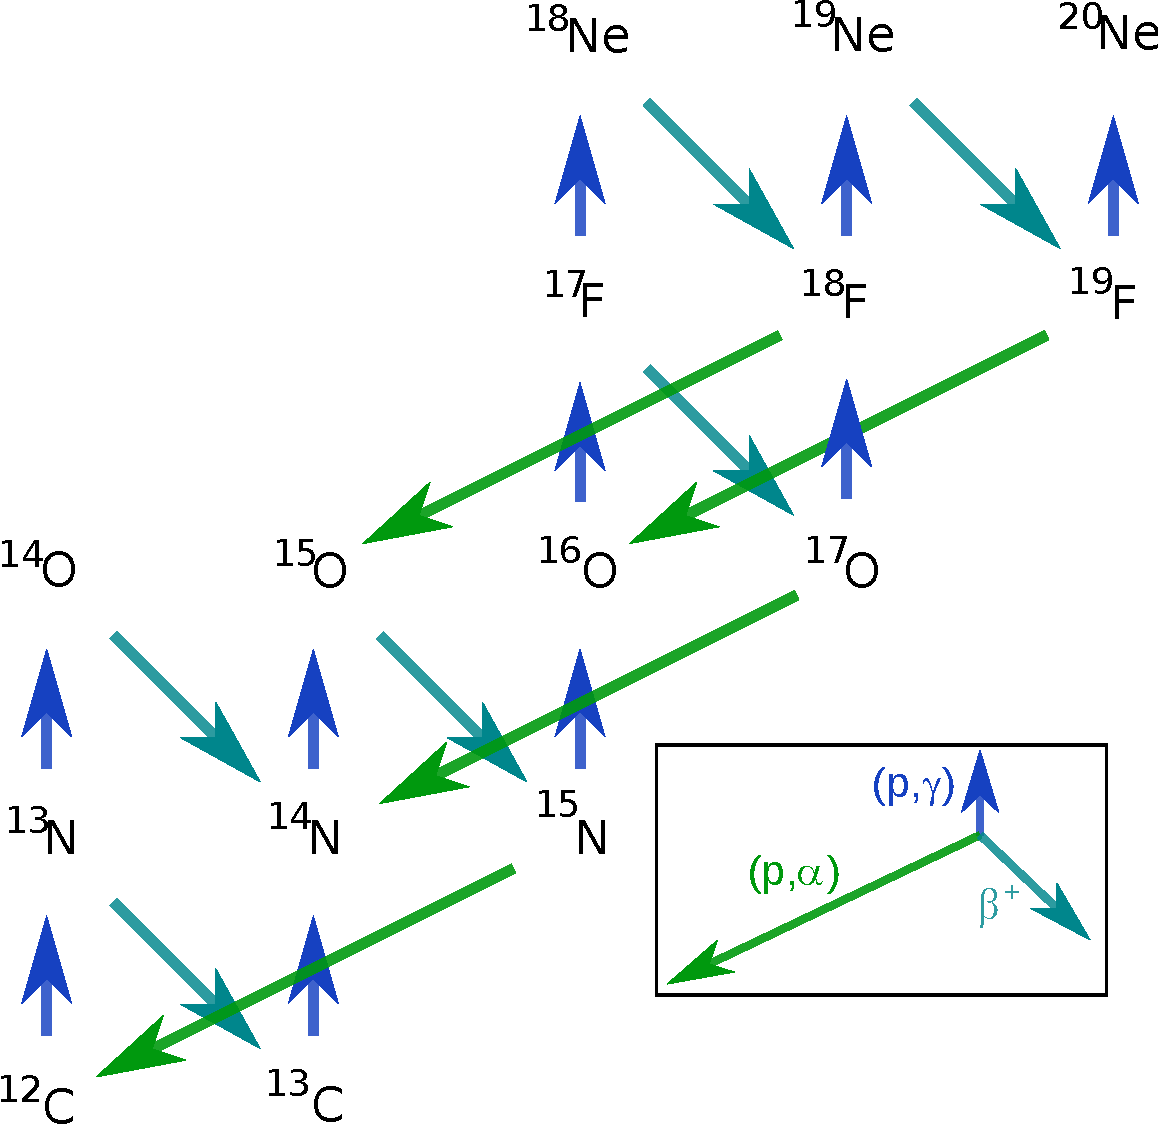
\includegraphics{HotCNO_general.pdf}
}
\caption{The hot CNO cycle.}
\label{fig:hotCNO}
\end{figure}
%
%
\begin{figure}
\centering
\resizebox{0.7\columnwidth}{!}{
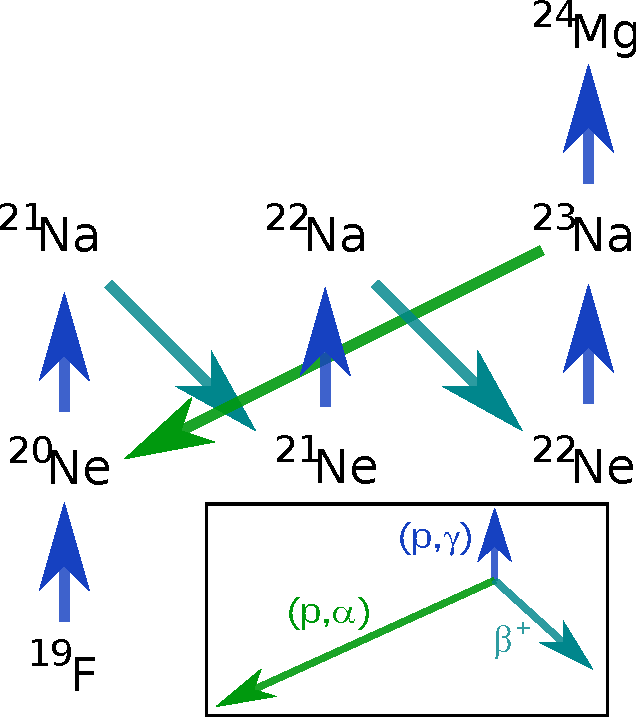
\includegraphics{NeNa-cycle_legend.pdf}
}
\caption{The Ne-Na cycle.}
\label{fig:NeNa}
\end{figure}
%

The proton- and alpha-capture reactions of importance are of critical interest to nuclear experimentalists. Due to the distance from stability and the involvement of few or no isolated narrow resonances, the reaction cross sections cannot be calculated via nuclear models with sufficient accuracy. They must be measured directly or determined partially via indirect experimental methods. This principle founds the basis for many of the experimental nuclear astrophysics programs involved in measuring radiative capture reactions in inverse kinematics.   

\subsubsection{Resonant and direct capture}
\label{resonant}

Radiative capture reactions may proceed through a few different types of mechanisms. These are generally split into {\em direct} and {\em resonant} capture. Direct capture usually occurs as an initial target-plus-projectile state transitioning directly into a bound state via the emission of a $\gamma$ ray, and is a process related to bremsstrahlung in the Coulomb field of the nucleus before subsequent capture (see fig. \ref{fig:radcap}). In some cases, direct capture may occur into an unbound state which subsequently decays to a bound state, see for example, Rolfs and Azuma \cite{rolfs74}. The cross section for direct capture is proportional to the overlap integral (where the radial separation is the variable of integration) of the final bound state with the initial scattering state via the electromagnetic operator. Because in cases where binding energies are low radiative capture reactions at the temperatures of novae and quiescent burning access excitation energies where few or no levels contribute to the cross section, the stellar reaction rate is usually a sum of the direct capture component of the rate plus the contributions from  {\em individual isolated resonances}. Of course broad and overlapping resonances can contribute in some cases, especially when one goes to the cases of higher mass nuclei involved in radiative capture at the kinds of temperatures seen in type I X-ray bursts and supernovae. Most discussions of experimental results in this paper focus on measurements of resonance capture. 

\begin{figure}
\resizebox{0.98\columnwidth}{!}{
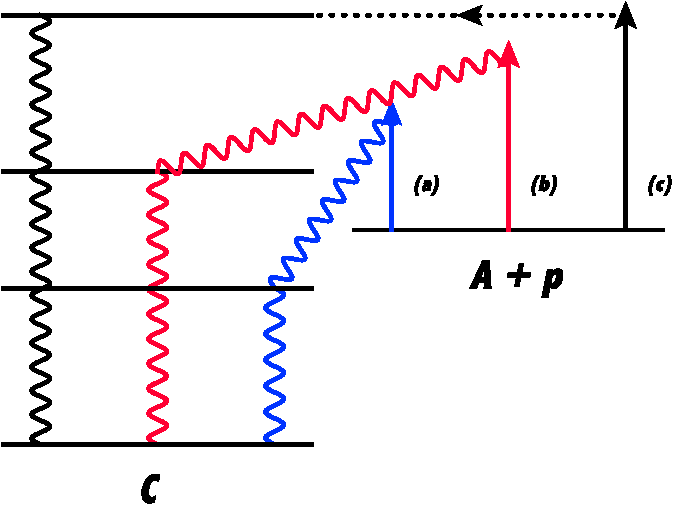
\includegraphics{radcap}
}
%\vspace{5cm}       % Give the correct figure height in cm
\caption{Energy level schematic showing various modes of radiative capture of a proton $p$ by a nucleus $A$ to form a product nucleus $C$. (a) represents direct capture into a bound state, (b) represents direct capture into an unbound (resonant) state, and (c) represents resonant capture into an unbound state.}
\label{fig:radcap}       % Give a unique label
\end{figure}


\subsection{Specifics of inverse kinematics}
\label{specifics}

In inverse kinematics, since the recoiling product nucleus is generally detected, it is important to consider the reaction kinematics in order to understand the final momentum spread and maximum laboratory angle of the recoil. Typical relative energies in the astrophysical regime, for processes occurring in novae and supernovae, can range up to the several hundred keV to MeV range. With typical inverse kinematics accelerated beam energies ranging up to around 2A MeV, the resulting beam velocities are usually below  $\approx0.05c$, and thus relativistic corrections are unnecessary. In the following discussion we will begin with relativistic expressions for kinematic variables for clarity, then reduce to or show alternative non-relativistic expressions where useful. We will also adopt the convention of {\em natural units} where the speed of light is equal to unity.

\subsubsection{Recoil and gamma ray energy and momentum}

In the inverse kinematics radiative capture reaction, the beam particle with laboratory energy $T'_{1}$ and mass $m_{1}$ is incident on the target particle of mass $m_{2}$, forming an excited compound nucleus with mass $m^{*}_{3}=m_{3}+E_{x}$. From energy conservation, it follows that the kinetic energy in the laboratory frame of the excited recoil is $T'^{*}_{3}=T'_{1}-E$ (the asterisk denoting the excited state), i.e. the laboratory kinetic energy of the beam minus the relative centre-of-mass energy of the beam+target. Thus, since subsequent emission of a gamma ray can only remove energy from the system, the kinetic energy of the recoiling nucleus is {\em always} smaller than the beam energy. If the ratio of beam to target mass is large, the recoil energy can be only a relatively small amount lower than the beam energy, a fact that becomes important for recoil separation techniques to be discussed later. 

The excited recoil nucleus then decays via emission of one or more gamma rays. In this example we will consider only one such decay to the ground state. Before the decay, by conservation of linear momentum, the excited nucleus has momentum  equal to that of the incident beam momentum: $(\vec{P}'_{3})^{*}=((E'_{3})^{*},0,0,(p'_{3})^{*})=\vec{P}'_{1}$, where we use the relativistic 4-momentum formalism, and define the z-axis to be the incident beam particle axis.  

The gamma ray is emitted (see fig. \ref{fig:kinematics}) in the C.M. system at an angle $\theta_{\gamma}$ w.r.t the z-axis (unprimed quantities are in the C.M. system). Since the recoil moves in a direction in the centre-of-mass system opposite to the gamma ray, we can combine the x- and y-coordinates and talk instead of the momentum components along the z-axis $(z)$ and perpendicular to the z-axis $(\perp)$. Thus the gamma ray will have momentum equal to $\vec{P}_{\gamma}=(E_\gamma, \vec{p}_{\gamma \left( \perp \right)}, p_{\gamma \left( z \right)})$,  while the recoil will have momentum  $\vec{P}_{3}=(E_{3},\vec{p}_{3 \left( \perp \right)},p_{3 \left( z \right)})$. To transform into the laboratory system we use the Lorentz transform equations\footnote{Note that the transformations are into the laboratory frame, which is moving in the direction of negative $z$ w.r.t. the beam direction from the point of view of an observer in the C.M. frame, hence the {\em inverse Lorentz transform} form of the equations are used.}:  

\begin{equation}
E'_{i}=\gamma(E_{i}+Vp_{i \left( z \right)})
\end{equation}
\begin{equation}
p'_{i \left( z \right)}=\gamma(p_{i \left( z \right)}+VE_{i})
\end{equation}
\begin{equation}
\vec{p}'_{i \left( \perp \right)}=\vec{p}_{i \left( \perp \right)}
\end{equation}
%
where $V=(p'_{3})^{*}/(E'_{3})^{*}$ is the velocity of the centre-of-mass system and $\gamma=(E'_{3})^{*}/m^{*}_{3}$ is the relativistic factor. 

These can be used to derive an exact expression for recoil kinetic energy:

\begin{equation}
\label{eqn:recoilenergy}
T'_{3}=\gamma(\sqrt{m_{3}^{2}+E_{\gamma}^{2}}-VE_{\gamma}\cos{\theta_{\gamma}})-m_{3}
\end{equation}
%
Evaluating this at $\theta_\gamma = \pi / 2$ and expanding the relativistic factor, $\gamma$, we get the {\em central kinetic energy} of the recoil:

\begin{equation}
T'_{3}=\frac{T'_{1}+Q+m_{2}}{m_{3}+E_{x}}\sqrt{m_{3}^{2}+E_{\gamma}^{2}}-m_{3}
\end{equation}

We can derive a similar expression for the laboratory gamma ray energy:

\begin{equation}
E'_{\gamma}=\gamma E_{\gamma}(1+V\cos{\theta_{\gamma}})
\end{equation}
%
and for the laboratory gamma ray angle:

\begin{equation}
\tan{\theta'_{\gamma}}=\gamma^{-1}\frac{\sin{\theta_{\gamma}}}{\cos{\theta_{\gamma}}+V}
\label{eqn:thetagamma}
\end{equation}
%
The latter two equations effectively show the Doppler effect on the gamma ray, resulting in a change in photon wavelength and direction in the laboratory frame. This effect also has the result of pushing flux in the backwards and forwards C.M. hemispheres forwards when transformed into the laboratory frame, resulting in a slight preference for flux in the forward laboratory frame. This has implications when considering to use gamma-ray hit-pattern information to deduce the reaction spatial origin in extended targets, as we shall see later on.  

\begin{figure}
\resizebox{1.0\columnwidth}{!}{
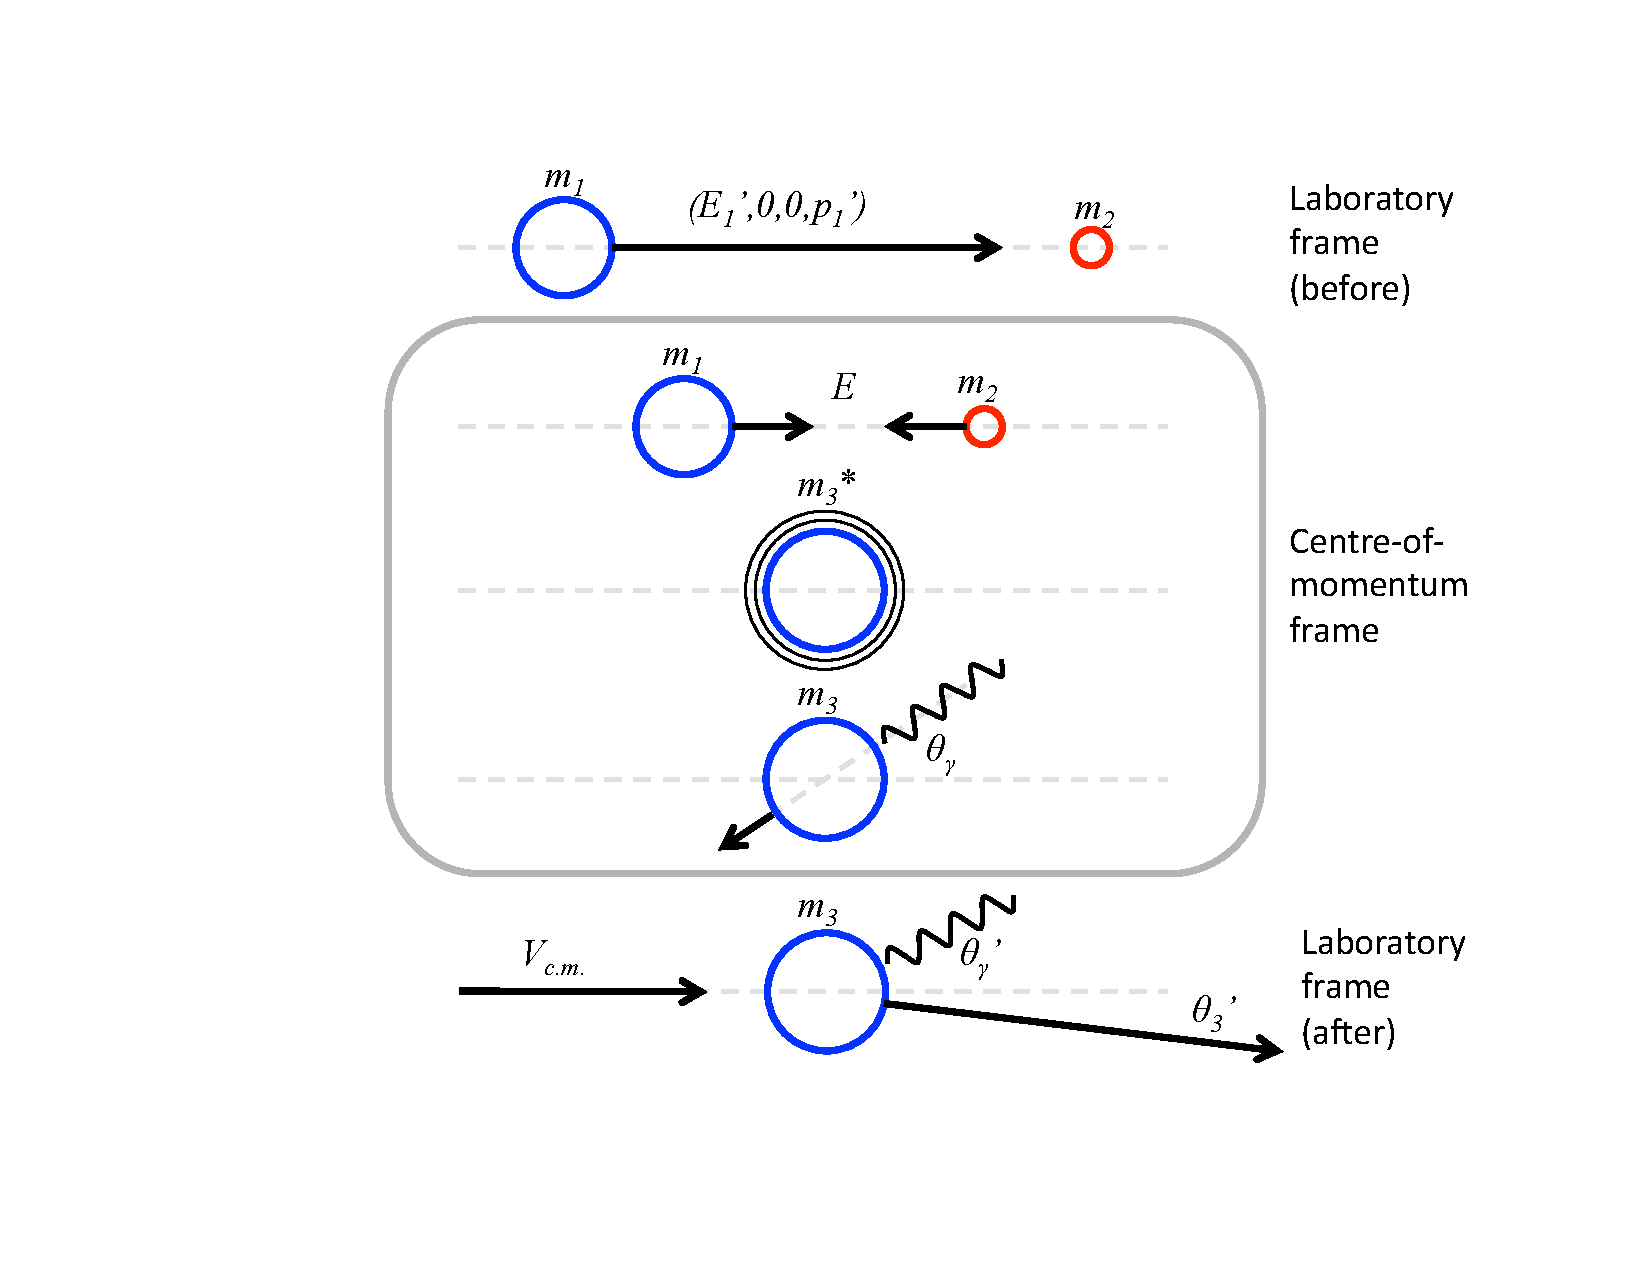
\includegraphics{kinematics}
}
%\vspace{5cm}       % Give the correct figure height in cm
\caption{Simplified schematic of kinematics of radiative capture reaction.}
\label{fig:kinematics}       % Give a unique label
\end{figure}

In addition, we can consider the momentum spread of the recoiling nucleus in order to quantify what range of momenta must be accepted in the recoil separator. Now, in the non-relativistic approximation, the maximum momentum spread of the recoil is given by the approximate relation:

\begin{equation}
\frac{\Delta p'_{3}}{p'_{3}}\simeq\frac{E_{\gamma,max}}{p'_{1}}\simeq\theta'_{3,max}
\end{equation} 

Thus a recoil separator designed to study the recoil products of such a reaction would need to accept momenta with $p'_{3}(1\pm\frac{\Delta p'_{3}}{p'_{3}})$. For typical beam velocities ranging from $(0.1-1.5)A\cdot$MeV at accelerator facilities interested in direct measurements, and for nuclei of interest in the range A=10-40, beam momenta can take on values anywhere between some hundred to over one thousand MeV/c. With reaction Q-values in the range anywhere from under an MeV to 10 MeV, in principle momentum spreads can take on values from fractions of one percent to several percent. Any recoil separator designed to measure such reactions must identify the range of reactions and meet the specifications for momentum acceptance therein.  

\subsubsection{Recoil angular distribution}

Returning to the Lorentz transformation expression, we can derive a similar expression to that of equation \ref{eqn:thetagamma} for the recoil particle:

\begin{equation}
\tan{\theta'_{3}} = \frac{\sin{\theta_{3}}}{\gamma(V/v_{3}+\cos{\theta_{3}})}
\end{equation}
%
Here, $v_{3}$ is the recoil velocity in the centre-of-mass frame given to the product nucleus due to the emission of the $\gamma$ ray, and $\theta_{3}$ is the angle of the recoiling nucleus in the centre-of-mass frame with respect to the incident beam particle direction. The maximum recoil angle that can possibly occur is when the energy of the emitted $\gamma$-ray is maximized ($E_{\gamma}=Q+E$), where $E$ is the relative energy of target and projectile in the centre-of-mass\footnote{ $E=\sqrt{2m_{2}(T'_{1}+m_{1})+m_{1}^{2}+m_{2}^{2}}-m_{1}-m_{2}$, and in the non-relativistic approximation $E=\frac{m_{2}}{m_{1}+m_{2}}T'_{1}$ }, and the emission occurs perpendicular to the incident beam direction ($\theta_{3}=\pi/2$) so that:

\begin{equation}
\tan{\theta'_{3,max}}=\frac{v_{3}}{\gamma V}
\end{equation} 
%
It can be shown that in the non-relativistic limit this can be approximated by:

\begin{equation} \label{eq:6}
\tan{\theta'_{3,max}}\simeq\frac{Q+E}{\sqrt{2\frac{m_{1}}{m_{2}}(m_{1}+m_{2})E}}
\end{equation}
%In the following discussion we assume a projectile of mass $m_{1}$, momentum $p_{1}$ and kinetic energy $T_{1}=p_{1}^{2}/2m_{1}$ is incident on a stationary target particle of mass $m_{2}$.   
%The relative energy in the centre-of-mass system is given by:\footnote{The fully relativistic expressions are: $T_{1}=\sqrt{p_{1}^{2}+m_{1}^{2}}-m_{1}$ and $E_\mathrm{c.m.}=\sqrt{2m_{2}(T_{1}+m_{1})+m_{1}^{2}+m_{2}^{2}}-m_{1}-m_{2}$, with all energies in units of MeV and all masses in units of MeV/$c^{2}$.  }
%
%\begin{equation}
%E_\mathrm{c.m.}=\frac{m_{2}}{m_{1}+m_{2}}T_{1}
%\end{equation} 
It is interesting to note that this relation has a minimum ($\frac{d\theta'_{3,max}}{dE}=0$) when $E=Q$. Figure \ref{fig:coneangles} shows the maximum recoil half-angle in the laboratory frame versus centre-of-mass energy, for a variety of astrophysically interesting radiative capture reactions. As shown by equation \ref{eq:6}, the position of the minimum and therefore the local behaviour of the functions is determined by the reaction $Q$-value. For example the $^{7}$Be($p,\gamma$)$^{8}$B reaction which has a $Q$-value of only $0.138 \unit{MeV}$, generally has the maximum recoil half-angle increasing with increasing centre-of-mass energy above this value. On the other hand the $^{23}$Na($p$,$\gamma$)$^{24}$Mg reaction, with $Q=11.693 \unit{MeV}$, generally has its maximum recoil half-angle decrease with increasing beam energy over the astrophysically relevant energy range. This has implications for the geometric acceptance of recoil separators built to study such reactions. 

Of course the above discussion only tells us what the maximum possible recoil angle is in the event that the entire centre-of-mass energy is converted by emission of a single gamma ray to the recoil ground state, and says nothing of the distribution of the recoil directions. In the event of a multiple-gamma cascade, each decay will proceed in some direction in the centre-of-mass system resulting in a recoil laboratory polar angle less than the maximum possible in a single decay. In rare occasions the momentum vectors of these decays can line up to reach the equivalent of a single gamma ray, but more usually they will be unaligned, with the probability of alignment dropping rapidly with the number of gamma rays in the cascade. The result is that the most probable recoil angle, or the mean recoil angle, will be less than the maximum angle. In addition, the in-target angular straggling and divergence of the incoming beam will in general broaden the resulting distribution.
To illustrate this, Figure \ref{fig:26altheta} shows a kinematic simulation for resulting recoil polar angles for the $^{26}$Al($p,\gamma$)$^{27}$Si reaction on the $E_{c.m.}$=188 keV resonance, originating at the centre of an extended gas target, using realistic values of incident beam energy spread, transverse emittance and straggling. Shown are two different cases, one where the gamma decay from the resonating $^{27}$Si state goes 100$\%$ to its ground state, the other where the decays proceed through a series of cascades, with no gamma decay direct to the ground state. The maximum recoil polar angle allowed by kinematics in such a case is 15.6 mrad, however the incident beam properties mentioned above conspire to increase this maximum slightly. 
One can immediately see from the figure that for a finite angular acceptance recoil separator or detector cutting into the angular distribution, the effect on detection efficiency is much more severe in the case of 100\% ground state decay than in the case of the cascade. It is thus important to know the branching ratios of such decays in advance if the angular acceptance of the recoil separator/detector is close to the maximum recoil angle. If branching ratios are completely unknown, simulations can determine efficiencies, and combined with detected gamma ray information, can lead to a determination of branching ratios.    

\begin{figure}
\resizebox{\columnwidth}{!}{
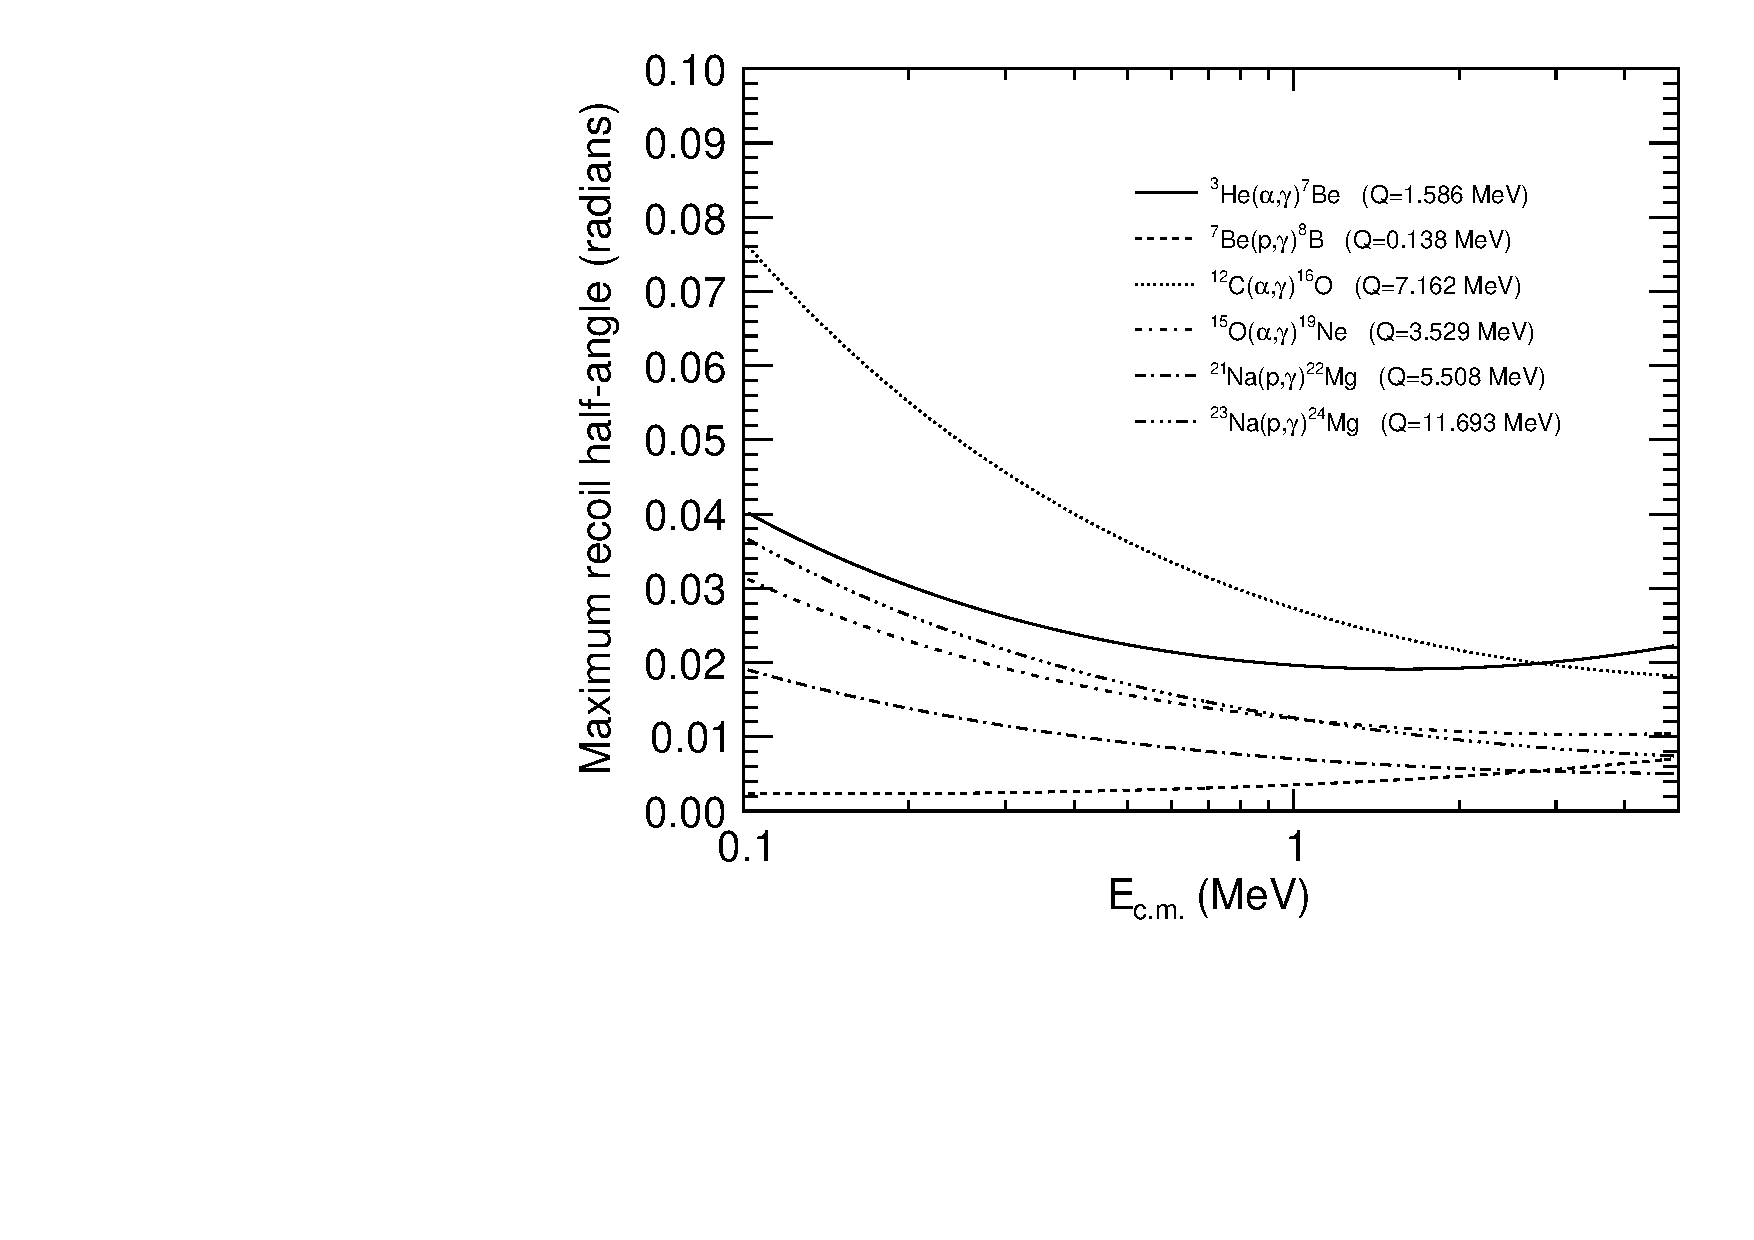
\includegraphics{coneangles}
}
%\vspace{5cm}       % Give the correct figure height in cm
\caption{Maximum recoil half-angle as a function of centre-of-mass energy, for a variety of interesting radiative capture reactions.}
\label{fig:coneangles}       % Give a unique label
\end{figure}

\begin{figure}
\resizebox{\columnwidth}{!}{
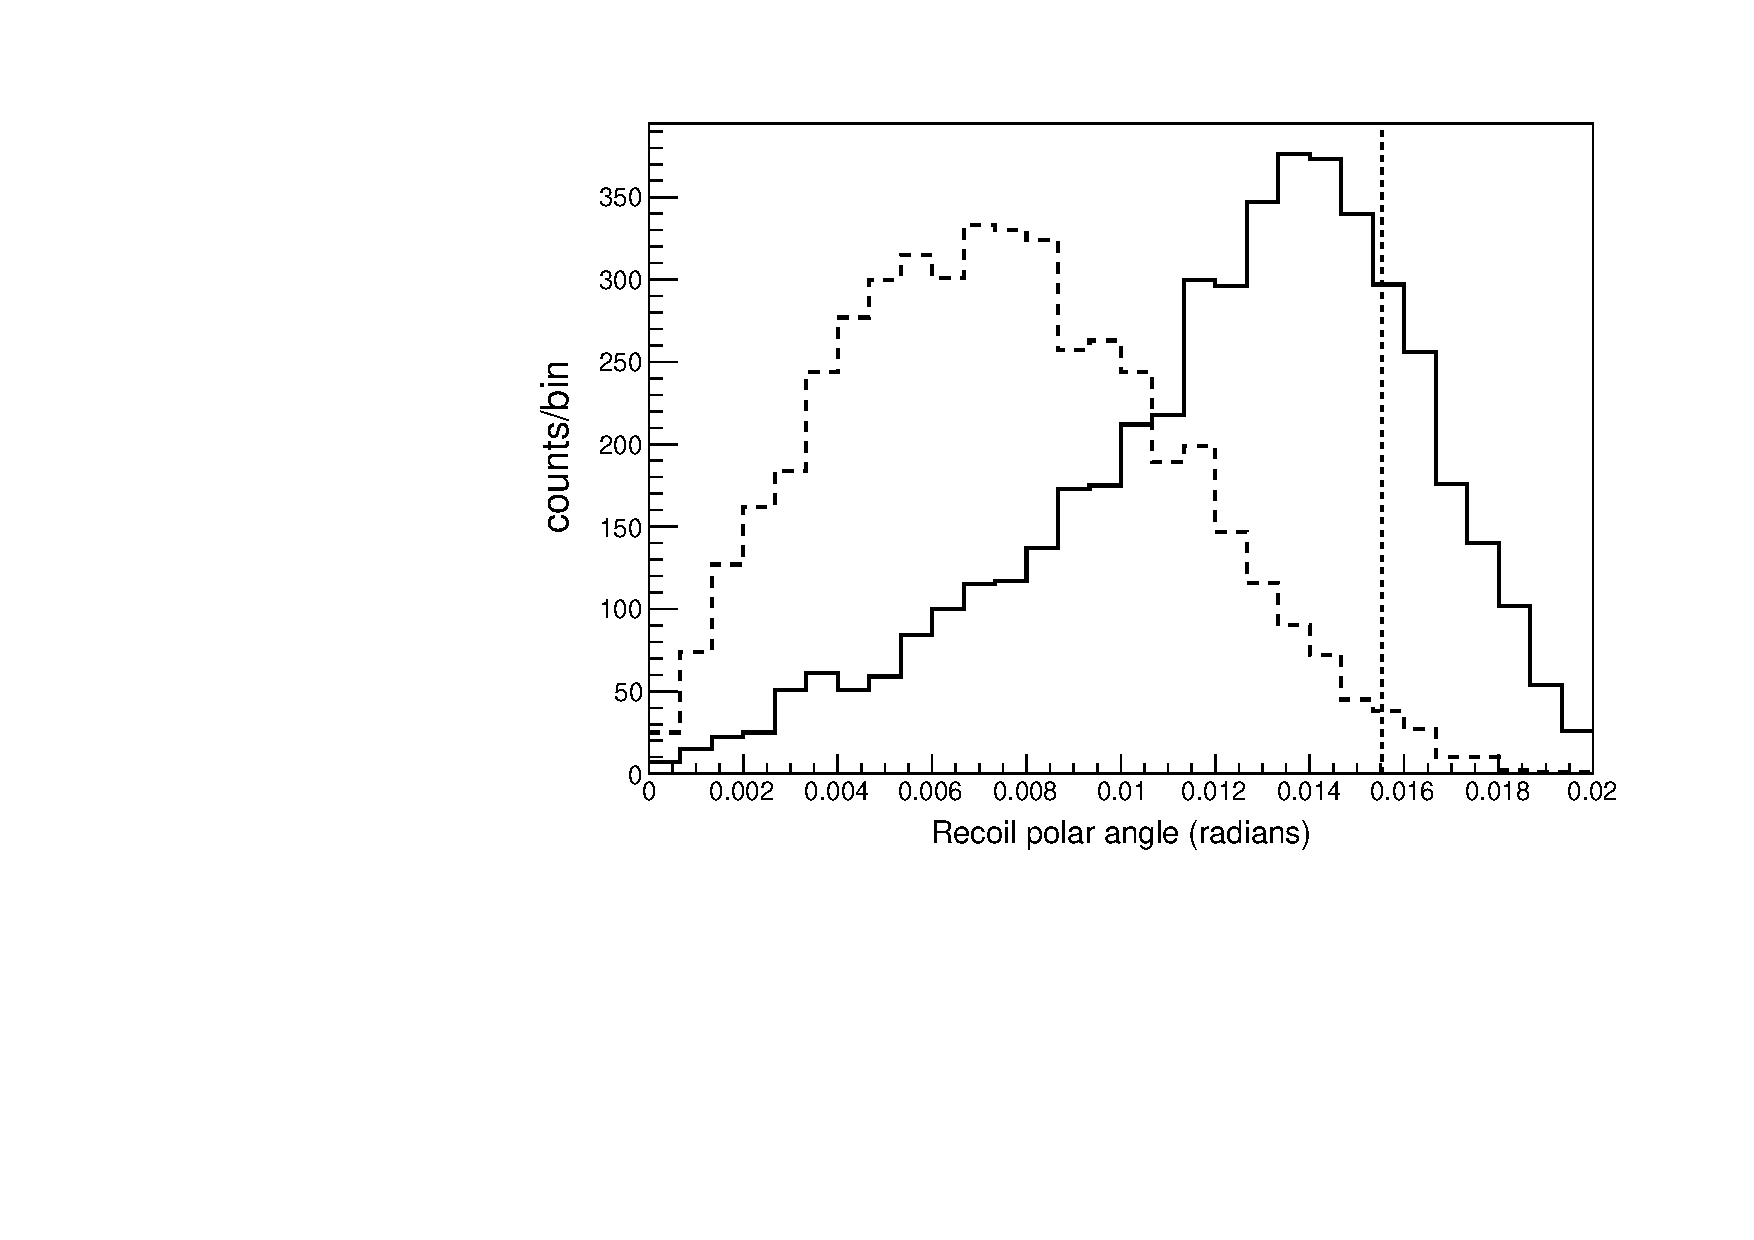
\includegraphics{26altheta}
}
\caption{Hypothetical inverse kinematics distribution of recoil angles emerging from the $^{26}$Al($p,\gamma$)$^{27}$Si reaction at $E_{c.m.}$=188 keV in an extended gas target, using realistic values of beam emittance, energy spread, and straggling (isotropic gamma ray angular distribution in the C.M. system). The solid histogram shows the case where 100\% of decays are to the ground state; the dashed histogram shows the case for a series of cascade gamma rays. The dotted line shows the maximum possible recoil angle in the case of perfectly aligned incident beam particles. }
\label{fig:26altheta}       % Give a unique label
\end{figure}

\subsubsection{$\gamma$-ray angular distribution and effect on recoil angle and energy} 

The angular distribution of the gamma rays in the centre-of-mass system also plays a role in determining the recoil angular (and energy) distribution. Since we are considering the effect on the recoil angular distribution, we are talking here about the cumulative effect of several gamma rays in a cascade. In principle, this depends in a complicated fashion on the spins of the nuclear levels and the multipole mixing ratios of the gamma transitions. For simplicity, we consider the case where the initial transition is to the ground state or to a very low-lying excited state, so that subsequent transitions (if any) have negligible impact on the momentum of the heavy recoil particle. In addition, most of the low energy radiative capture reactions interesting for astrophysics will proceed via low orbital angular momentum transfer into a resonant state. For direct capture the situation can be complicated and is not considered here, but for individual narrow resonances, states of definite $J^{\pi}$ are populated.

For s-wave proton capture, the distribution of initial $\gamma$ decays will be isotropic in the centre-of-mass frame. This is because it is clear that when $\ell=0$ the compound nuclei are formed with no preferred axis, as the unpolarized initial beam and target spins combine randomly. Thus although each {\em individual} $\gamma$ decay (which can in principle be an admixture of multipolarities) will certainly have some non-uniform angular distribution with respect to the preceding newly-formed spin axis of the excited nucleus, the distribution of directions of all decays will be uniform over a sphere in the centre-of-momentum system. In the case of initial s-wave capture into a series of cascade transitions, one can expect subsequent decays to be randomly oriented with respect to the beam axis as well even though the angle between two successive decays from the same nucleus will be correlated. The magnitude of the vector sum of the decays will differ according to the correlations however. Thus for the purposes of calculating the effect on the final distribution of recoil angles, s-wave captures can to a good approximation be thought of as isotropic decays in the C.M. frame for a single decay to the grounds state, and,  if the angular correlations between decays are small in magnitude, also for cascade transitions.  

In the case of p-wave proton capture, anisotropy is possible when the spin, $J$, of the resonant state is greater than the sum of the intrinsic spins of the projectile and target. The orbital angular momentum $\ell$ has a component only in the $m=0$ state, with the result that the magnetic substates of the resonant level having projection $M=\pm J$ cannot be populated. The system is not spherically symmetric and the gamma rays show some anisotropy.

The special case of spin-zero projectile and target nuclei, i.e. $\alpha$-capture on a spin-zero nucleus, can result in large anisotropies in the initial $\gamma$-ray angular distribution with respect to the beam axis and thus the recoil angular distribution. This is because the channel spin, $s=0$ and thus the compound nucleus is formed purely by coupling to the orbital angular momentum quantum number, $\ell$. When this is non-zero, it causes the system to align with the momentum vector of the beam nucleus, i.e. the beam axis. Subsequent multipole decay angular distributions will therefore be reflected in the recoil angular distribution with respect to the beam axis. Strong dipole and quadrupole distributions can be found for example in the recoil energy spectra from resonances in the \nuc{12}{C}\reac{\alpha}{\gamma}\nuc{16}{O} reaction \cite{mat06}, with the relationship between recoil energy and $\gamma$-ray angle being given by eqn. \ref{eqn:recoilenergy}. 

%\subsection{Experimental requirements theory of separators, and figures of merit}

%\small
%\begin{itemize}
%\item Do we want to do an opening angle figure ( opening angle as a function of mass with different lines for different max Eg = Q+ Ecm emitted)?
%\item Recoil separator capable of accepting the recoil angle of the specific reaction targeted
%\item combination of recoil separator and focal plane detector capable of separating beam and reaction recoils
%\item additional use of g-detector array
%\item what are typical: g-ray energies (multiplicity); momentum distribution; opening angles; target thickness; geometry; stopping; straggling; charge state distributions
%\item Is there a time structure of the beam; other beam properties; what are the minimum beam properties needed?
%\end{itemize}
%\normalsize
      % Introduction

%%%%%%%%%%%%%%%%%%%%%%%%%%%%%%%%%%%%%%%%%%%%%%%%%%%%%%%%%%%%%%%%%%%%%%%%%%%
%%%%%%%%%%%%%%%%%%%%%%%%%%%%%%%%%%%%%%%%%%%%%%%%%%%%%%%%%%%%%%%%%%%%%%%%%%%
\section{Design Principles of Recoil Separators}
% Experimental requirements, theory of separators, figures of merit
\label{design}

In this section we will present the equations for the motion of charged particles in magnetic and electric fields before discussing the types and design of ion-optical elements required in different designs of recoil separators, as well as exploring some of the rigidity and performance regimes for astrophysically important radiative capture reactions. In addition we discuss the various types of gas targets that can be used with a recoil separator.

%%%%%%%%%%%%%%%%%%%%%%%%%%%%%%%%%%%%%%%%%%%%%%%%%%%%%%%%%%%%%%%%%%%%%%%%%%%
\subsection{Ion Optical Elements}
\label{ion}

For a recoil separator to function, it in principle has to induce a spacial separation between unreacted beam and recoil particles of different mass but similar momentum. In addition, it has to accept recoils with divergent angles with respect to the beam axis. In almost all cases discussed in this paper polarized beams are not used, therefore recoils are uniformly distributed in azimuthal angle, $\phi$. 
Thus in order for recoils to be separated, they must be brought to a focus in a mass-dispersed plane at some point. Due to the typical rigidities experienced in inverse kinematics at astrophysically-relevant energies, magnetic elements are required to provide the focusing. Electrostatic elements or combined electrostatic and magnetic elements can be used in addition to these to provide mass dispersion or beam rejection.  

The motion of a charged particle (with charge $q$) in external electromagnetic fields $\vec{E}$ and $\vec{B}$  is governed (non-relativistically) by the Lorentz force equation:

\begin{equation}
\vec{F}=q(\vec{E}+\vec{v}\times\vec{B})
\end{equation}   

where $\vec{v}$ is the instantaneous particle velocity. 



%%%%%
\subsubsection{Magnetic elements -- focussing and momentum/charge dispersion}\label{magel}

%\small
%\begin{itemize}
%\item What are the necessary equations to present?
%\item path of a charged particle in a magnetic field
%\item image/object relationship
%\item typical field strengths
%\item double focussing, sextupole correction
%\item its function as a momentum filter in our application means that we use it as a charge state filter because beam and reaction recoil have very similar central momentum
%\item give equation for position of charge states blocked by slits
%\end{itemize}
%\normalsize

Magnetic quadrupoles are required in order to produce foci for the transported ions in the separator. This is usually achieved via doublets or triplets, providing net focussing in both the horizontal and vertical planes. While doublets are suitable for the bulk of the focussing\footnote{Note that an antisymmetric doublet, one whose field gradients and effective lengths are equal, cannot provide a true stigmatic focus, instead transforming a circular source image into an ellipse. With a general doublet however stigmatic operation is possible \cite{reg67}.}, triplets may be required prior to a focus with more stringent requirements. This is due to the fact that in doublets changes in field strength in one focussing plane might introduce undesirable changes in the other plane. Triplets offer an extra degree of freedom to work with in obtaining the focal properties of interest.  

Quadrupoles have focal lengths that are rigidity- and field-gradient-dependent, and thus which must have the applied field scaled according to the ion charge, mass and energy.  With typical effective lengths of quadrupole magnets usually on the order of 0.2-0.5 metres for the momenta under consideration here, the strengths required for effective focussing will depend on the field gradient required and thus the quadrupole bore, but for most recoil separator applications, field strengths are on the order of 0.1 Tesla at the pole tip. Due to the difficulty of achieving perfect focussing properties using simple quadrupole doublets and triplets, higher order multipole magnets are used to make corrections for aberrations induced by the quadrupoles. Primarily, separate sextupole magnets can be combined with the doublets and triplets. These correct for the typical spherical and `coma'-type aberrations. In addition, quadrupole magnets can be constructed with pole-tip shaping that induces a sextupole or higher-order component.  

Beam-target and recoil-target interactions will result in a distribution of ion charge-states being propagated through the separator. In order to bring the ions to a unique mass-dispersed focus there must be some form of momentum-charge filter. The least complex way to do this would be the use of a magnetic dipole field in combination with quadrupole focussing. A magnetic dipole placed after a stigmatic doublet would provide dispersion in momentum-charge space. Simplistically (neglecting fringe fields), from the Lorentz equation and the equation of circular motion through the dipole field it can be shown that rays of rigidity $B\rho$ moving along the ion-optical axis will, to first-order satisfy the relation:
\begin{equation}
B\rho=\frac{p}{q}
\end{equation}

Thus it can be seen that since recoil ions will typically vary only within $\pm2\%$ or so of the beam momentum value, such a device cannot be used as a mass separator, with bending angles being very close to each other for a given charge state. However since neighbouring integer charge states are usually different by a large fraction of the charge state value, bending angle differences are larger. This means spacial separation of neighbouring charge states can be significant in the focal plane, and slits can be used to reject the unwanted components. One can say to a good approximation that $\Delta \rho / \rho \approx \Delta q / q$. In addition, a low energy tail in the beam/recoils, perhaps induced by electrostatic elements in the accelerator or even small angle scattering within the separator target region, can be rejected after this device. In practice, magnetic dipoles will have shaped pole edges that mitigate field-gradient issues that would otherwise result in focussing problems.

%%%%%
\subsubsection{Electrostatic elements}

%\small
%\begin{itemize}
%\item path of a charged particle in an electrostatic field
%\item typical necessary field strength/curvature for our application
%\item focussing issues
%\item acts as an energy filter
%\item where does the not transmitted beam/charge states end up (split electrode approach, gridded possibility?)
%\end{itemize}
%\normalsize

A cathode and anode in the form of segments of concentric cylinders can produce a radial electric field which has constant magnitude $\mathcal{E}$  at a constant distance from the axis of the cylinders.   Ions having a suitable electric rigidity can travel at a constant radius through the device. Such an electrostatic dipole will deflect reaction products and beam ions through different angles due to their different velocities, resulting in differing $x$ positions in the focal plane given by $x-x_0\approx\frac{p(v-v_0)}{q\mathcal{E}}$. Such separation, as a fraction of the bending radius, will be on the order of the fractional beam-recoil mass difference, which will always be larger than the spread in recoil momenta. Thus at such a mass-dispersed focus, slits can be placed to provide beam rejection while allowing the recoil ions to pass through.   However, a low-energy tail of the beam, in a lower charge state and having the same electric rigidity as the reaction product, will not be separated. This short-coming can be remedied by combining a magnetic dipole and electrostatic dipole in such a way that a subsequent angular focus is also a focus in ion energy (achromatic) but is dispersed according to ion mass.  

The required electrostatic fields are of order megavolts per metre.  Extensive measures, such as polishing the electrodes to a mirror finish, are required to prevent voltage breakdowns.   Because an electrostatic dipole must deflect desired particles through a permanently-fixed angle,  an experiment  cannot be performed unless the requisite   electrode voltages can be achieved. A CW multiplier stack can be used to achieve the high voltages on the electrodes. The usual design of such a device consists of a steel vacuum tank containing the electrodes, and two cylindrical stack regions containing the multiplier and filled to overpressure with an inert insulating gas such as SF$_{6}$, though devices with external high-voltage supplies could be considered depending on the separator layout geometry. The devices are prone to electrical breakdown in the region between the electrodes due to impurities on the electrode surface or other non-uniformities like `whiskers' of electrode metal that can form. In each case breakdown results in the generation of x-rays with a spectrum dependent on the applied voltage. Therefore a significant amount of shielding is required on the device to protect users from radiation fields during any conditioning phase of the electrodes. 

Conditioning of these devices consists of slowly stepping up the voltage allowing the generation of sparks that will produce an allowable flux of x-rays, stepping back down in voltage when the flux climbs above a predetermined threshold. These sparks will burn off the impurities that cause them, allowing an overall voltage increase. Once operational voltage is achieved the ambient x-ray flux should be negligible and in principle the electrodes hold their conditioning under vacuum indefinitely at high voltage, self-regulating any impurities. Long periods at lower voltage can cause the conditioning to be lost, as can a drastic change in vacuum properties. In the case of `whisker' impurities, inert moderately heavy gas such as argon can be introduced to the system during conditioning, the idea being that ions are made during sparks that can provide enough energy to etch away the whisker. As will be seen in later sections, such devices have successfully achieved field gradients of up to 4.6 MV/m.  

%%%%%
\subsubsection{Combined crossed field (Wien) filter elements}

%\small
%\begin{itemize}
%\item what conditions have to be met to transmit the recoils (E,B field selection, condition)
%\item what is the equation which tells us where the not transmitted beam and other charge states end up
%\item typical fields and dimensions for our application
%\end{itemize}
%\normalsize

In a Wien filter parallel flat electrodes between the poles of a magnet provide crossed electric and magnetic fields, $\mathcal{E}$ and $B$.      There is a certain ratio $\mathcal{E}/B$ which results in ions of velocity $v$  undergoing no deflection as they pass through the Wien filter, regardless of their momentum $p$ or charge $q$.    Accordingly, a Wien filter can be tuned to pass the desired reaction product straight through while deflecting beam ions.  Like the electrostatic dipole, it may pass beam particles in  a low-energy tail; unlike the electrostatic dipole, it  also allows   neutral particles to pass through.

Because it is  the ratio $\mathcal{E}/B$ which selects the velocity, a Wien filter may operate with reduced\ field strengths (and reduced mass resolving power)  in order to accommodate reaction products of high rigidity, or if there is a problem reaching the designed maximum electric field.    On the other hand, a Wien filter poses greater design problems, requiring careful shaping of both the electrodes and the magnet poles in order to achieve the desired field uniformities and to match fringe fields. 

In general a Wien filter suffers from the same high voltage conditioning constraints as electrostatic dipole devices,. In addition, because of the geometry of a Wien filter external high voltage supplies such as used in some muon spin rotator systems (e.g. M20 facility, TRIUMF \cite{bev85}) can be used. 

%%%%%%%%%%%%%%%%%%%%%%%%%%%%%%%%%%%%%%%%%%%%%%%%%%%%%%%%%%%%%%%%%%%%%%%%%%%
\subsection{Performance}
\label{performance}

%%%%%
\subsubsection{Beam suppression}
Reaction yield and detector performance together define the requirements for beam suppression by the separator.    The most challenging reactions  may well call for suppression by 10 to 12 orders of magnitude.    Separator designs for fusion-evaporation reactions, with higher yields and larger beam-product mass differences, may not be the best models  for radiative capture experiments.   
    
 One class of potential background is the tail of a  distribution generated by many small interactions, such as multiple scattering or energy straggling in the target.    Typically, these distributions have a Gaussian shape near their maximum but after only a few  ``standard deviations" the distributions become dominated by single large-deviation interactions, such as nuclear scattering in the target.    More complicated to assess are single scatterings from residual gas somewhere within the separator.   Nevertheless, it may be possible to investigate by computer simulation whether  a proposed separator design is able to suppress such events.
 
  ``Black Swan" events pose the most difficult problem for the separator designer.   By definition extremely rare and hard to foresee,  they are not  amenable to realistic simulation by computer.   Typically, they may involve sequential scatterings from  solid surfaces inside the separator.   The ranges of beam ions in solids being on order 1--10~$\mu$m, the surface material and roughness at the micrometer scale play a big role: oblique incidence on a smooth surface should be avoided and if possible such surfaces should be masked.   The separator designer must look to defense in depth, with more beam suppression features than the minimum required for events of the first  class.

%%%%%
  \subsubsection{Figure of merit}
  Some specifications, taken in combination, impose minimum requirements on the strength and extent of electric and magnetic fields.   These are the mass resolving power ($P_\mathrm{m}$), the angular acceptance ($\Delta a$) and the maximum particle rigidity 
  ($\mathcal{R}_\mathrm{M}=p/q$ or $\mathcal{R}_\mathrm{E}=pv/q$).    
  Consider a source of ions (reactions in the target), a dispersive device  (radius of curvature $\rho$) and an image (focus) point.   The  trajectories of the ions having the extremes in initial angles will delimit an area ($A$)  in the bend-plane of the dispersive device.     To first order the resolving power is given by the linear magnification ($M$) of the image, the mass dispersion ($D$) and the transverse source size ($\Delta x$): 
  $P_\mathrm{m} = D/(M \cdot \Delta x) $. 
  It has long been known (see, for example, \cite{Wo71}) that source emittance and the resolving power can be related to properties of the dispersive device by
  \[ P_\mathrm{m}\  \Delta a\  \Delta x = A/\rho \]
  Recalling that 
  $\mathcal{R}_\mathrm{M}=\rho \ B$ and $\mathcal{R}_\mathrm{E}=\rho \ \mathcal{E}$,  we obtain  figures of merit 
  \[ P_\mathrm{m}\  \Delta a\  \Delta x \ \mathcal{R}_\mathrm{M} = A \cdot B \]
   \[P_\mathrm{m}\  \Delta a\  \Delta x \ \mathcal{R}_\mathrm{E} = A \cdot \mathcal{E} \]
   That is, to achieve a certain figure of merit it is necessary to have a certain minimum product of field strength and area.  For an electrostatic device it may be convenient to use the length of electrodes and the gap between them as a proxy for the area $A$.  Then, the figure of merit becomes $L\cdot\Delta V$, where $L$ is the length of the electrodes and $\Delta V$ is the voltage difference between them.
   
%%%%%
\subsubsection{Charge changing cross sections}
One factor to consider in separator design is the vacuum requirements over the separator length. Residual gas in the separator can result in the ions of selected charge state acquiring or losing electrons through atomic collisions. Such single charge-changing events will not make it to the end of the separator due to the rigidity change, and this effect results in an overall loss of detected flux of recoils at the end of the separator.  In addition, as previously mentioned, beam ions that would otherwise be rejected by electromagnetic devices can undergo charge-changing collisions, removing efficacy of the separator beam suppression.

As an example of the magnitude of such effects, Schlachter {\em et al.} \cite{sch83} provide an empirical scaling law for electron capture on fast highly-charged ions in gas. Using their relations, it can be seen that for light ions $(A<40)$ in the energy regime $(100-1500)A$ MeV, typical electron capture probabilities range from 5\% at the low energy, high mass end, to tenths of a percent at the high energy end when the vacuum pressure is in the range $1\times10^{-6}$ torr over a 10 m length of the separator. Thus, for longer separators, maintaining good high vacuum over as much of the length as possible is recommended, and where possible and where cost permits, try to achieve vacuum in the $10^{-7}-10^{-8}$ torr range over significant portions of length, for example in electrostatic devices. However, for the majority of cases in the astrophysical mass and energy regime, and the typical rigidities selected the charge-changing effect is small enough to be absorbed by other overarching uncertainties in for example, beam normalization and detection efficiency. 



%%%%%
\subsubsection{Additional factors} 
  Windowless targets either extended gas cell or gas jet, can impose major constraints on separator design.  Tubes between differential pumping stages may limit the convergence of incoming beam and consequently limit how small the beamspot  can be made at the target.  Pumping stages may set a minimum distance from target to the first focusing element.

Detectors of the heavy reaction product may have a maximum counting rate for optimum resolution, requiring a matching minimum beam suppression factor for the separator.   The detector may be limited in size, requiring a correspondingly small envelope of trajectories.    Good energy resolution or particle identification in a detector may permit a higher rate of beam leakage through the separator.

 The space   for the separator may be limited or the wrong shape if the experimental area was designed for the needs of earlier experiments.   Dipoles, quadrupoles  or Wien filters from elsewhere  may be available for use.  Finally,  funds for the project may be limited.   

%%%%%%%%%%%%%%%%%%%%%%%%%%%%%%%%%%%%%%%%%%%%%%%%%%%%%%%%%%%%%%%%%%%%%%%%%%%
\subsection{Gas targets}
\label{gas}

%%%%%
\subsubsection{Windowless targets and differential pumping}


For our purpose of measuring proton or alpha radiative capture in inverse kinematics, a hydrogen or helium gas target is required which has sufficient density  to contain energetically the targeted resonance width or a sufficient direct capture interval to provide a measurable yield. Additionally, the uncertainty of a resonance position --- from transfer reaction measurements and nuclear mass information --- has to be taken into account. As the resonant yield is inverse proportional to the target stopping power it is also beneficial to avoid inactive nuclei in its composition, {\it e.g.} a pure hydrogen target provides a factor 3--4 higher yield than a CH$_2$ foil target.  A gas target is also virtually indestructible and stable in its composition while in plastic foil targets the carbon to hydrogen ratio is known to change even under modest heavy ion beam flux on the order of $10^7 \unit{s^{-1}}$.


In order to achieve a target thickness of 10 keV (in the centre-of-mass system) with the light to medium mass ion beams in question at astrophysically relevant energies, a target number density of approximately $5\times10^{18} \unit{nuclei~cm^{-2}}$ of hydrogen is required. To provide unimpeded beam and recoil transmission, the gas cannot be confined by foil windows, leaving as the only possible approach the use of a windowless, differentially pumped gas target. The gas pressure necessary to achieve the required target number density is given by the formula \cite{rolf88} 
\begin{equation}
n_A = 9.66\times10^{18} L \nu \frac{P}{T}~\mathrm{[cm^{-2}]}
\end{equation}
with $L$ the target length in cm, $\nu$ the number of atoms per molecule, $P$ the pressure in Torr, and $T$ the temperature in K.\\
It should be noted that the target length needs to be kept small ($<$ 10--15 cm) in order not to significantly increase the acceptance requirements for the recoil separator. The windowless approach means that a target pressure of a few torr needs to be maintained in the gas cell, but a reduction to the order of $10^{-6} \unit{torr}$ achieved over several gas flow limiting apertures and pumping stages is necessary to allow connection to the accelerator and separator. On the accelerator side the dimensions of these apertures are defined typically by the beam dimensions, while on the separator side the reaction recoil cone needs to be accommodated. Therefore, it is preferable to compress the length of the differential pumping stages as much as possible to allow for smaller aperture sizes. A typical pumping scheme is depicted in Fig. \ref{fig:dragon_pumping}.
\begin{figure}
\resizebox{0.9\columnwidth}{!}{
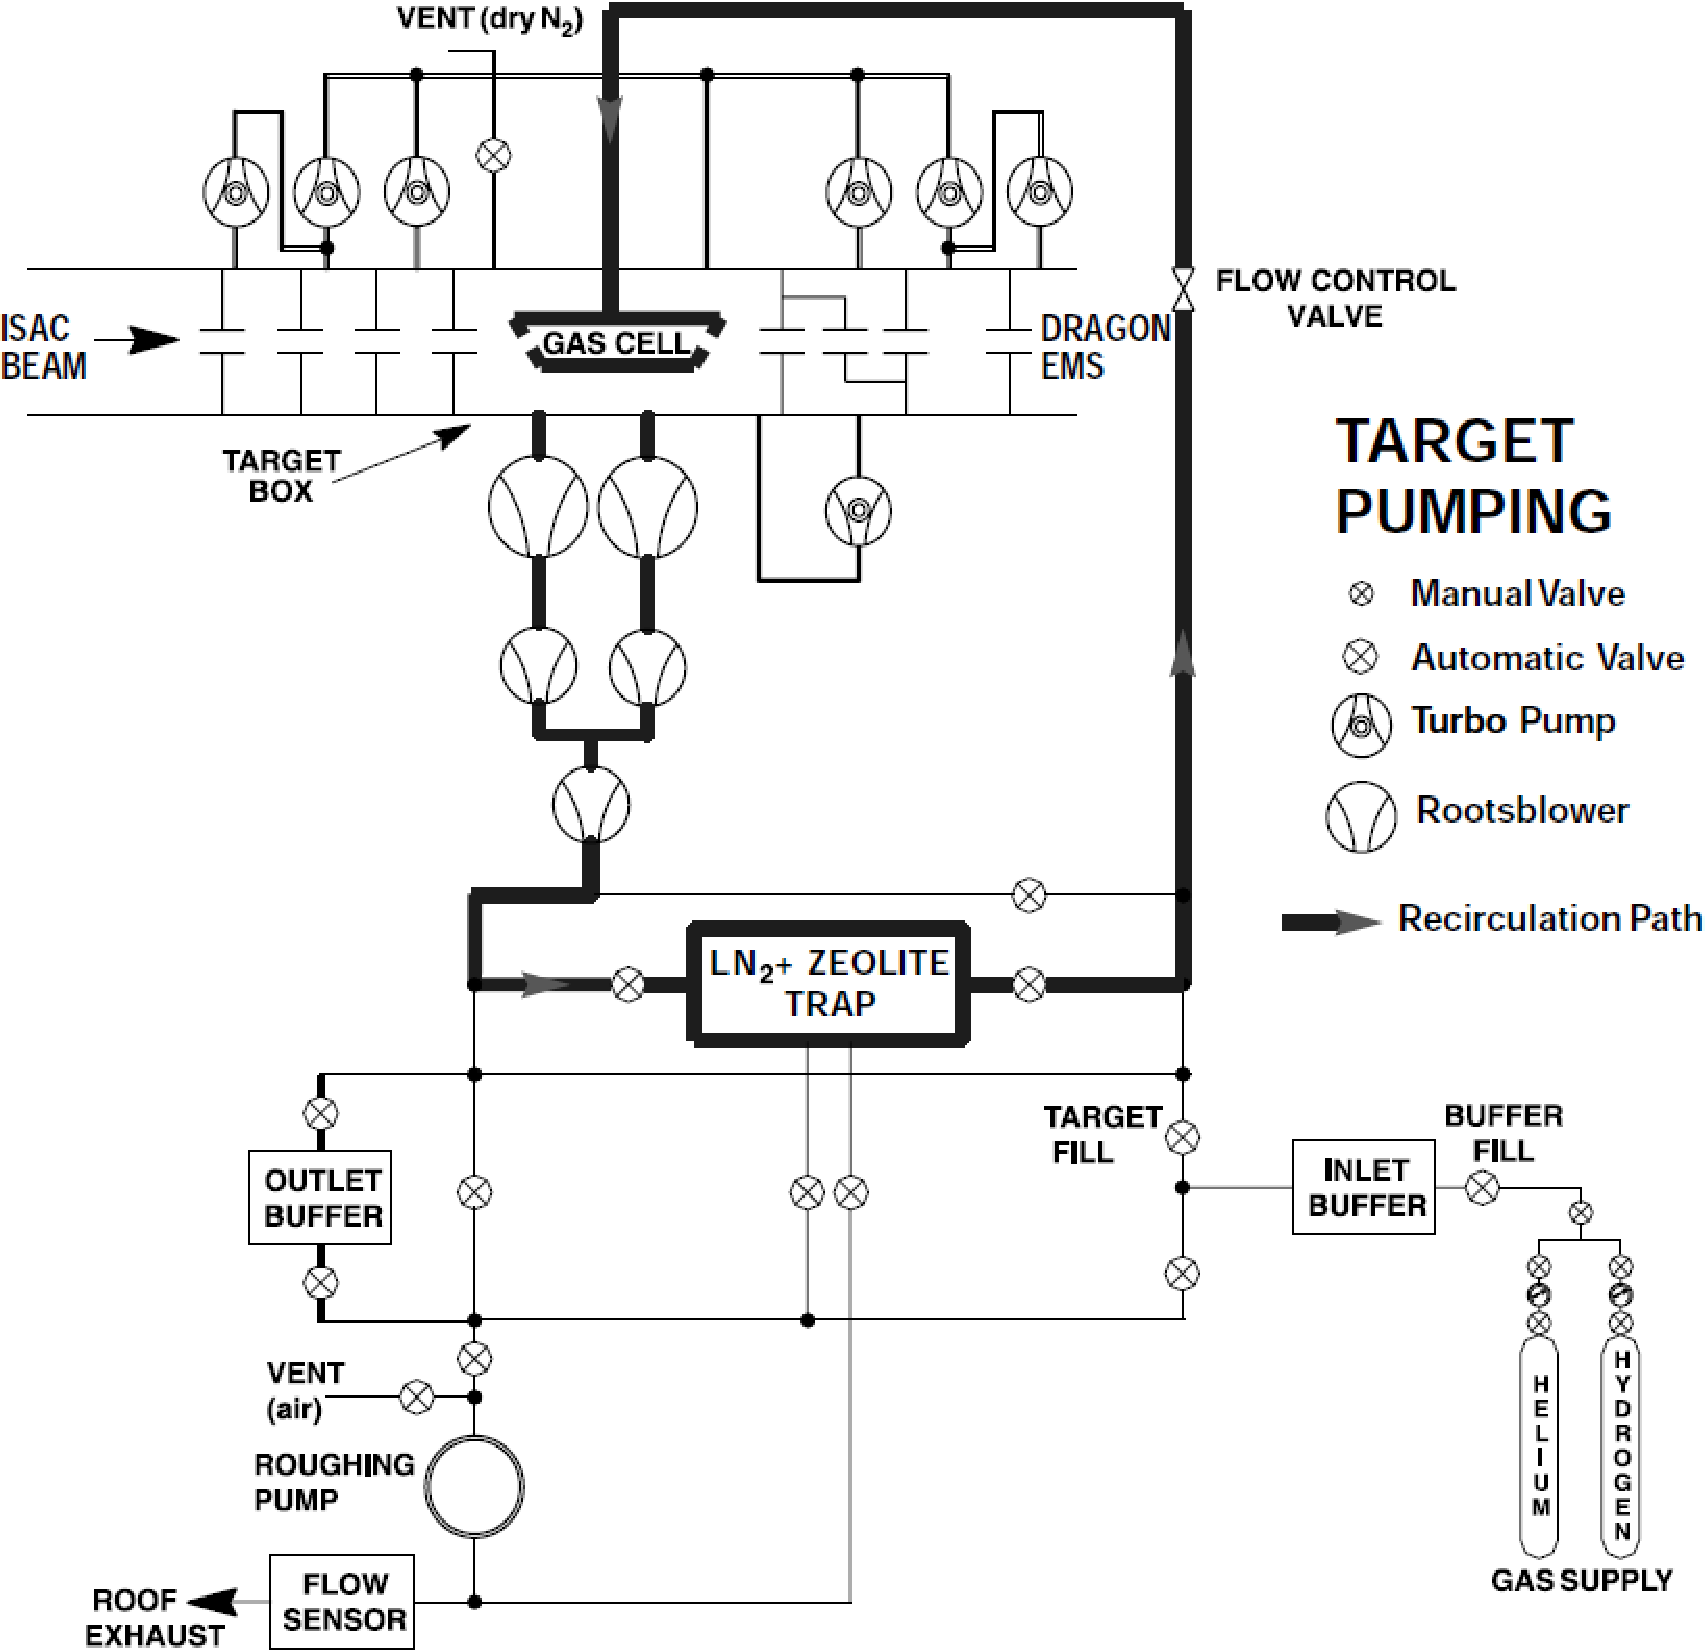
\includegraphics{Hutcheon03_Fig5_DRAGON-gastargetpumps}
}
%\vspace{5cm}       % Give the correct figure height in cm
\caption{DRAGON gas target pumping scheme. Taken from \cite{hutc03b}.}
\label{fig:dragon_pumping}
\end{figure}

%%%%%
\subsubsection{Extended length target considerations}
For the extraction of a cross section or resonance strength from the measured yield we require knowledge of the stopping power of the heavy ions in hydrogen or helium. While these are typically taken from the widely used SRIM code \cite{zieg}, recent experiments \cite{grei04} have shown deviations of the order of 20--30\% from the semi-empirical values. Therefore, direct measurement of the respective stopping power should, where possible, be preferred. This is possible when the effective length (defined as the equivalent length of constant pressure gas to achieve the same total mean ion energy loss as the non-uniform distribution) of the target is known, usually obtained through the use of a narrow-resonance reaction of known yield. 

Additionally, angle and energy scattering of the beam and recoils on their way through the target gas needs to be estimated and taken into account in the calculation of the required recoil separator acceptance. While the ions pass through the target gas they undergo charge-changing collisions. If the target is thick enough, an equilibrium charge state distribution is achieved (semi-empirical description available in {\it e.g.} \cite{liu03}). However, if the reaction recoil originates from the downstream side of the gas target, the remaining gas track length is not sufficient to reach this equilibrium, and it is advisable to obtain the charge state distribution by tuning the recoil separator for measurements of the several charge states expected to be most abundant. For reactions where the yield is spread out over the entire length of the target, e.g. direct capture, the differing charge state distribution from the non-equilibrated recoils originating from the downstream part of the target can give rise to transmission efficiency problems. Measurements of the charge state distribution at low pressures can shed some light on this, and allow models to be set up to predict the overall detection efficiency. Some detailed consideration of charge state distributions over the length of extended targets has been done in \cite{sch04} and \cite{zyl07}, for example.

An extended target also allows the interesting possibility of determining the resonance position. It has been shown in \cite{hut12} that a the reaction $\gamma$-ray hit pattern detected in coincidence with recoils can result in a determination of the resonance position with respect to the target centre. Combining this with knowledge of the effective length and the measured stopping power, this enables a quite precise way of determining resonance energy. This can be important when yields are too low to expect measurements to be made at many closely-spaced beam energies to produce an excitation function, the usual method of resonance energy determination. 


%%%%%
\subsubsection{Gas jet targets}
Especially for the astrophysically most important reactions \nuc{12}{C}\reac{\alpha}{\gamma}\nuc{16}{O} and \nuc{15}{O}\reac{\alpha}{\gamma}\nuc{19}{Ne}, the recoil cone angles are quite demanding on separator acceptance. In order not to aggravate the problem through the use of an extended gas target length of 5 -- 10 cm, recent discussions have proposed the use of a gas jet target with approximately 4 -- 5 mm jet diameter matched to the dimension of the incoming ion beam. Recent work on such a target has begun through the {\em Jet Experiments in Nuclear Structure and Astrophysics} (JENSA) collaboration, with a view to application in future facilities such as FRIB (USA) \cite{chi13}. 

As can be seen in the pumping scheme \emph{[gas jet target pumping scheme figure]} for an appropriate gas jet target ($\approx 5\times10^{18} \unit{cm^{-2}}$ areal density), such a setup (which is in its early construction phases for deployment at Oak Ridge National Laboratory) requires significantly more powerful pumping stages as well as expensive gas compression and cleaning.\\
 

%\small
%\begin{itemize} 
%\item What are the advantages of using a differentially pumped windowless gas target?
%\item for our purpose H and He targets best solution as he not available implanted in sufficient densities; H possibles but about factor 4 yield advantage due to 1/stopping term in resonant yeild equation
%\item also indestructible and stable in composition (plastic foils change and have current limit)
%\item windows are detrimental to recoil transmission, therefor windowless, differentially pumped approach ideal for our application
%\item what thickness to chooses: resonance width (usually small) + uncertainty in resonance position (info from transfer reactions plus knowledge of masses of reaction partners of order a few keV) follows target thickness of about 10 kev in CM system is useful leading areal target densities aspired of 5E18 1/cm2
%\item at 7-8 Torr achieved with about 10 cm length
%\item give equation from Rolfs for gas target density
%\item  length of target determines origin of recoil; needs to be matched with acceptance of the recoil separator (shorter is better); some reactions would benefit from gas jet which is however technically more challenging due to the large gas flow rates involved.
%\item Gas flow limiting apertures need to be matched to the heavy (radioactive) ion beam properties and the nuclear reaction recoil cone angle
%\item we need to know stopping powers; found differences to SRIM of the order of 20-30% when we measured ourselves
%\item energy and angle scattering needs to be estimated and included in acceptances; not well known
%\item charge state distributions, often equilibrium not achieved; preferably to be measured in experiment
%\end{itemize}
%\normalsize






\section{Ancillary detectors and methods}

\subsection{Beam normalisation}

All measurements of cross sections or resonance strengths require knowledge of the number of particles incident on the target. Traditionally, with the setup in normal kinematics, this is accomplished by measuring and integrating the ion beam current continuously. Alternatively, in previous inverse kinematics experiments with windowless gas targets, the thermal beam power deposited after traversing the target gas was measured in a beam calorimeter. This approach was necessary as the charge exchange in the gas passage is strongly dependent on gas pressure and beam type and energy, making a Faraday cup charge integration difficult to interpret. Another alternative pursued in the past in gas target experiments is the beam current normalization using elastic scattering of the beam ions on the target gas, which requires precise knowledge of the cross section in question. The use of recoil separators in our experiments deprives us of the possibility to pursue the first two methods as they require blockage of the ion (and recoil) beam path after the target. However, as the recoil separators purpose is to separate out the incoming ion beam, beam normalization (or diagnostic) devices can be designed to intercept all (or part, {\it e.g.} one charge state) at a location where recoils are transmitted and the beam (due to difference in mass-to-charge ratio, velocity or energy) is deposited on a selective slit. Using radioactive ion beams allows the experimenter also to monitor the radioactive decays at the locations where beam is deposited in the separator. An example of such an arrangement at the DRAGON's mass-dispersive focus is shown in Fig.\ \ref{fig:xslitm}. It allows measurement of both prompt $\gamma$ rays from the decay of radioactive beam particles stopped in the slits, and of $\beta^+$ decay via annihilation in the `horn' and subsequent detection of the coincident 511 keV $\gamma$ rays in two NaI(Tl) detectors. 
%
\begin{figure}
\centering
\resizebox{0.95\columnwidth}{!}{
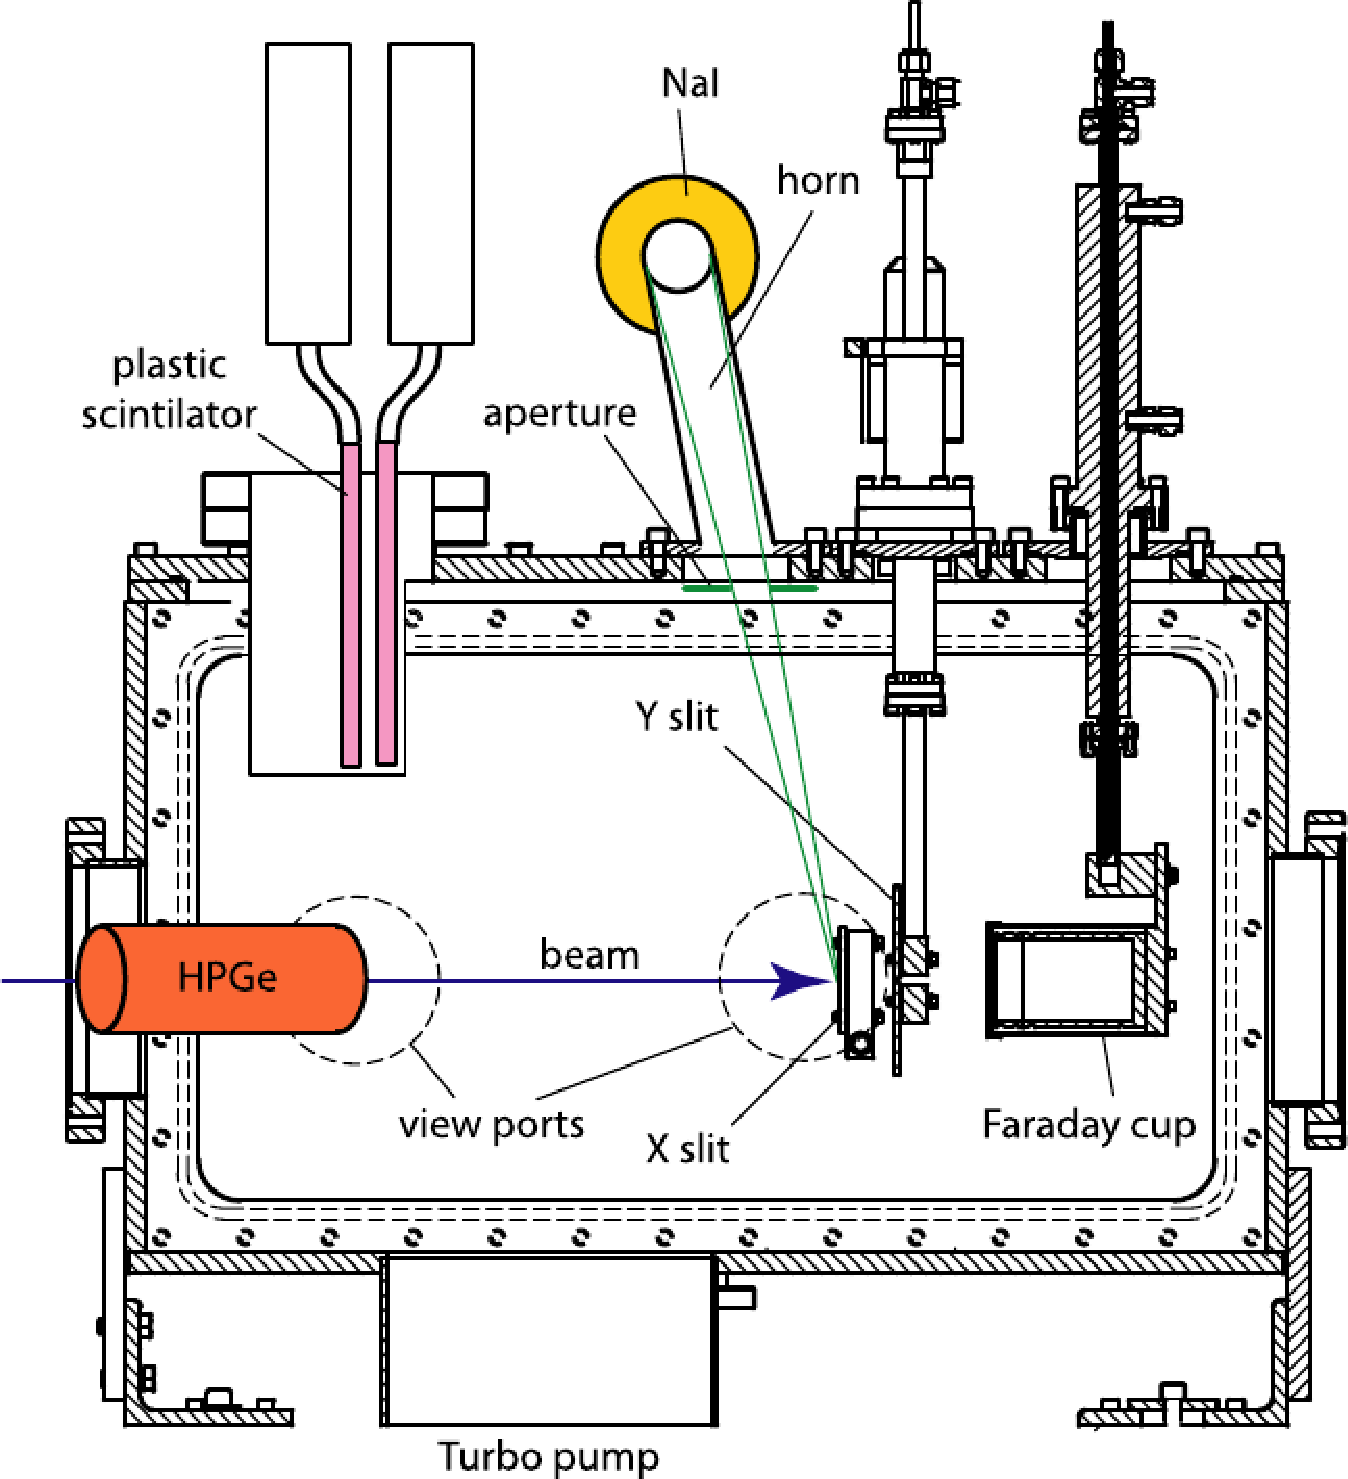
\includegraphics{Vockenhuber08_Fig3_XSLITM-chamber.pdf}
}
\caption{Radiation detectors at the DRAGON mass slits chamber. Two plastic scintillators are mounted inside a recess with a thin stainless steal wall on the side facing the mass slits. The HPGe detector (located external to the chamber) points at the mass slits through a view port, while the two NaI detectors are positioned about the `horn' and oriented at $180^\circ$ to each other. Taken from \cite{vock08}.}
\label{fig:xslitm}
\end{figure}
%
Care has to be taken, however, that different beam focussing does not affect detection efficiencies (through different deposit size or location). Additionally, the use of temporary beam intercepts is always possible, monitoring either charge or scattering in the moment of intercept, or radioactive decay of the material deposited in the non-intercept position. For example, regular Faraday cup measurements can be correlated to elastic scattering in the target, thus calibrating first the elastic scattering intensity to measured beam intensity, and subsequently normalizing the beam during the reaction measurement using the elastic scattering \cite{dau04}. 

\subsection{Prompt $\gamma$ ray detection}

Detection of prompt $\gamma$ rays by itself is a common method of determining reaction rates. $\gamma$-ray detectors are placed around a target to measure the decay lines from reaction products. This enables identification of $\gamma$ cascades and thus determination of branching ratios. This method has, however, the disadvantage of an often large background that has to be distinguished from the signal. It is thus often not possible to determine what fraction of the spectrum is due to the reaction under investigation. Combined with a recoil separator, however, prompt $\gamma$ detection at the target can be a valuable part of particle identification. $\gamma$ tagging can be used to improve the separator's background suppression by only including events with a valid $\gamma$ detection in the analysis. In conjunction with a focal plane detector, the time of flight (TOF) through the separator can be measured with the $\gamma$ event as the start signal and the focal plane detection as a stop signal (or vice versa using an appropriate delay). Using such TOF-based PID is especially advantageous when the background suppression of the separator decreases at lower energies \cite{hutc08}. 

Just as $\gamma$ tagging reduces the background in the focal plane detector, focal plane detection also reduces, and even eliminates, the background in the $\gamma$ spectrum. It is thus possible to determine the branching ratios using essentially background-free $\gamma$ spectra.\\
An additional benefit of placing $\gamma$ detectors around the target is their use in focussing the beam through the target. If the beam is poorly aligned, it can induce reactions or be deposited at the target entrance and exit aperture or on the target frame leading to increased $\gamma$ background. This background can be used as in indicator of the beam's misalignment.

Due to the typically low yields the main concern for $\gamma$ detectors in nuclear astrophysics is high efficiency. Specifically, the photo-peak efficiency needs to be high if the $\gamma$ detection is to be used to determine branching ratios. The cross section of the photo-effect varies with $\sigma_\mathrm{photo} \propto Z^{4\textrm{--}5}$, while Compton scattering goes with $\sigma_\mathrm{C} \propto Z$, and the probability for pair production as $\sigma_\mathrm{pair} \propto Z^2$. A high photo-peak efficiency therefore requires high-$Z$ materials. On the other hand, the ideal detector also has to cover a large range of energies. Reaction $Q$-values of several MeV mean that the recoil can be in states with several MeV excitation energy. Thus, a reasonable efficiency up to $\approx 10\unit{MeV}$ is required.

The fact that the $\gamma$ spectrum is essentially background free\footnote{With the exception of room background, which can be on the order of 0.1 kHz for an appropriately triggered array of BGO, for example. In addition, Coulomb-excitation of beam ions impinging on separator aperture can give rise to background $\gamma$ rays.} leads to somewhat less stringent requirements on the energy resolution. \\
The best energy resolution can be achieved using high-purity germanium (HPGe) detectors. They have, however several disadvantages. One is the relatively high cost of HPGe crystals compared to scintillator materials, another is the need for cooling, which leads to a less compact setup and additional maintenance costs. As an alternative to HPGe various scintillator materials are used for $\gamma$ detection. NaI(Tl) has a very high light output, and thus potentially good energy resolution. However, because of its low density of $3.67\unit{g/cm^3}$ it has a relatively low photopeak efficiency. In addition, it is hygroscopic, thus requiring the crystal to be sealed. Due to its high density of $7.13 \unit{g/cm^3}$, BGO (bismuth germanate) has a high photopeak efficiency. Thus, relatively small crystals can be used. Another commonly use scintillator material is BaF$_2$. Like BGO, BaF$_2$ is an intrinsic scintillator which does not require an activator. The still relatively high mass number of Ba ($Z = 56$) leads to a good photopeak efficiency. Wisshak et al. \cite{wiss84} compared the efficiencies of BGO and BaF$_2$ in an energy range from 0.5 to 10 MeV and concluded that an efficiency of 95\% would require either BGO with a thickness of 10 cm or BaF$_2$ with a thickness of 17.5 cm. Table \ref{tab:gamma_detectors} shows a comparison of some of the relevant properties of scintillation-based counters.



\begin{table*}
\label{tab:gamma_detectors}
\centering
\begin{tabular}{l|llll}
\hline
 & NaI(Tl) & BGO & BaF$_2$ & LaBr$_3$(Ce) \\
\hline
Density [$\mathrm{g/cm^3}$] & 3.67  & 7.13 & 4.88 & 5.1 \\
Hygroscopic & yes & no & slightly & yes\\
Light yield [photons/keV$\gamma$] & 38 & 8--10 & 10 (slow) & 63 \\
                                  &    &       & 1.8 (fast) &\\
Primary decay time [ns] & 250 & 300 & 630 (slow)  & 16\\
                        &     &     & 0.6 -- 0.8 (fast) &\\
\hline
\end{tabular}

\caption{Comparison of pertinent properties of various scintillation-based $\gamma$-ray detectors considered for use in recoil separators.}
\end{table*}


\subsection{Silicon strip detectors}
Silicon detectors are commonly employed as recoil detectors in the separator focal plane, their compact structure making them convenient to use. Due to the large number of charge carriers (the creation of one electron-hole pair requires 3.6 eV \cite{kemm88}) they provide good energy resolution in charged particle detection. With a pulse rise time of about 10 ns, good timing resolution is another advantage of silicon detectors, which, combined with a fast signal from {\it e.g.} a prompt $\gamma$ detector, enables precise time-of-flight measurements. \\
One disadvantage of silicon detectors is their sensitivity to radiation damage. Care must be taken not to expose them to high rates, especially of heavy particle radiation.\\
In addition to energy resolution, position resolution can be achieved by using microstrip detectors, (see Fig.\ \ref{fig:microstrip} \cite{rade84}).
%
\begin{figure}
\centering
\resizebox{0.95\columnwidth}{!}{
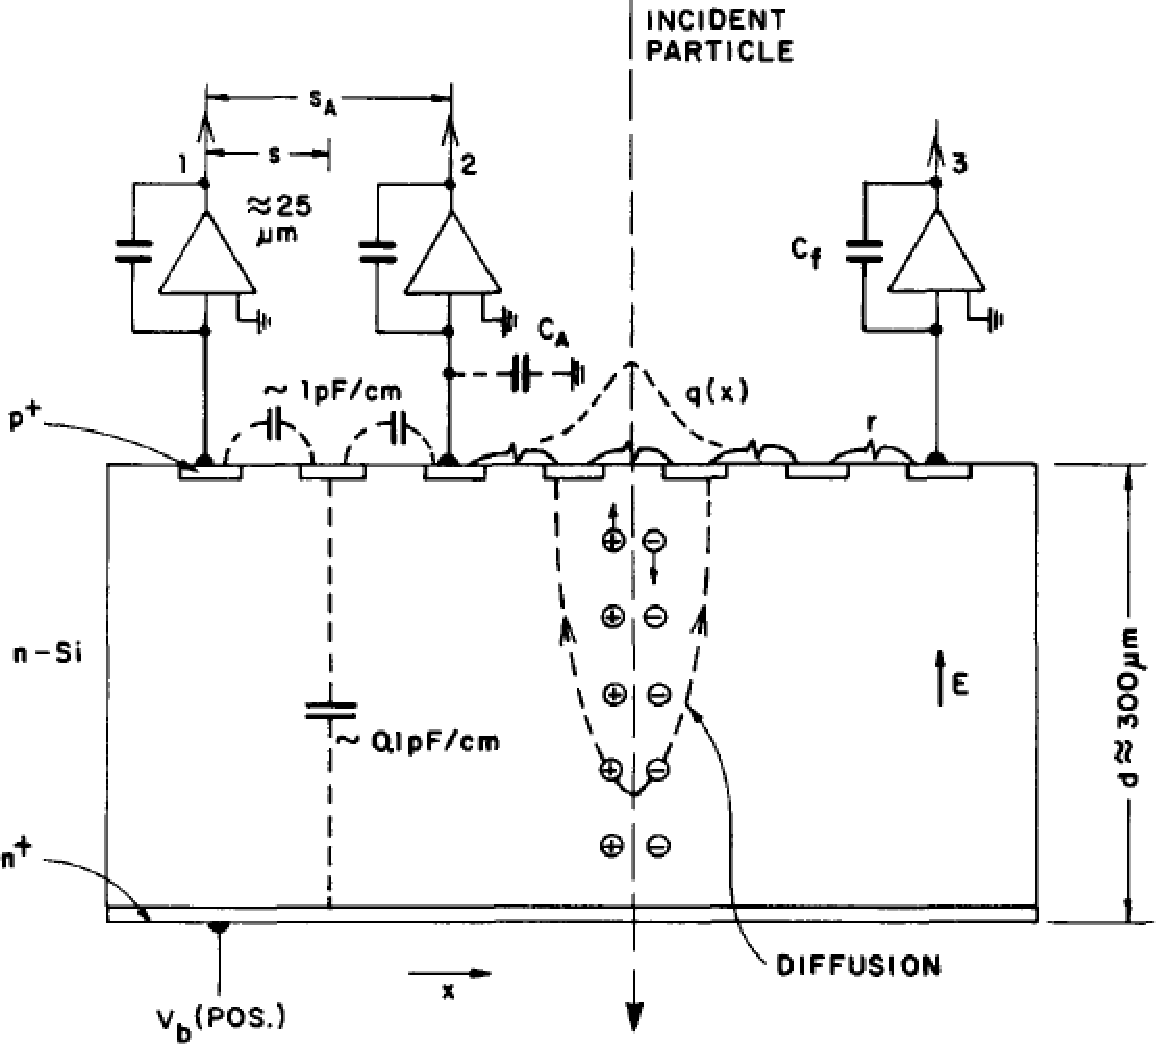
\includegraphics{Radeka84_Fig2_MicrostripDetector_PositionInterpolation.pdf}
}
\caption{Schematic representation of position interpolation in microstrip detectors. Diffusion spreads the charge [distribution $g(x)$] and determines maximum strip pitch $s$ for linear interpolation by centroid finding. Readout interpolation by capacitive charge division is illustrated between amplifiers 1 and 2. Resistive charge division is illustrated between amplifiers 2 and 3. Taken from \cite{rade84}.}
\label{fig:microstrip}
\end{figure}
%
Double-sided silicon strip detectors (DSSSDs) provide 2-dimensional position resolution by reading out perpendicular strips on the front and back of the detector. Position resolution can aid in particle identification if the recoil and the `leaky' beam follow different trajectories, but requires more electronics channels. Silicon detectors can also be stacked to form $\Delta{}E-E$ telescopes enabling particle identification by mass. However, the additional dead layers between the $\Delta{}E$ and $E$ detectors lead to a reduced energy resolution.\\  
Depending on the reaction kinematics, a $\Delta{}E-E$ telescope may require a very thin $\Delta{}E$ detector. This causes problems with mechanical stability and increases the production cost. Monolithic silicon detectors avoid this problem by integrating both detectors into one unit \cite{card96}. A thin $\Delta{}E$ layer is implanted onto a thick silicon detector. An example of such a device is shown in Fig.\ \ref{fig:monolith}, taken from Ref.\ \cite{tudi99}. Position resolution is achieved by constructing the thin layer as separate pixels, each with separate readout electronics. Thus, the number of channels required for a monolithic detector is larger than for a DSSSD. In addition, the large capacitance of the thin layer leads to a poor signal-to-noise ratio. Special preamplifiers are required to overcome this problem.%
%
\begin{figure}
\centering
\resizebox{0.95\columnwidth}{!}{
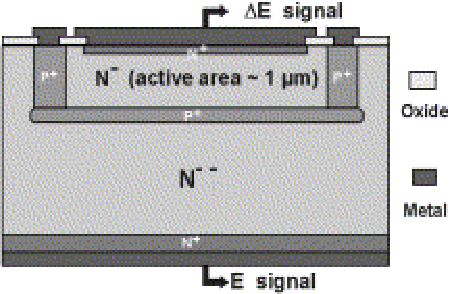
\includegraphics{Tudisco99_Fig1_monolith_sideview}
}
\caption{Side view of a monolithic silicon detector. Taken from \cite{tudi99}.}
\label{fig:monolith}
\end{figure}
%

\subsection{Ionization chambers}
At low energies ionization chambers (ICs) can be advantageous compared to silicon detectors, since a thin dead layer can be achieved by using an appropriately thin window. At such energies, the pressure inside the IC can be low while still stopping the particle in the active volume, allowing for the use of a thin window of sufficient size. Another advantage is that ICs are relatively low cost and, due to the lack of a solid structure, resistent to radiation damage.\\
The anode of an IC may be segmented, thus providing $\Delta{}E-E$ (often with several $\Delta{}E$ stages) particle identification. While the gas pressure can be adjusted to fit the beam and reaction product and their respective stopping powers, and thus optimise the resolution, the energy resolution is still inferior to that of a silicon detector. This is largely due to the lower number of charge carriers created by the incident particle; in most common gases, the energy required to create an electron-ion pair is about 25 -- 45 eV/pair (compare to 3.6 eV per electron-hole pair in silicon).\\
The timing resolution depends on the drift time of the electrons to the anode, which in turn depends on the geometry of the chamber, the drift gas, and the applied voltages. The drift time is usually of the order of $\unit{\mu{}s}$, leading to a timing resolution inferior to that of silicon detectors. 
ICs are in use at several recoil separator facilities. The DRAGON IC is shown in Fig.\ \ref{fig:ICs}. In this case, not only can the gas pressure be adjusted, but the widths of the anodes can be changed in steps of 1 cm, using up to 5 anodes total.
Alternatively, with an unsegmented anode, the IC can function as a $\Delta{}E$ stage with a silicon detector mounted at the back as the $E$ detector. Such a setup was used, {\it e.g.} at ARES \cite{coud03}, and is shown in the top panel of Fig.\ \ref{fig:ICs}.
\begin{figure}
\centering
\resizebox{0.8\columnwidth}{!}{%
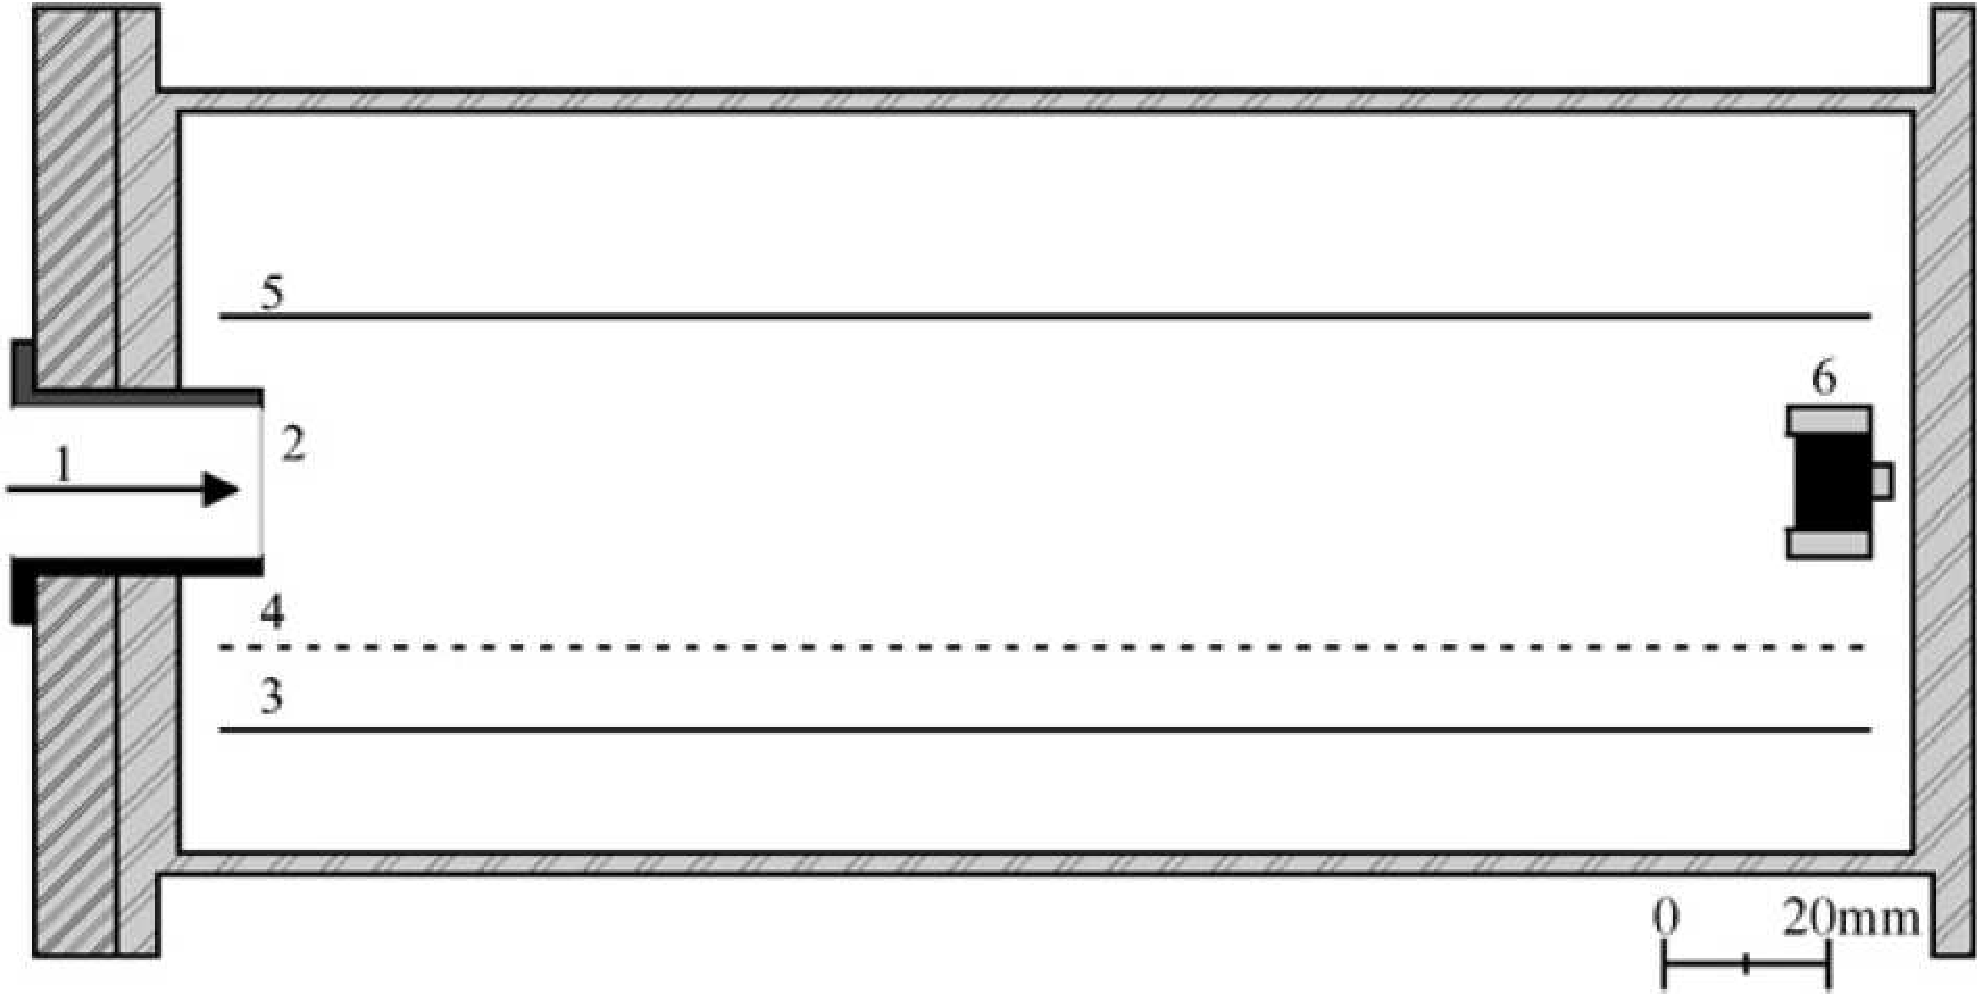
\includegraphics{Couder03_Fig5_ARES-IC}
}
\resizebox{0.98\columnwidth}{!}{%
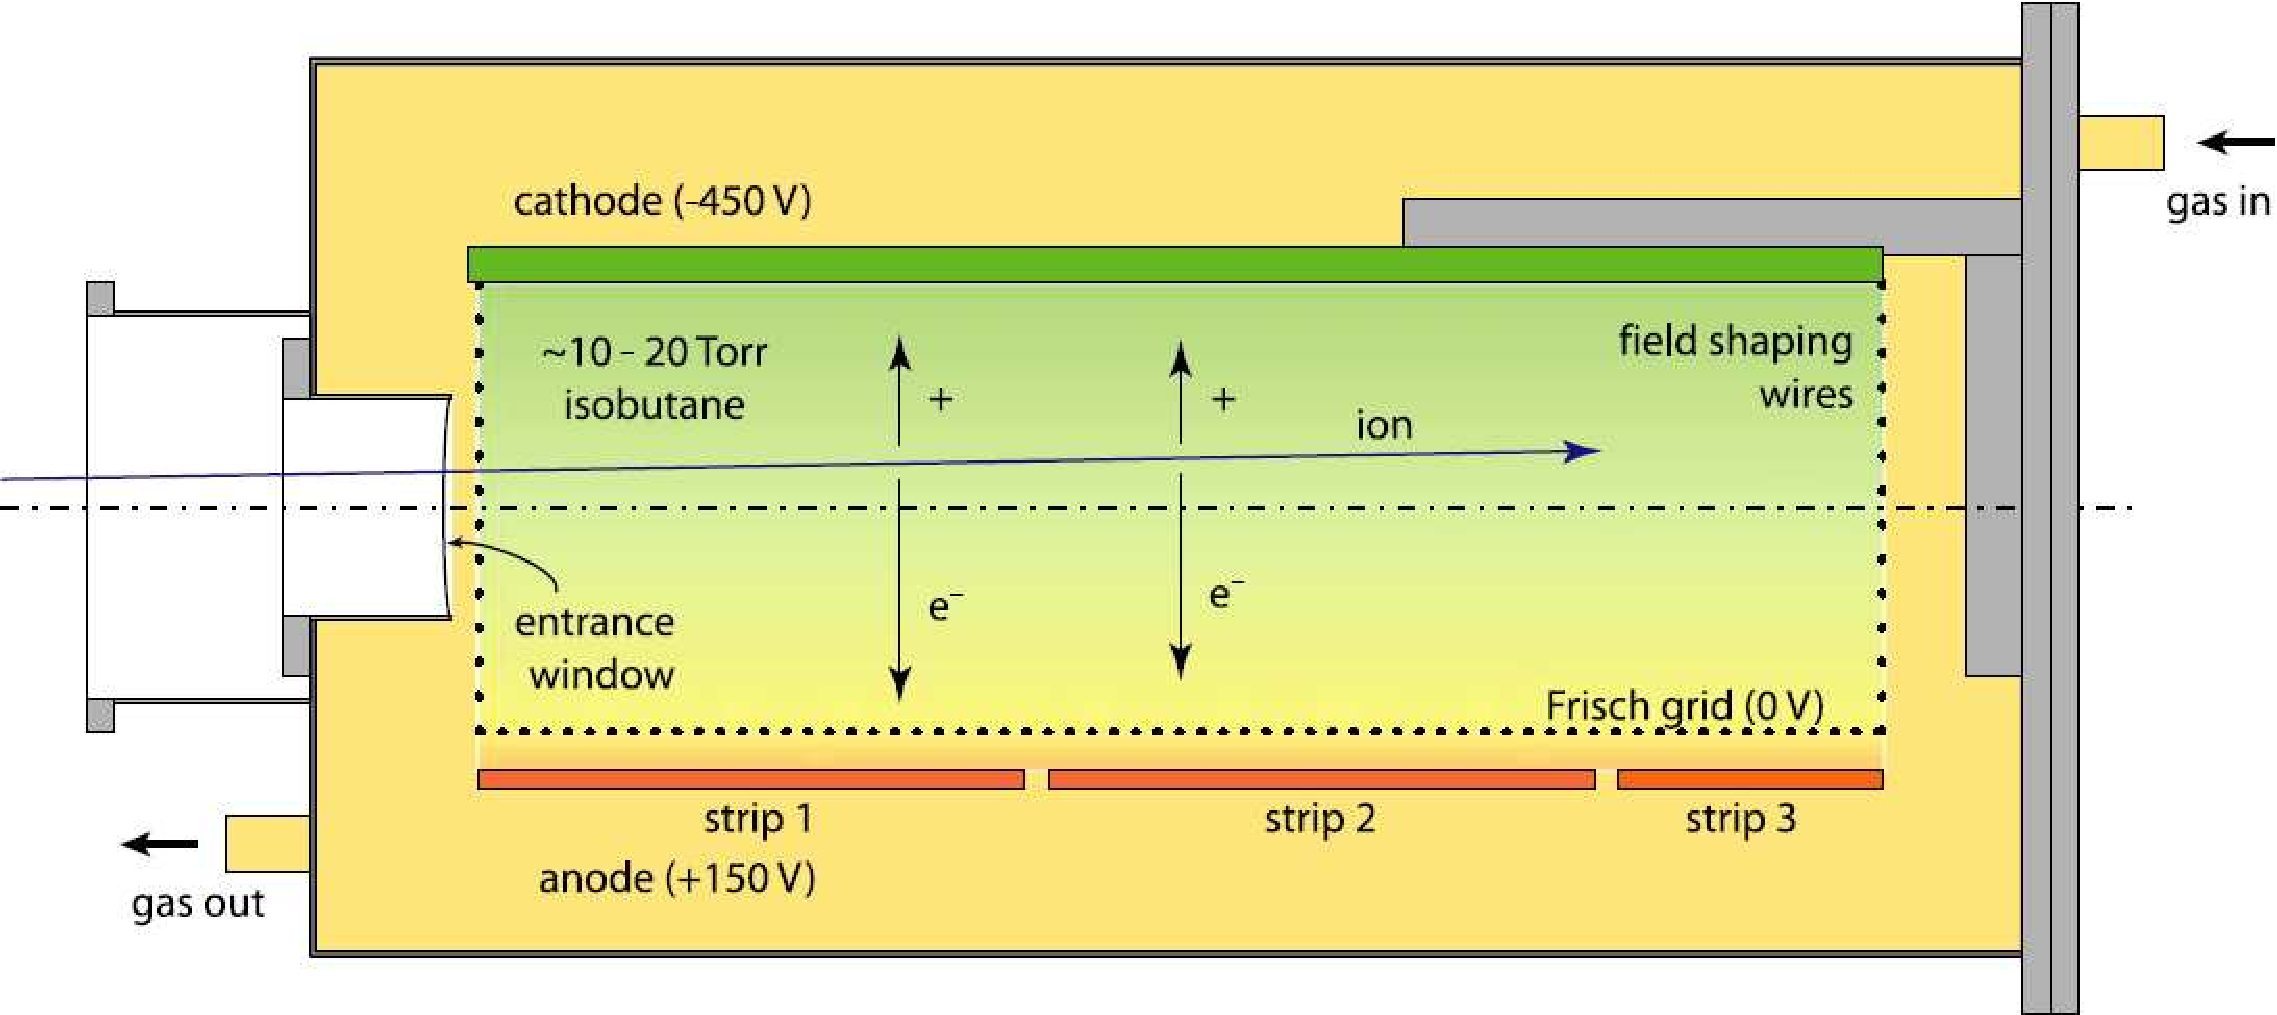
\includegraphics{Vockenhuber08_Fig4_DRAGON-IC}
}
\caption{Drawings of the ARES (upper) and DRAGON (lower) ICs. Taken from \cite{coud03,vock08}.}
\label{fig:ICs}
\end{figure}


\subsection{Local time-of-flight}

Non-destructive time-of-flight measurement provides good resolution at lower energies, where the IC and DSSSD resolutions decrease. This is especially important as the beam suppression of the separator generally decreases with decreasing energy \cite{hutc08}. The advantage of a non-destructive measurement is that it can be combined with PID in a focal plane detector. The measurement should thus interfere as little as possible with the particles' energy and trajectory. In addition, the resolution must be sufficient to distinguish reaction recoils from beam particles. From this follow requirements for the detectors' timing resolution and hence the minimum distance between them. In typical \reac{p}{\gamma} and \reac{\alpha}{\gamma} reactions in nuclear astrophysics, the recoil velocity is usually between 75 and 95\% of the beam velocities, with beam velocities of around $10^7 \unit{m/s}$.   \\
One way to meet the requirements is to use microchannel plate (MCP) detectors to detect secondary electrons emitted when the beam passes through a thin foil \cite{star82}. The secondary electrons can be deflected into the MCP using wire planes at appropriate potentials, as shown in Fig. \ref{fig:Starzecki82_Fig1}.
%
\begin{figure}
\centering
\resizebox{0.98\columnwidth}{!}{
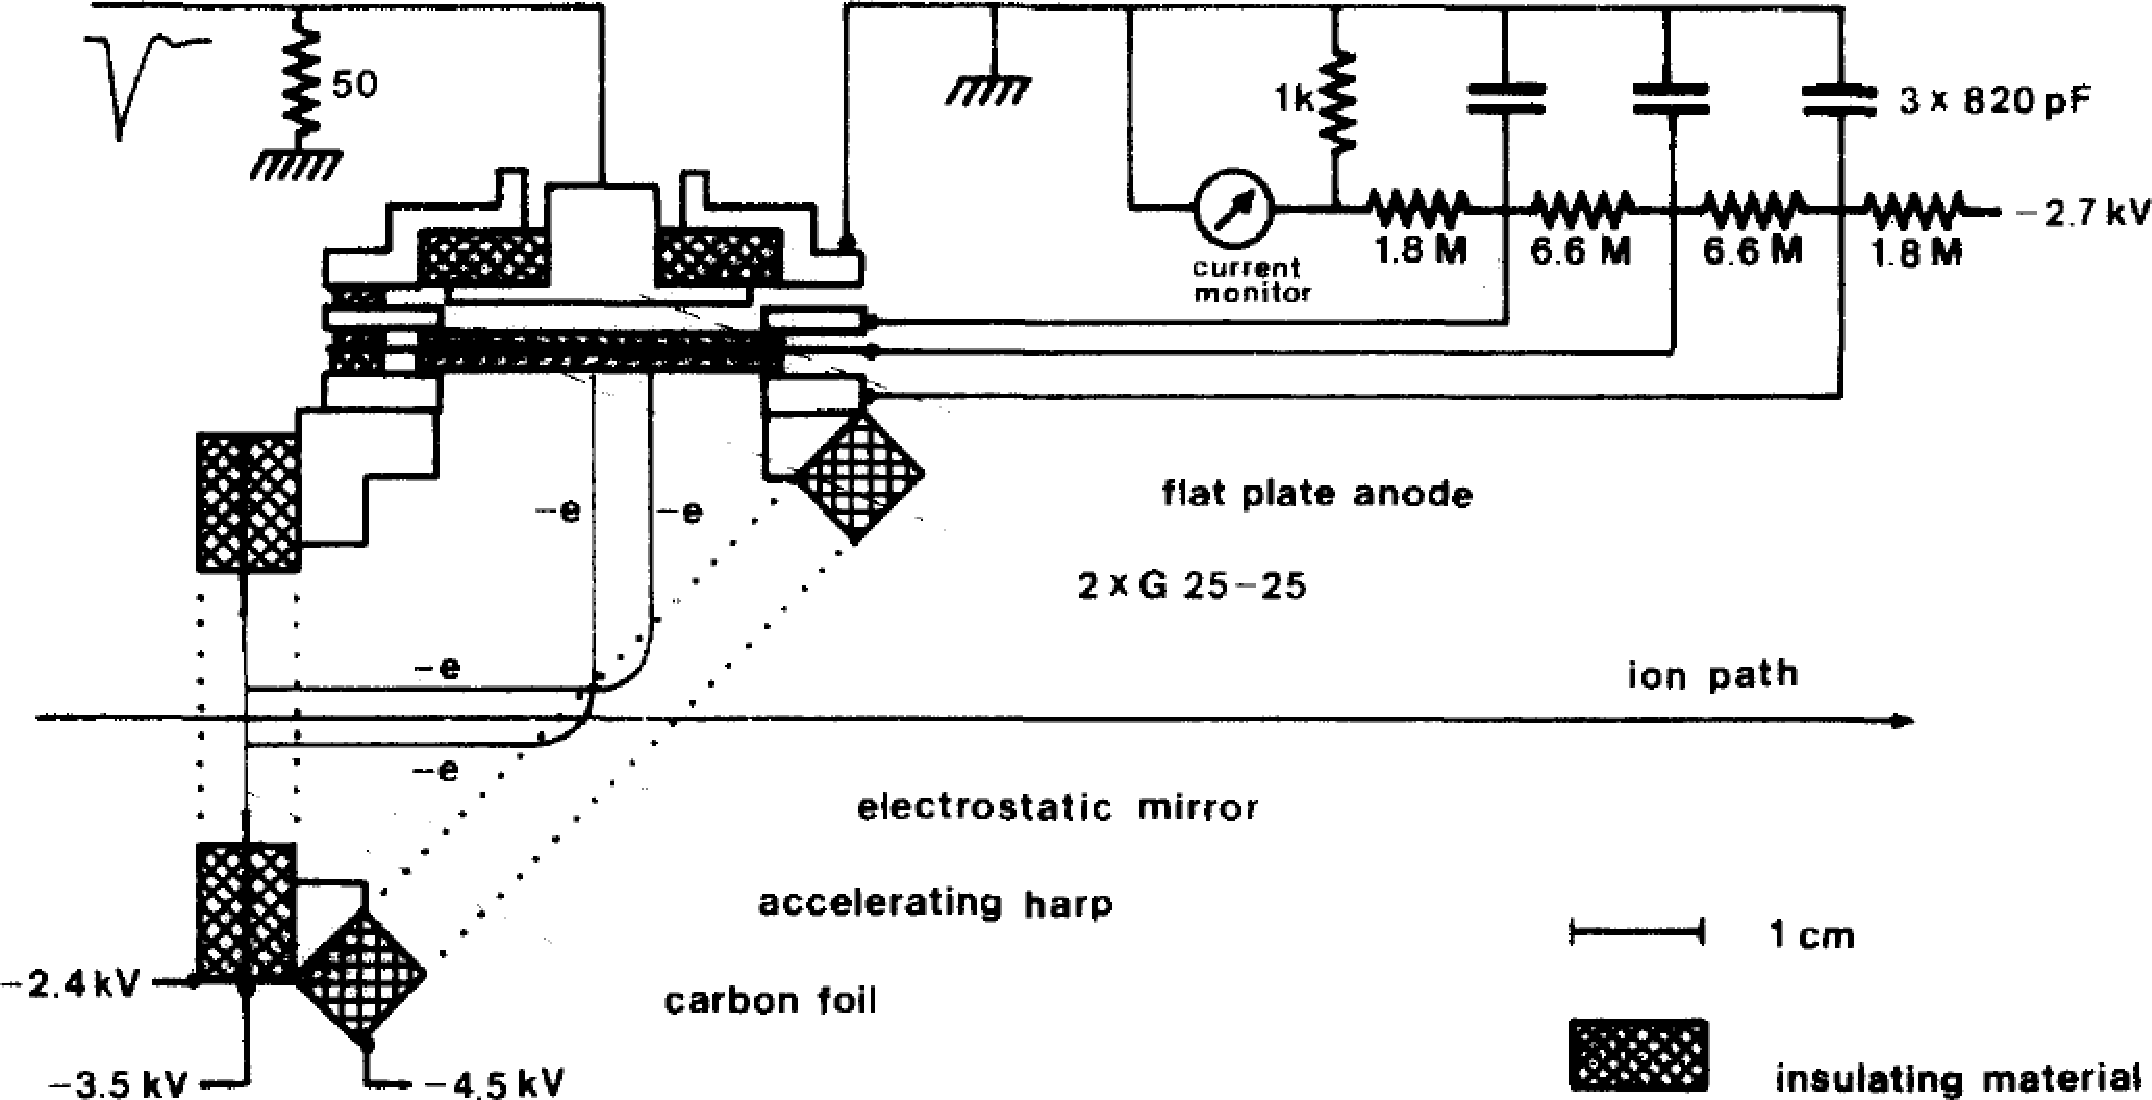
\includegraphics{Starzecki82_Fig1_TimeZeroDetector.pdf}
}
\caption{Schematic view of the time-zero detector. With the potentials indicated here the reflection of the electrons occurs 1.5 mm inside the mirror. Taken from \cite{star82}.}
\label{fig:Starzecki82_Fig1}
\end{figure}%
%
The MCP itself can thus be mounted outside the beam path. MCP detectors have a very good timing resolution of around 100 ps. They can also be build using resistive anodes and thus enabling position measurement. If the trajectories of the reaction products and the beam particles differ, this position can be used as an additional PID parameter. Using two such setups separated by 59 cm, timing resolutions of better than 400 ps have been demonstrated \cite{vock09}. \\
The efficiency of the foil-MCP system depends on how many secondary electrons are emitted from the foil when the charged particle passes through. This number depends on the stopping power $dE/dx$ and is thus larger for heavier ions. In addition, the electron multiplication in the MCP and the electronic threshold influence the detection efficiency.\\
The thickness of the foils is limited by the required energy resolution in the focal plane detector. Thinner foils are desirable, but difficult to float on frames with large apertures, which are required to cover the different trajectories of recoil ions and scattered beam. Thus, the foils are often mounted on meshes \cite{vock09}. Still, pin-holes can cause reduction in the detection efficiency. The meshes also reduce the transmission of the TOF system, as do the electrostatic mirror wire planes. 


       % Ancillary detectors and methods 

\section{Early and recent work at stable beam facilities}

\subsection{Caltech separator}

With the availability of heavy ion beams at energies which would allow radiative capture measurements in inverse kinematics, windowless gas targets were developed, which in several experiments showed an improved $\gamma$ detection environment due to a reduction in beam induced backgrounds. However, as nuclear astrophysics experiments usually need to push the boundaries of the possible to reach the astrophysically relevant energy regimes (associated with low experimental yields), it was quickly realized that the small recoil cone angle associated with the emission of a radiative capture $\gamma$ ray would allow efficient reaction recoil detection for further background suppression through a coincidence requirement. The concept was first realized at the California Institute of Technology (Caltech) in the middle of the 1980's. The Caltech set-up used a heavy ion beam from the 3 MV Pelletron Tandem Accelerator at the Kellogg Radiation Laboratory. It consisted of a windowless, differentially pumped (two sided) gas target and a recoil separator using two separation stages, Fig. \ref{fig:caltech}.

\begin{figure}
\centering
\resizebox{0.8\columnwidth}{!}{
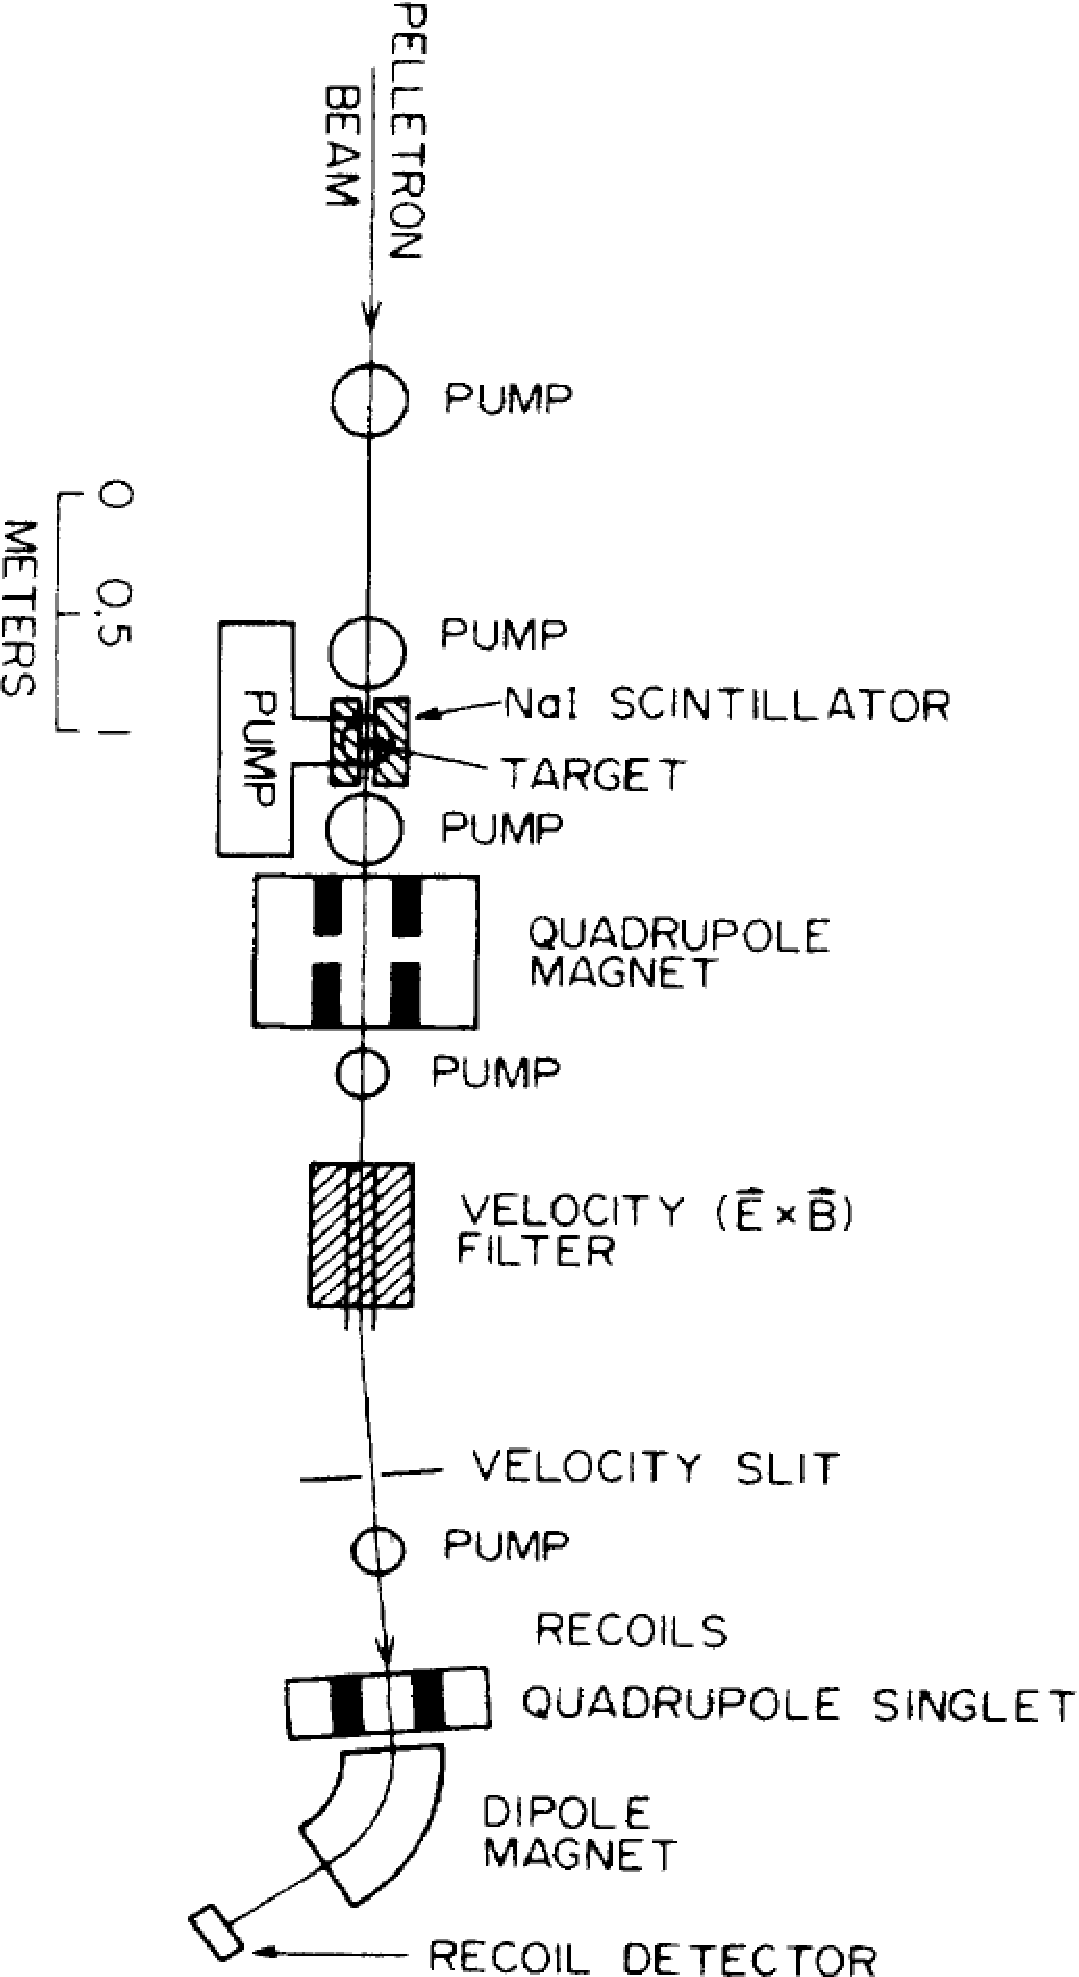
\includegraphics{Hahn87_Fig2_CaltechSeparator}
}
%\vspace{5cm}       % Give the correct figure height in cm
\caption{Schematic view of the Caltech separator. Taken from \cite{hahn87}.}
\label{fig:caltech}       % Give a unique label
\end{figure}

Immediately after emerging from the last pumping stage of the gas target (through conical gas flow limiters), the recoil cone was re-focussed by a quadrupole doublet onto a variable slit. Velocity filtering employing this slit was provided by a Wien filter. Such an element transmits all charge states of a given velocity, and further cleanup of the recoils to the focal plane is provided by a dipole magnet through momentum and charge state selection. The transmitted recoils and `leaky' beam particles were detected with a two segment ionization chamber (IC) using $Z$-identification through the difference in energy loss. Additionally, a parallel grid proportional counter (PGAC) preceded the IC in a separate gas volume to provide a timing signal. The arrival of a particle at the end of the recoil separator provided the logical condition for an array of four large NaI detectors to allow recording of a possible $\gamma$ signal with over 50\% efficiency.

The Caltech separator was built for the measurement of those alpha radiative capture reactions most relevant to stellar helium burning. In the important energy regime, cross sections of below $1 \unit{nb}$ and recoil cones above 15 mrad were expected. The setup was used for two published experiments: the design benchmark \nuc{12}{C}\reac{\alpha}{\gamma}\nuc{16}{O} \cite{krem88} and a determination of the direct capture component of \nuc{16}{O}\reac{\alpha}{\gamma}\nuc{20}{Ne} \cite{hahn87}. In both experiments, the recoil separator provided a beam suppression of the order of $10^8$ to $10^9$. The maximum count rate permissible in the focal plane detectors ($\approx 30 \unit{kHz}$) limited the beam current to be employed to a few micro-Ampere. At these high count rates a reliable reaction detection through evaluation of only the recoils in the focal plane was not attempted, instead the recoil detection was used as a trigger for the NaI $\gamma$ detector array. Although the available publications state no precise maximum acceptance numbers for the Caltech separator experiments, they reveal that for the \nuc{12}{C}\reac{\alpha}{\gamma}\nuc{16}{O} reaction only part of the reaction recoils could be transmitted, while the \nuc{16}{O}\reac{\alpha}{\gamma}\nuc{20}{Ne} reaction ($\frac{\Delta{}v}{v} \approx 2 \%$) recoil cone (due to the smaller $Q$-value) fit comfortably. Ray-trace simulation allowed cross sections down to the $0.2 \unit{nb}$ range to be extracted from the experiments.\\ 
These pioneering measurements revealed clearly both the advantages and disadvantages of the recoil detection approach. The use of the recoil separator allowed the recording of background free $\gamma$ spectra. However, the available beam suppression factor limited the amount of beam current usable to the count rate capabilities of the focal plane detection system. Additionally, the dependence of recoil transmission on the $\gamma$ ray energy and emission angle, in this case of limited recoil cone acceptance, does not allow truly independent measurements. In the time period of the above cited measurements, discussions started about the realization of radioactive ion beam facilities. In the area of nuclear astrophysics radioactive ion beam measurements to elucidate the hot CNO cycle were perceived to be a primary aim. It was quickly realized that for the necessary proton radiative capture experiments the recoil separator approach would be ideal. In order to explore the usefulness of the existing Caltech setup for these types of projected experiments Smith {\it et al.} \cite{smit91} performed a series of measurements of the \nuc{12}{C}\reac{p}{\gamma}\nuc{13}{N} reaction focussing on direct \nuc{13}{N} recoil detection. Comparison of direct $\gamma$ capture yield, \nuc{13}{N} capture/activity determination, and \nuc{13}{N} direct recoil detection methods produced reliable results within errors proving the feasibility of the recoil separator approach. The collaborators on this experiment suggested the use of additional filter elements and/or baffles to improve the performance of future dedicated recoil separators at radioactive ion beam facilities. Additionally, they called for work on the improvement of focal plane detectors to allow better recoil identification. It is worth noting that the measurement of the DC component of the \nuc{16}{O}\reac{\alpha}{\gamma}\nuc{20}{Ne} at the Caltech separator \cite{hahn87} is probably the smallest reaction cross section that has ever been measured at a recoil facility at on the order of 1 \unit{nb}, closely followed by various measurements of \nuc{12}{C}\reac{\alpha}{\gamma}\nuc{16}{O} (based on coincident recoil detection only without separation of multipole components using $\gamma$ ray data). 

\subsection{NABONA}

The first experiment attempting to measure radiative proton capture on a radioactive nucleus using a recoil separator was performed at a stable ion beam facility. In this case, like in many of the early nuclear astrophysics recoil separator setups, a set of existing beam line components (here from an accelerator mass spectrometry experiment) was adapted for the measurements. The goal of this effort was to determine the absolute cross section of radiative proton capture on \nuc{7}{Be}, which is a crucial reaction for predicting the neutrino spectrum emanating from our sun. In order to be competitive with previous efforts using a solid \nuc{7}{Be} target (which were possible due to the relatively long half-life of 52.9 days) the setup was designed to keep systematical errors at the 5\% level. This condition influenced the design of the windowless gas target, which, at a length of about 15 cm, was a factor three longer than the Caltech setup (and allowed for twice the gas cell pressure). However, the low $Q$-value of the \nuc{7}{Be}\reac{p}{\gamma}\nuc{8}{B} reaction results in a much smaller recoil cone than the alpha captures targeted at Caltech. At the NApoli-BOchum-Nuclear Astrophysics (NABONA) setup the acceptance was clearly available to provide full transmission for a selected recoil charge state. The Universita Federico II in Napoli, Italy, operates a 3 MV tandem accelerator, equipped with a sputter ion source, which was supplied with a \nuc{7}{Be} (produced at the ATOMKI, Hungary) sputter cathode. After momentum and charge analysis (selecting the $4^+$ charge state to suppress \nuc{7}{Li} beam components) the \nuc{7}{Be} beam was guided through the windowless gas target. In the NABONA approach, a dipole magnet was used first to select one charge state of both beam and recoils on a focus (achieved by a quadrupole doublet) through a pair of slits, see Fig. \ref{fig:nabona}.\\
\begin{figure*}
\begin{center}
\resizebox{1.5\columnwidth}{!}{
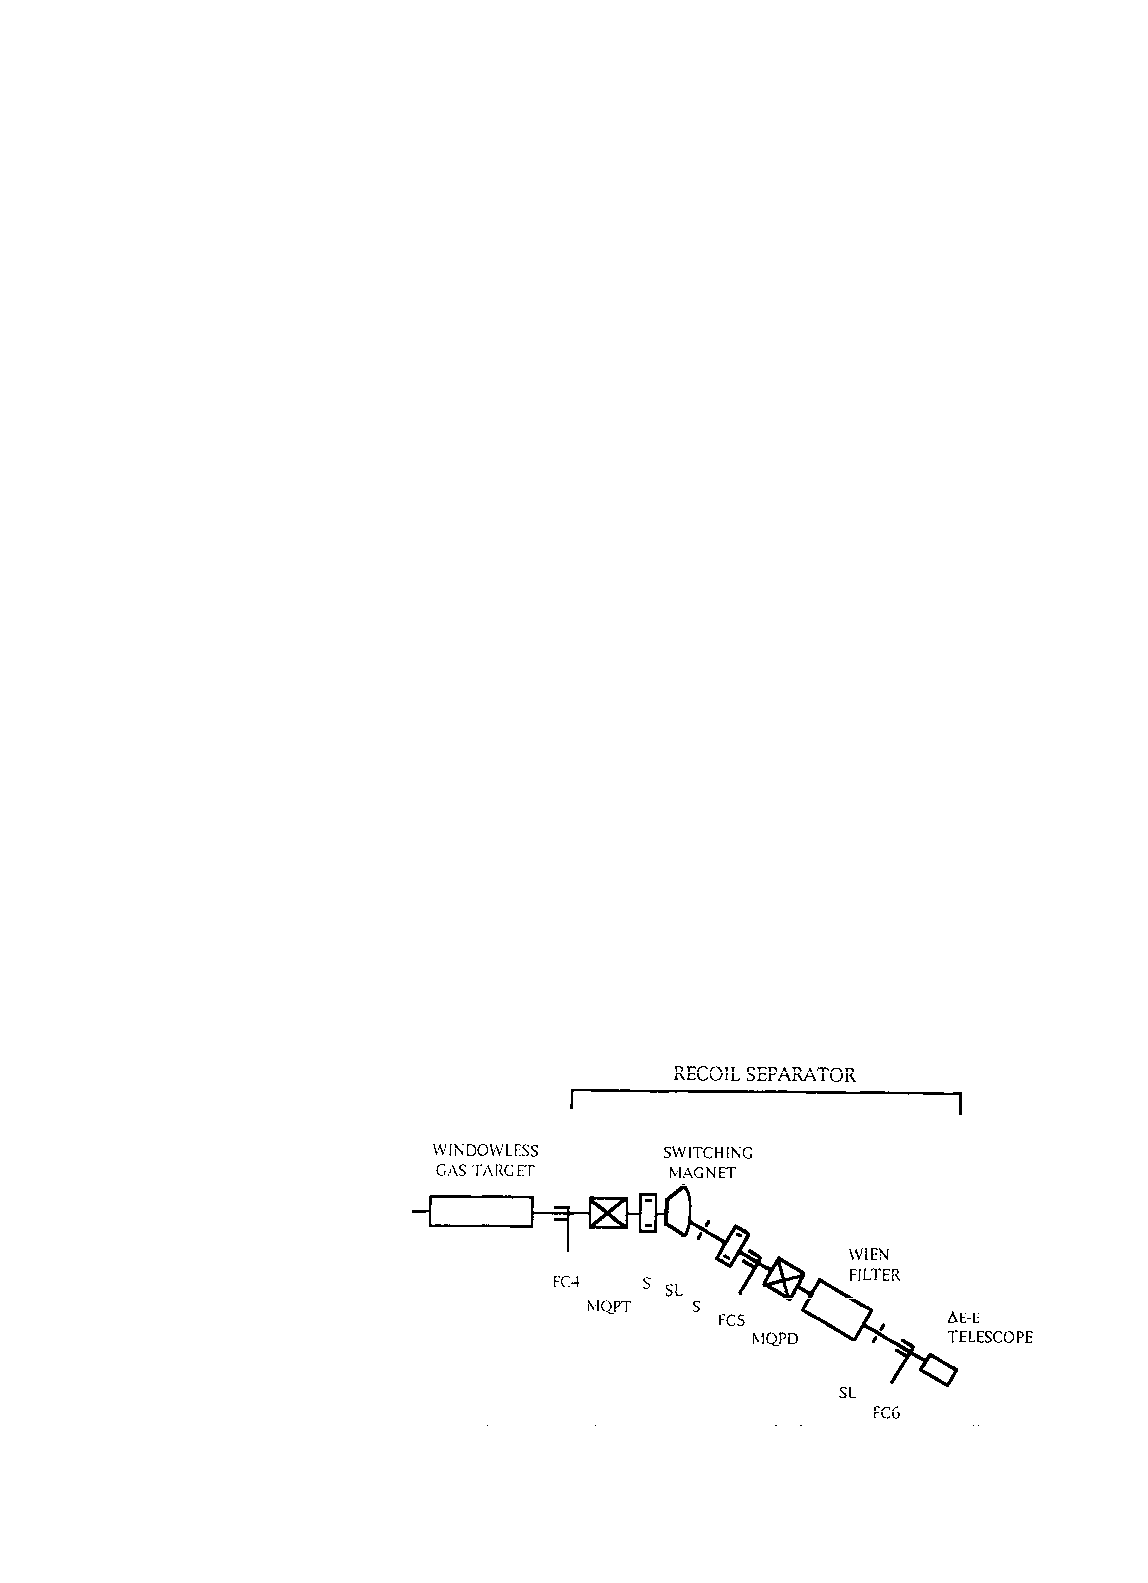
\includegraphics{Gialanella96_Fig1_NABONA}
}
\caption{Schematic view of the NABONA separator. Taken from \cite{gial96}.}
\label{fig:nabona}
\end{center}
\end{figure*}
After traversing the charge selecting slits, another quadrupole focussed the ions towards the final focal plane. On the way, they passed a crossed-field (Wien-) velocity filter, which was set to allow passage only for reaction recoils (beam and recoils have the same momentum, but differ in velocity). At the end of the separator, a two section $\Delta{}E$-$E$ ionization chamber provided recoil identification. The complete setup was tested carefully \cite{gial96}, using again the \nuc{12}{C}\reac{p}{\gamma}\nuc{13}{N} reaction to establish that the momentum distribution (also causing the recoil cone) of the \nuc{7}{Be}\reac{p}{\gamma}\nuc{8}{B} target reaction would fit into its acceptance. The observed value for $\frac{\Delta{}p}{p}$ amounted to $\approx1.9\%$ at slit settings which provided an incident \nuc{12}{C} beam suppression of $2\cdot10^{-10}$. The choice of gas flow limiting apertures allowed acceptance of recoils emerging within a cone of half-angle $0.4^\circ$. The resulting cross section measured for the \nuc{12}{C}\reac{p}{\gamma}\nuc{13}{N} reaction agreed well with literature values. It should be noted that this separator was the first to be designed to function without the coincidence condition from a $\gamma$ detector array around the gas target region. Beam suppression from the electromagnetic elements in conjunction with focal plane detection was sufficient to provide unambiguous  recoil identification. It appeared in comparison to the Caltech separator, which basically used the same types of filtering elements, that the early selection of just one charge state for transport was beneficial for the improvement of the beam suppression factor. 

\subsection{ERNA}

The lessons learned from the NABONA project were useful to the same collaboration in the start of a similar project at the Bochum Dynamitron Tandem accelerator laboratory. The European Recoil separator for Nuclear Astrophysics (ERNA) was built using components of the Caltech separator, modified for larger acceptance and supplemented with additional large bore quadrupoles and crossed-field (Wien-) filters.
\begin{figure*}
\begin{center}
\resizebox{1.8\columnwidth}{!}{
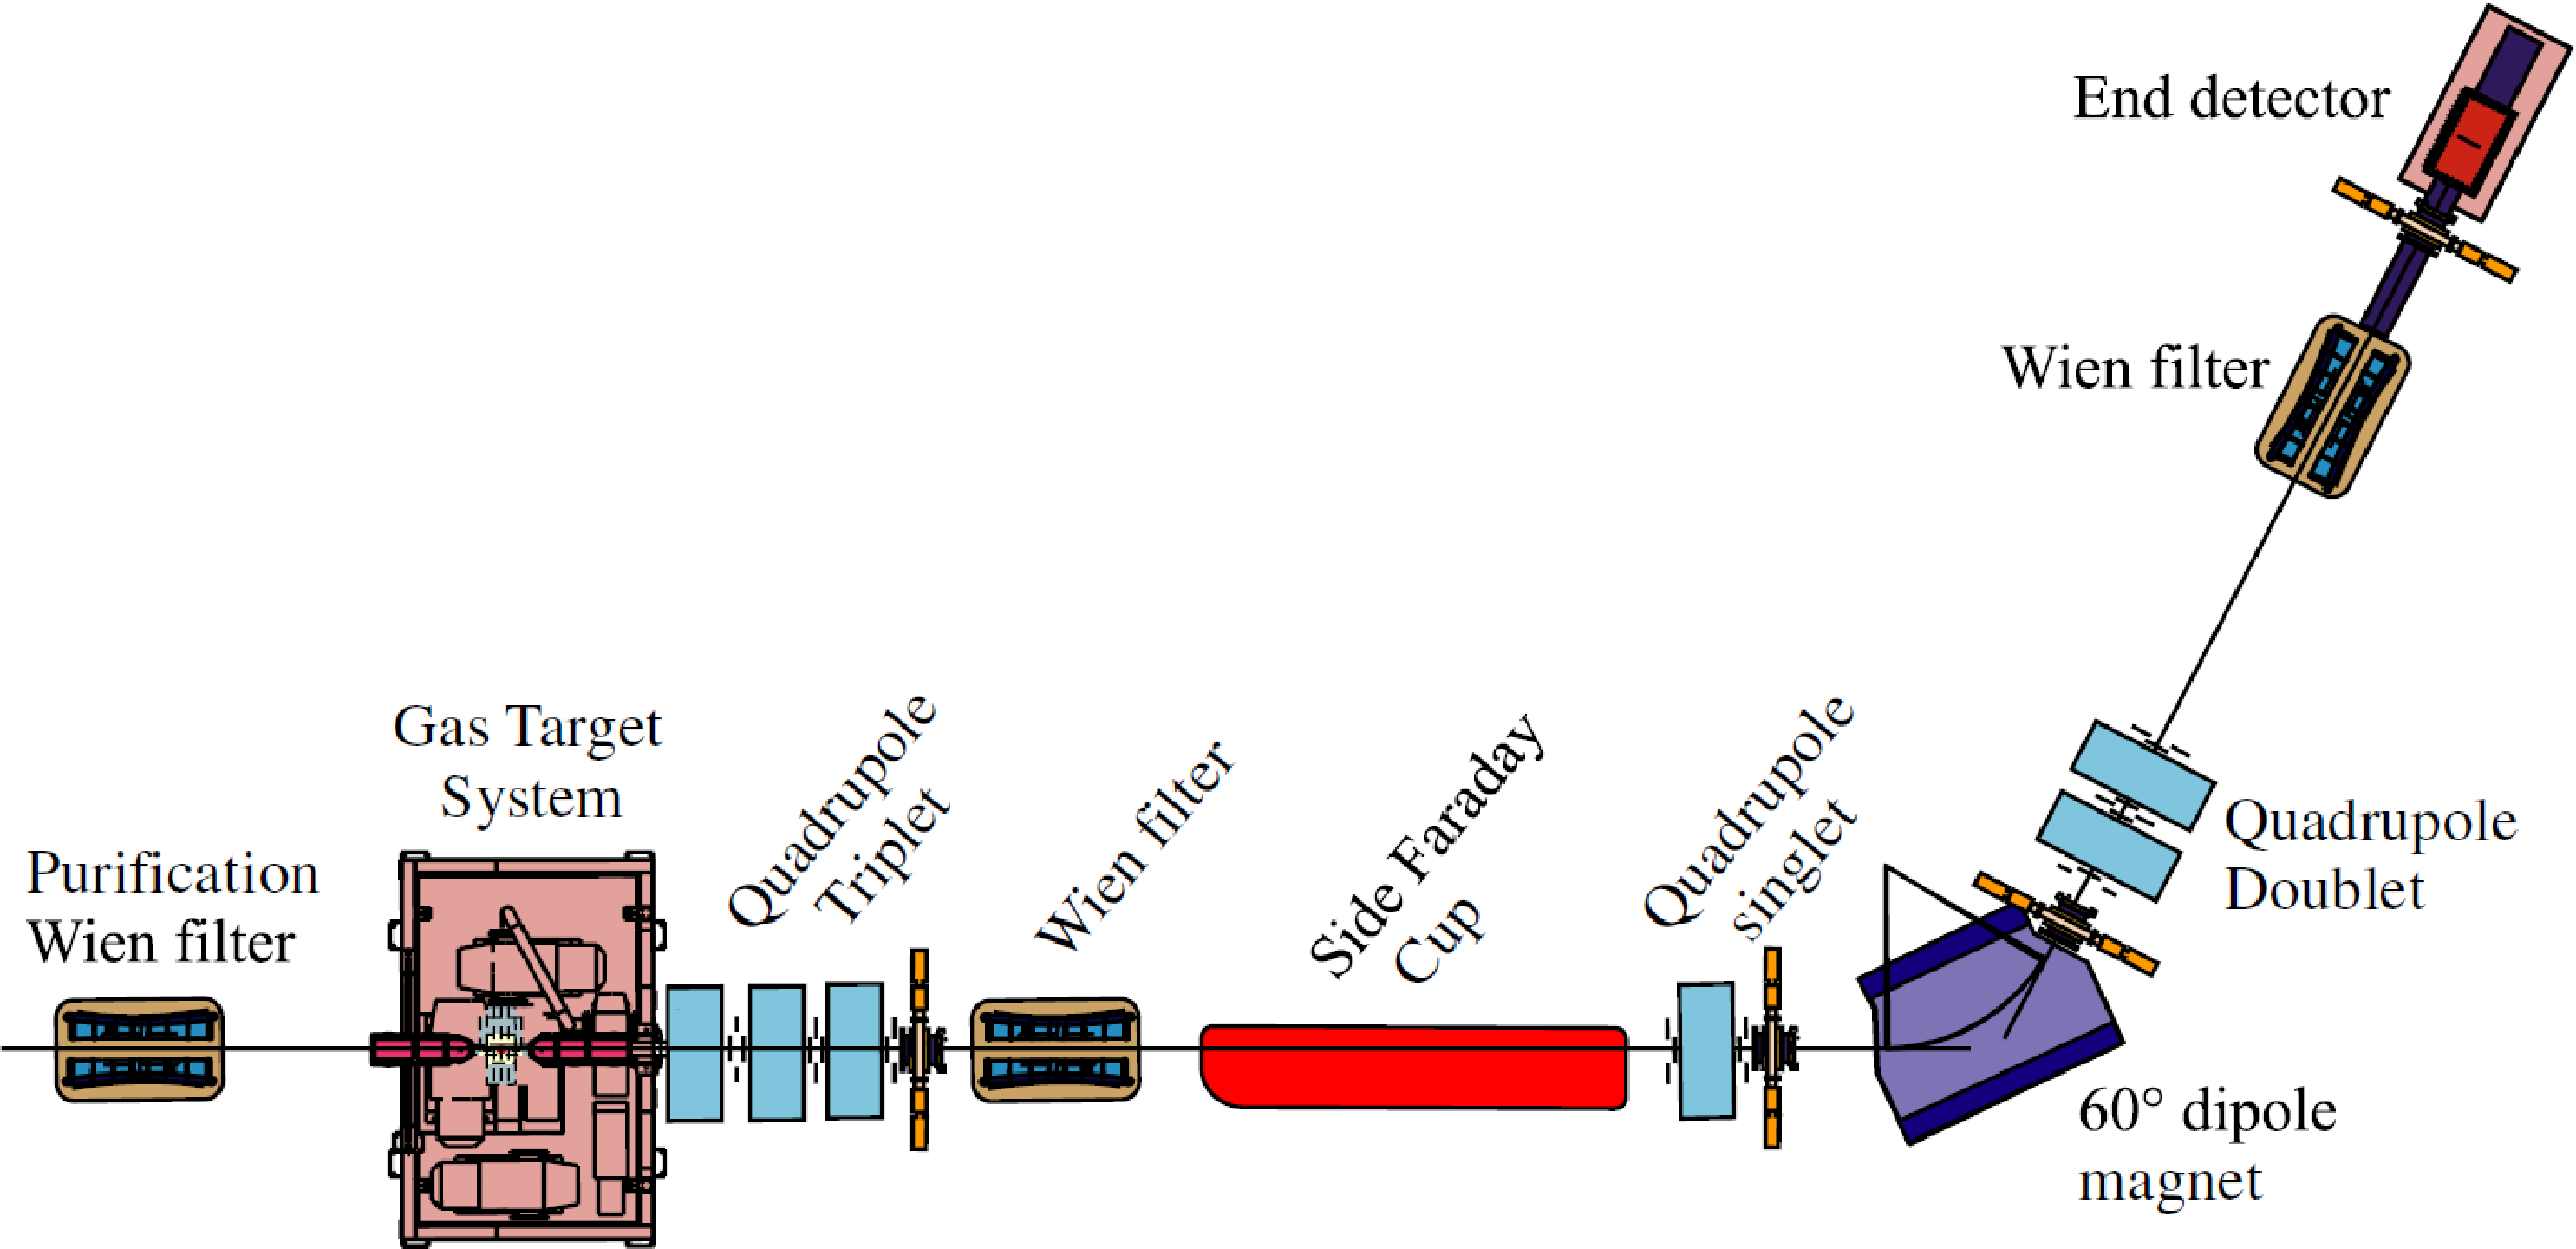
\includegraphics{DiLeva08_Fig2_ERNAschematic}
}
%\vspace{5cm}       % Give the correct figure height in cm
\caption{Schematic view of the ERNA recoil separator. The dispersive elements consist of a Wien filter, a 60-degree magnetic dipole and a second Wien filter.    With electrode voltages up to $\pm$50~kV and lengths of 0.50 and 0.578~m, the Wien filters have a proxy figure of merit 108~kV$\cdot$m.   The design envisaged an energy range of 0.7 to 5~MeV and an angular acceptance 2$\times$31~mrad.Taken from \cite{dile08}.}
\label{fig:erna}       % Give a unique label
\end{center}
\end{figure*}
Figure \ref{fig:erna} shows the eventual setup which in its design was limited by space considerations. For this reason the charge state selection follows the first velocity filter and not vice versa as in the NABONA experiment. The magnetic dipole is then followed by another crossed-field (Wien-) filter device to increase beam suppression. The windowless gas target was constructed to allow placement of $\gamma$ detectors around the gas cell for $\gamma$-recoil coincidence measurements. Recoil detection was initially performed by a segmented ionization chamber but later replaced with a Time-of-flight-Energy (Tof-E) system consisting of a micro-channel plate mirror setup (Tof in conjunction with $\gamma$ detection) and a silicon strip detector. The performance parameters of the system were carefully explored in a series of measurements which are documented in several publications (\cite{roga99,roga03,gial04,schu04,dile08}) over a period of 10 years. ERNA was built for low energy measurements of the \nuc{12}{C}\reac{\alpha}{\gamma}\nuc{16}{O} reaction in inverse kinematics. Among the reactions targeted for proton and alpha radiative capture, this one is unfortunately the most demanding regarding required separator acceptance and beam suppression. The lowest energy in the centre-of-mass system where a measurement with currently available carbon ion beams of ten's of micro-Ampere seems feasible is about \EcmM{0.7}. Here, a separator needs to accept recoils with a half-angle of $\theta_{1/2} = 31 \unit{mrad}$ and $\frac{\Delta{}E}{E} = 12.8\%$. The requirements relax somewhat at higher energies to, {\it e.g.} \EcmM{5}: $\theta_{1/2} = 18 \unit{mrad}$ and $\frac{\Delta{}E}{E} = 7.2\%$. ERNA was nearly able to achieve the low energy benchmark but at the cost of lower beam suppression ranging between $10^{-10}$ and $10^{-12}$ dependent on recoil energies (better at higher energies). An interesting point to note is that the beam suppression deteriorated by a factor of 20 when gas was present in the cell compared to a run without gas. The reason could be additional energy and angle straggling, but most likely is due to the fact that a range of charge states is produced, which in the ERNA design does not filter out in the first selection stage, and which through additional scattering can reach the final focal plane. The tests of the segmented ionization chamber combined with the beam suppression available from the separator revealed that its performance was not sufficient to cover the full targeted energy range for the \nuc{12}{C}\reac{\alpha}{\gamma}\nuc{16}{O} reaction, as the ``leaky'' beam signature encroached on the \nuc{16}{O} recoil signal already at centre-of-mass energies of 2 MeV. An estimate was given that with the available setup measurements down to approximately \EcmM{1.3} would be possible. Improved recoil identification was later provided by adding in the $\gamma$-MCP detector Tof-E condition. As this review focusses on the results of radiative capture measurements using recoil separators with radioactive ion beams, we refer the reader for ERNA scientific results to \cite{schu05,schu05b} (\nuc{12}{C}\reac{\alpha}{\gamma}\nuc{16}{O}) and \cite{dile09} (\nuc{3}{He}\reac{\alpha}{\gamma}\nuc{7}{Be}).
    % Early work at stable beam facilities

\section{Recoil separators at radioactive ion beam facilities}

\subsection{FMA}
The Fragment Mass Analyzer at Argonne National Laboratory~\cite{Da92} was designed for study of high-spin states following heavy-ion fusion.  Like mass separators at Rochester and Legnaro, the FMA has a series of electric, magnetic and electric dipoles.   At $\Delta$V=425~kV and each of length 1.4~m, the two electrostatic dipoles have proxy figure of merit 1260~kV$\cdot$m.  Design acceptances were $\pm$20\% in energy and 8~msr solid angle ($\pm2.3^{\circ}$ in the non-dispersive plane, $\pm2.8^{\circ}$ in the dispersive plane \cite{dav12}), with M/q resolving power of 340.

Although the FMA was not designed to study radiative capture reactions, it was used to successfully study the \pgamma{18}{O}{19}{F} and  \pgamma{18}{F}{19}{Ne} reactions \cite{reh97} (achieving an upper limit on a resonance at \EcmM{0.66}). No further radiative capture reactions have been studied at the facility since this time. It shows however, that recoil separators of this type {\em can} in principle be used for radiative capture, a fact that has implications for future separators of the same EME configuration, such as EMMA at TRIUMF-ISAC. 


\subsection{ARES - Louvain-la-Neuve}

The Astrophysics Recoil Separator (ARES) was the first recoil separator at an ISOL radioactive ion beam facility designed for measurements of \reac{p}{\gamma} reactions in inverse kinematics. It was coupled to the CYCLONE44 cyclotron at the Cyclotron Research Center in Louvain-la-Neuve (Belgium). The cyclotron was dedicated to the acceleration of radioactive ion beams (available in sufficient intensity: \nuc{13}{N} and \nuc{19}{Ne}) in the (0.2 -- 0.8)$\cdot A$ MeV energy range. Compared to electrostatic or linear accelerator facilities CYCLONE44 produces beam with relatively large energy spread ($\frac{\Delta{}E}{E} \approx 1\%$) and emittance ($28\pi \unit{mm\,mrad}$ (horizontal) and $16\pi \unit{mm\,mrad}$ (vertical)), which complicate significantly experiments with recoil separators.
\begin{figure*}
\begin{center}
\resizebox{1.5\columnwidth}{!}{
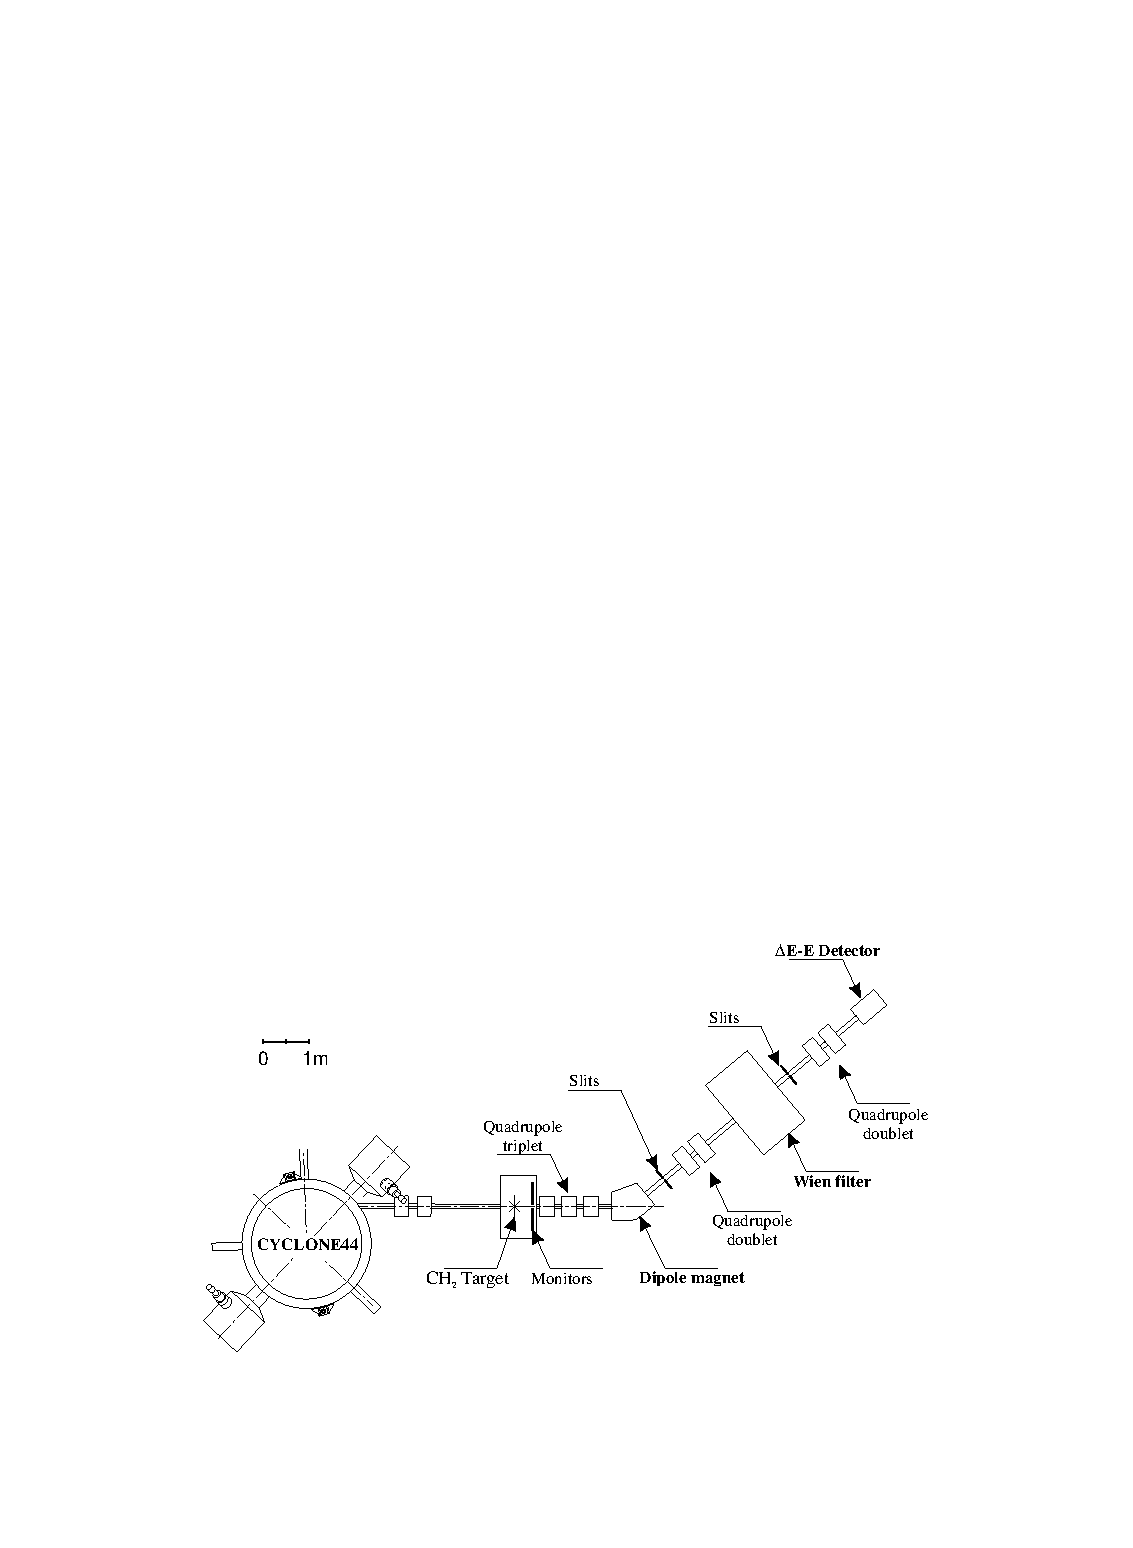
\includegraphics{Couder03_Fig1_ARES}
}
%\vspace{5cm}       % Give the correct figure height in cm
\caption{Schematic view of the ARES separator. Taken from \cite{coud03}.}
\label{fig:ares}
\end{center}
\end{figure*}
Additionally, ARES did not have a gas target available but operated with a plastic foil (CH$_2$) hydrogen target, see Fig. \ref{fig:ares}, thereby reducing resonant yield, and producing additional energy and angle straggling to cope with. The rest of the setup followed the NABONA approach of first using a magnetic dipole to select a charge state to transport and then a crossed field (Wien-) filter to suppress the beam ions of the selected charge state. For recoil detection a $\Delta{}E$-$E$ system combining energy loss measurement in an ionization chamber and residual energy detection in a silicon (PIPS) detector was used \cite{coud03}. Due to the large emittance of the beam direct measurements of the transport efficiency of the separator alone (and thereby deduction of an acceptance) was not possible. Instead, a measurement of the nuclear reaction \nuc{19}{F}\reac{p}{\gamma}\nuc{20}{Ne} was performed in inverse kinematics, and the result compared to simulation and literature data. For this reaction, a selected charge state of the \nuc{20}{Ne} recoils was transported with approximately 11\% transmission efficiency (simulation and experiment in agreement). The rejection factor of the separator proved to be of the order of only $10^{-7}$ resulting from the poor ion beam quality as well as the use of a solid foil target \cite{angu01,coud05}. Nevertheless, the ARES collaboration attempted a measurement of the \nuc{19}{Ne}\reac{p}{\gamma}\nuc{20}{Na} reaction to populate a resonant state at 448 keV having of the order of $10^8 ~\unit{s^{-1}}$ \nuc{19}{Ne} ion beam available. No recoils were detected and an upper limit on the resonance strength of $\omega\gamma = 15.2 \unit{meV}$ established. This limit represents the sensitivity of the separator as defined by the efficiency and primary beam suppression. No further experiments at ARES were performed.

\subsection{DRS - Holifield Radioactive Ion Beam Facility}

The Daresbury Recoil Separator (DRS) was initially designed for use in the UK for the measurement of fusion evaporation reactions in nuclear structure research. With the closure of its accelerator facility, the separator became available for nuclear astrophysics research and was relocated to the newly dedicated Holifield Radioactive Ion Beam Facility (HRIBF) at Oak Ridge National Laboratory (ORNL) \cite{smit98}. It follows in principle the Caltech approach of using a velocity filter (crossed fields) to separate recoils from beam followed by a magnetic dipole ($50^\circ$) to separate charge states. It featured the improvement that two velocity filters were installed in sequence with an additional focus and selection slits in between them, as shown in Fig.\ \ref{fig:drs}.
\begin{figure*}
\begin{center}
\resizebox{1.5\columnwidth}{!}{
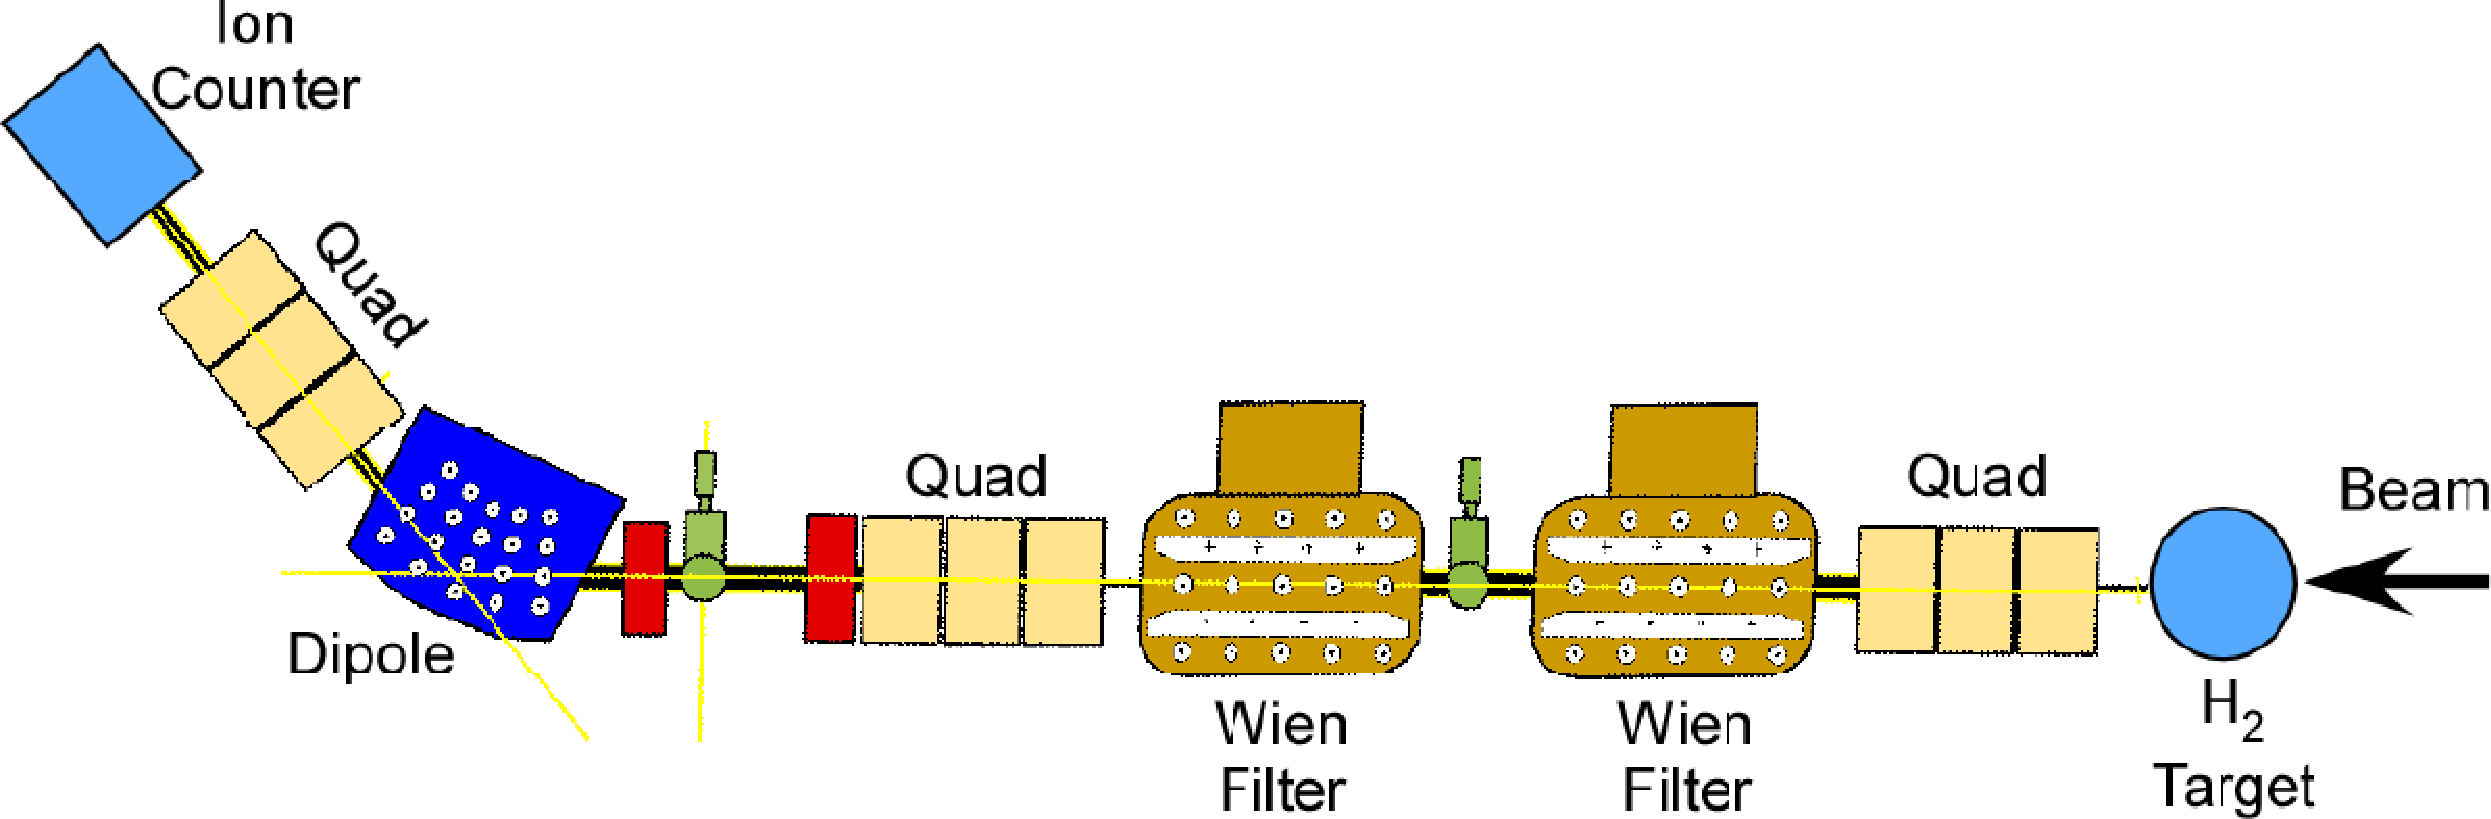
\includegraphics{Bardayan09_Fig1_DRS}
}
%\vspace{5cm}       % Give the correct figure height in cm
\caption{Schematic view of the DRS separator. Dispersive elements are a pair of Wien filters followed by a 50-degree magnetic dipole.   With maximum design voltage $\Delta$V=600~kV and each of length 1.28~m, the two Wien filters have a proxy figure of merit 1536~kV$\cdot$m.
Design acceptances were 2$\times$45~mrad in horizontal and vertical angles, $\pm$2\% in velocity and  $\pm$1.2\% in M/q, with resolving power 300 in M/q.Taken from \cite{bard09}.}
\label{fig:drs}
\end{center}
\end{figure*}
The HRIBF uses a light ion cyclotron to drive an on-line radioactive ion source which injects negative ions into the vertical folded tandem accelerator with a maximum terminal voltage of 25 MV. For nuclear astrophysics research the facility focused on the production of radioactive fluorine isotopes relevant to the hot and explosive CNO cycles. Measurement of radiative capture in this mass regime however required running the Tandem close to the lower voltage limits sacrificing transmission efficiency. For these measurements the DRS was coupled with a windowless Hydrogen gas target capable of maintaining 5.5 Torr pressure over 15 cm target length. The acceptance of the separator was only limited in these experiments by the diameter of the gas flow limiting apertures. These were tailored to accept the specific reaction recoils pursued. In the final focal plane of the separator a $\Delta{}E-E$ ionization chamber (IC) provided nuclear charge (Z) identification. Additionally, a position sensitive MCP detector was available to position in front of the IC to map the recoil hit positions. Ion beam suppression factors of order $10^9 - 10^{11}$ were achieved, varying with beam energies and conditions. The DRS was tested with proton capture on stable \nuc{24}{Mg}, \nuc{17}{O} and \nuc{12}{C} and used for measurement of the radioactive beam reactions \nuc{1}{H}(\nuc{17}{F},$\gamma$)\nuc{18}{Ne} and \nuc{1}{H}(\nuc{7}{Be},$\gamma$)\nuc{8}{B}. 


\subsection{DRAGON - TRIUMF-ISAC}
The DRAGON Facility (Detector of Recoils And Gammas Of Nuclear reactions) was designed to provide a recoil separator to study radiative capture reactions, both on protons and alpha particles, using post-accelerated radioactive ion beams at the ISAC facility \cite{hut03a,hut03,eng05}. The ISAC facility \cite{ball11} provides ISOL beams using a 75$\mu$A, 500 MeV proton beam from the TRIUMF sector-focusing cyclotron. These are reaccelerated through a 35 MHz radio-frequency quadrupole with $A/q\leq30$, and a 105 MHz variable energy drift-tube-linac with $3\leq A/q\leq6$, between energies of 0.15$A$ MeV and 1.5$A$ MeV \cite{lax02}.  This energy regime, particularly the lower end, is well-suited to performing radiative capture reactions of the type occurring in classical novae and type 1 X-ray bursts, and given the high beam quality (typical beam emittance is on the order of  $\beta\epsilon_{x,y}=0.2\pi$ mm$\cdot$mrad, $\epsilon_{l}=1.6A$ keV$\cdot$ns) and beam intensity (e.g. $^{21}$Na=$1\times10^{9}$ s$^{-1}$, $^{26g}$Al=$1\times10^{10}$ s$^{-1}$) achievable, a wide range of proton- and alpha- radiative captures become available for measurement. 

Construction started on DRAGON in 1999 and commissioning was performed during the 2001-2003 period using $^{21}$Na radioactive beams over the entire ISAC energy range to study $^{21}$Na($p,\gamma$)$^{22}$Mg in detail \cite{dau04}. The facility is based around a recirculating, windowless extended gas target, capable of holding up to $\approx 7.6$ Torr of H$_{2}$ or He gas over an effective length of 12.3 cm, leading to target thicknesses of up to $6 \times 10^{18}$ cm$^{-2}$ (for hydrogen at 300 K). The target gas is recirculated using a set of inline high-compression Roots blowers through a liquid-nitrogen cooled zeolite matrix to trap impurities, while the beamline on either side of the target is differentially pumped in a series of tubes leading to pressures of ~$1\times 10^{-6}$ Torr at the entrance to the ion-optical part of the separator. The gas cell (see figure \ref{fig:dra_gas_target}) is composed of a trapezoidal volume with thin aluminium walls to mitigate photon absorption, with a 6 mm aperture at the upstream side and an 8 mm aperture at the downstream side. The trapezoidal shape ensures that the hydrogen flow is angled down towards the root blowers and thus discourages supersonic flow into the beam-pipes. 

\begin{figure}
\resizebox{1.1\columnwidth}{!}{
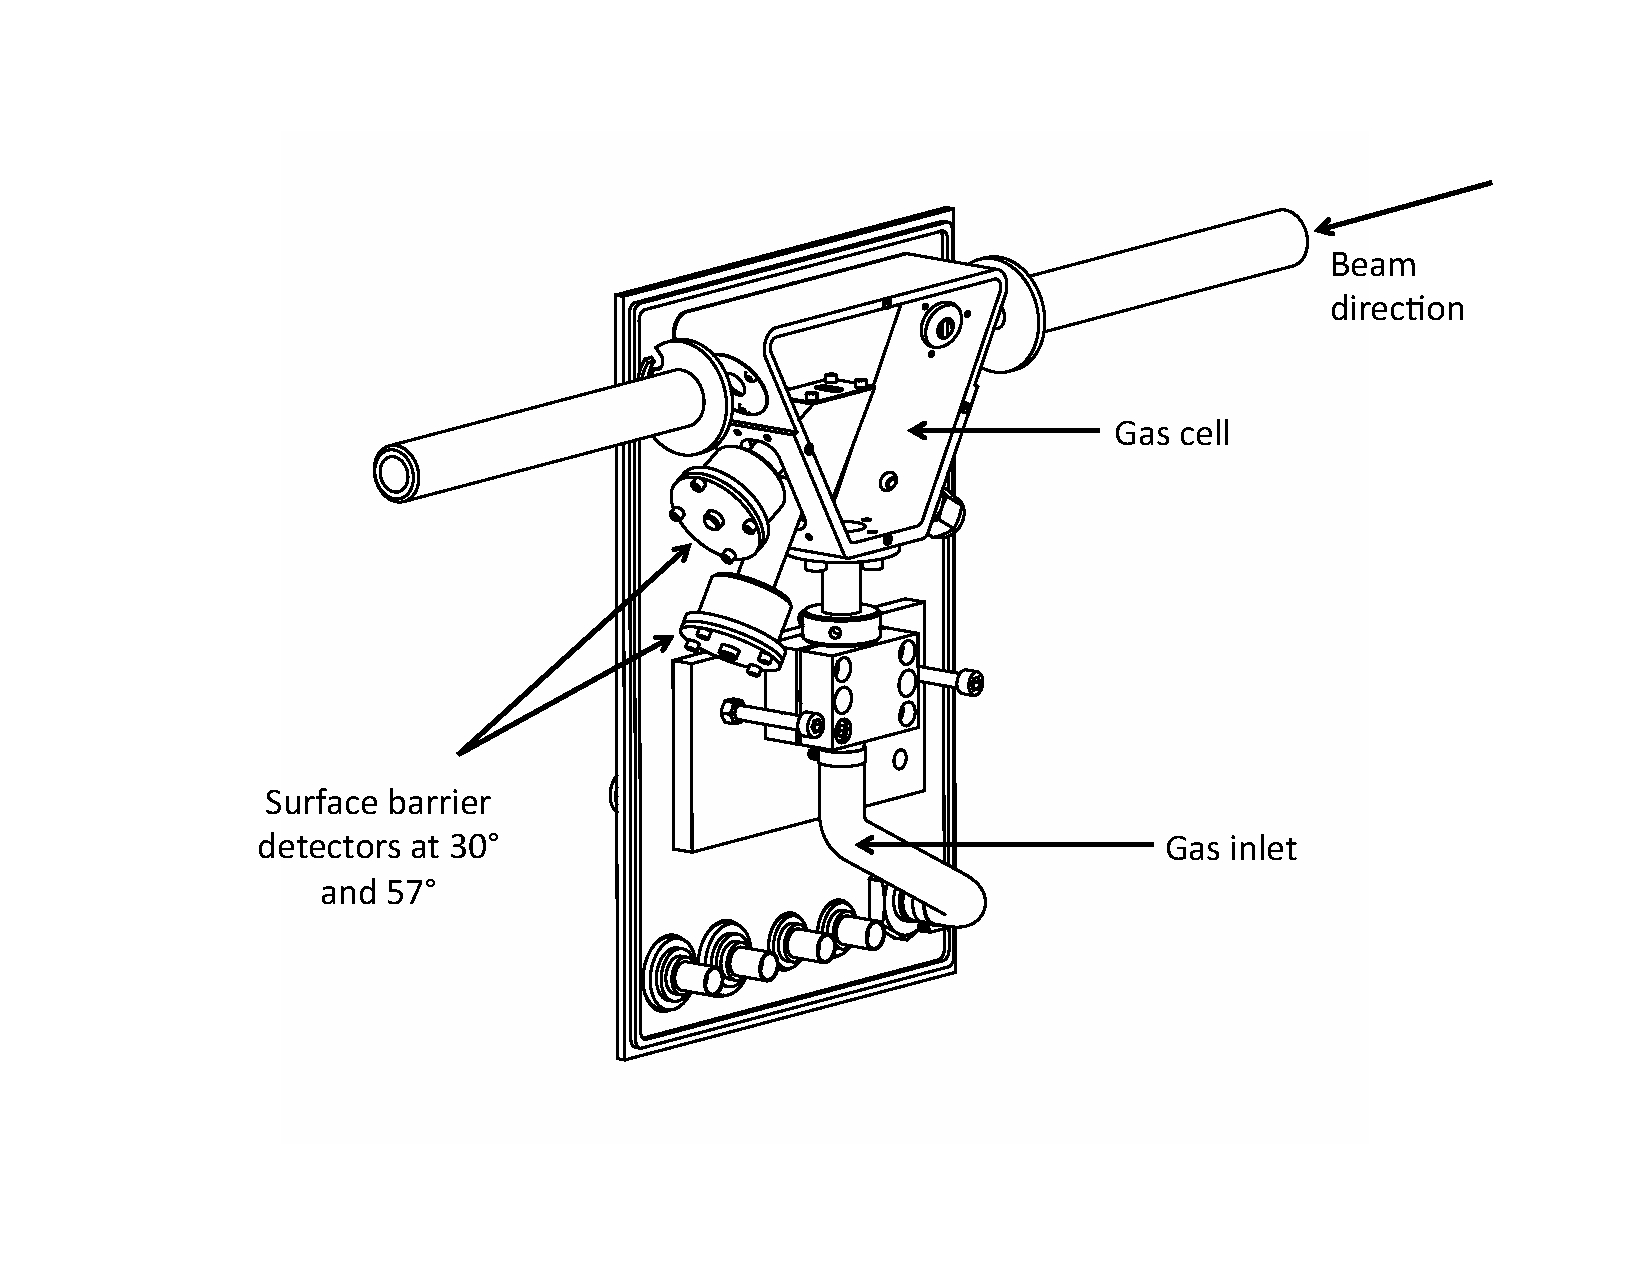
\includegraphics{dra_gas_target}
}
%\vspace{5cm}       % Give the correct figure height in cm
\caption{The DRAGON windowless gas target, showing the trapezoidal gas volume and gas inlet, surface barrier detectors and inner pumping tubes.  }
\label{fig:dra_gas_target}
\end{figure}

The ion optical configuration of DRAGON is a {\bf MEME} design, consisting of magnetic and electric  dipole elements of bending angles $\phi=$50$^{\circ}$,20$^{\circ}$,75$^{\circ}$ and 35$^{\circ}$, and bending radii $\rho$=100 cm, 200 cm, 81.3 cm and 250 cm respectively (figure \ref{fig:dra_optics}). The particular configuration was designed specifically around the recoil distribution expected from the $^{15}$O($\alpha ,\gamma$)$^{19}$Ne reaction at $E_{c.m.}=0.51$ MeV. It was thus designed with a geometric acceptance of $\pm21$ mrad at the central energy, and an energy acceptance of $\pm4\%$ at the central trajectory. 
\begin{figure*}
\begin{center}
\resizebox{1.6\columnwidth}{!}{
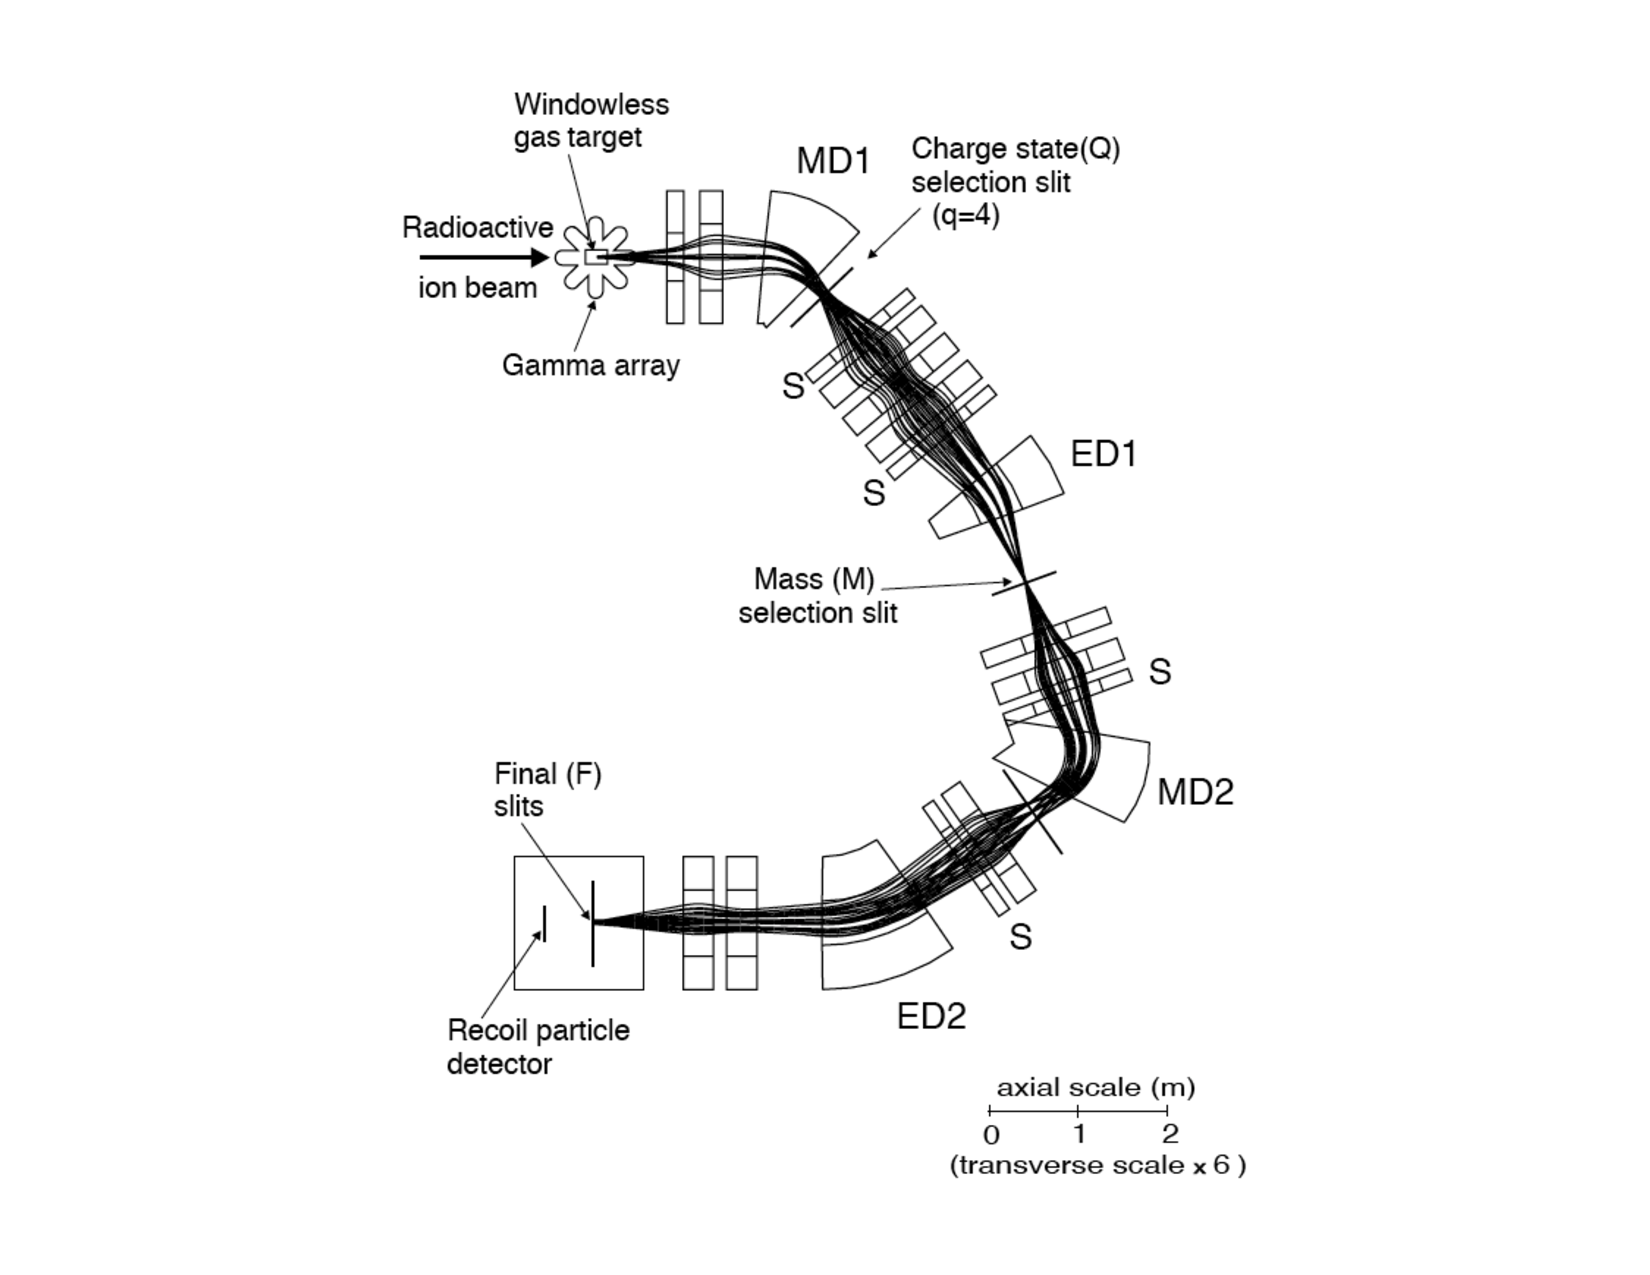
\includegraphics{dra_optics}
}
%\vspace{5cm}       % Give the correct figure height in cm
\caption{Schematic representation of the DRAGON recoil separator (taken from \cite{hut03}). The electrostatic dipoles, with respective lengths 0.7 and 1.57~m and voltages $\pm$200 and $\pm$160~kV, give a proxy figure of merit 780~kV$\cdot$m.  Design angular acceptance was 2$\times$21~mrad with beam energies in the range 0.15 to 1.5~MeV per nucleon. The transverse scale has been magnified 6X to display apertures and trajectories.}
\label{fig:dra_optics}
\end{center}
\end{figure*}

The first magnetic dipole (MD1) of the separator is used to select a single charge state for beam and recoils, using a set of slits located at the first energy-dispersed focus after MD1. This focus has an energy dispersion of 0.3 cm/\% and a magnification of -0.44 in the horizontal direction. The energy of the beam/recoils in their chosen charge state can thus be measured by centring on the slits at this focus and relating the magnetic field -- measured using an NMR probe positioned in the central flat field region of the dipole -- to the beam energy via the magnet calibration constant, which has been determined using several well-known stable beam proton capture resonances. Thus a direct measurement of the beam energy with and without gas in the target allows a determination of the target energy loss, which when combined with the effective length, gives the stopping power. 

The first mass-separation stage stage of the DRAGON separator occurs after the first electric dipole element, at a set of slits at the mass-dispersed achromatic focus. The second stage of the separator is essentially a copy of the first. The overall mass resolution at the final focus of the separator is around 0.3\% for a typical object size at the gas target central position.  

%Acceptance, suppression, rigidity, background rejection, resonance energy determination (both BGOs)
The overarching quality of DRAGON is the separator beam suppression. As can be seen in ref. \cite{hutc08}, the raw beam suppression of the separator (for proton capture)\footnote{In general, for alpha-capture reactions on a given beam mass, better beam suppression is achieved. This can be compounded further in a few light-mass cases where the availability of beam charge-states is reduced, as can be seen in the extreme case of $^{3}$He($\alpha$,$\gamma$)$^{7}$Be, where a $^{7}$Be charge state can be selected for which there is no similar beam A/Q, leading to extremely high separator suppression values (see ref. \cite{sju12}).} is on the order of 10$^{8}$-10$^{13}$, depending on the incident beam energy. This is directly correlated to the emittance of the delivered beam, which results in a larger and more divergent beam at the target position for lower energies, and thus aperture scattering in the target and pumping tube region, and elsewhere in the separator, can result in orders of magnitude difference in the fraction of incident beam particles that reach the final focus. As it stands, this is well suited to the range of radiative capture reactions to be studied, with reaction yields on the order of down to 10$^{-14}$ reaction per incident beam particle. This means that for weak reactions, the 'leaky beam' rate at the focal plane detectors can be a couple to a few orders of magnitude lower or higher than the expected reaction signal. Local time of flight and particle energy or stopping power measurement can then be used to identify the particles, leading to higher effective orders of background suppression. In DRAGON's case a 5 cm $\times$ 5 cm, 256-quasi-pixel double-sided silicon strip detector can be used, or a 4-anode isobutane-filled ionization chamber, for final particle detection, the latter offering an additional degree of atomic-number discrimination through differential energy loss of the ions through the anode regions. These detectors are located approximately 60 cm from DRAGON's focal plane.

On either side of the focal plane, separated by 59 cm are two microchannel plates offering a minimally-destructive local time-of-flight system capable of ~400 ps resolution, sufficient to provide excellent mass separation between the reaction products and leaky beam particles. Ref. \cite{vock09} provides a detailed description of this device, which relies on thin diamond-like-carbon (DLC) foils and electroformed meshes to function according to requirements. 

The DRAGON separator is designed for beam rigidities of up to 0.55 T$\cdot$m. The limiting factors are (a) the maximum achievable magnetic field strength at the first magnetic dipole and (b) the maximum sustainable voltage between the electrodes of the first electric dipole. The magnetic field limit is the limiting factor below ion energies of $1.34A$ MeV, for a maximum field of 0.55 T, while the electric field is the limit above this energy, corresponding to a maximum setpoint voltage of 230 kV (corresponding to a field strength of 4.6 MV/m). Figure \ref{fig:rigidity} shows the limiting curves for maximum bendable ion energy versus ion mass-to-charge ratio.   

\begin{figure}\resizebox{1.0\columnwidth}{!}{
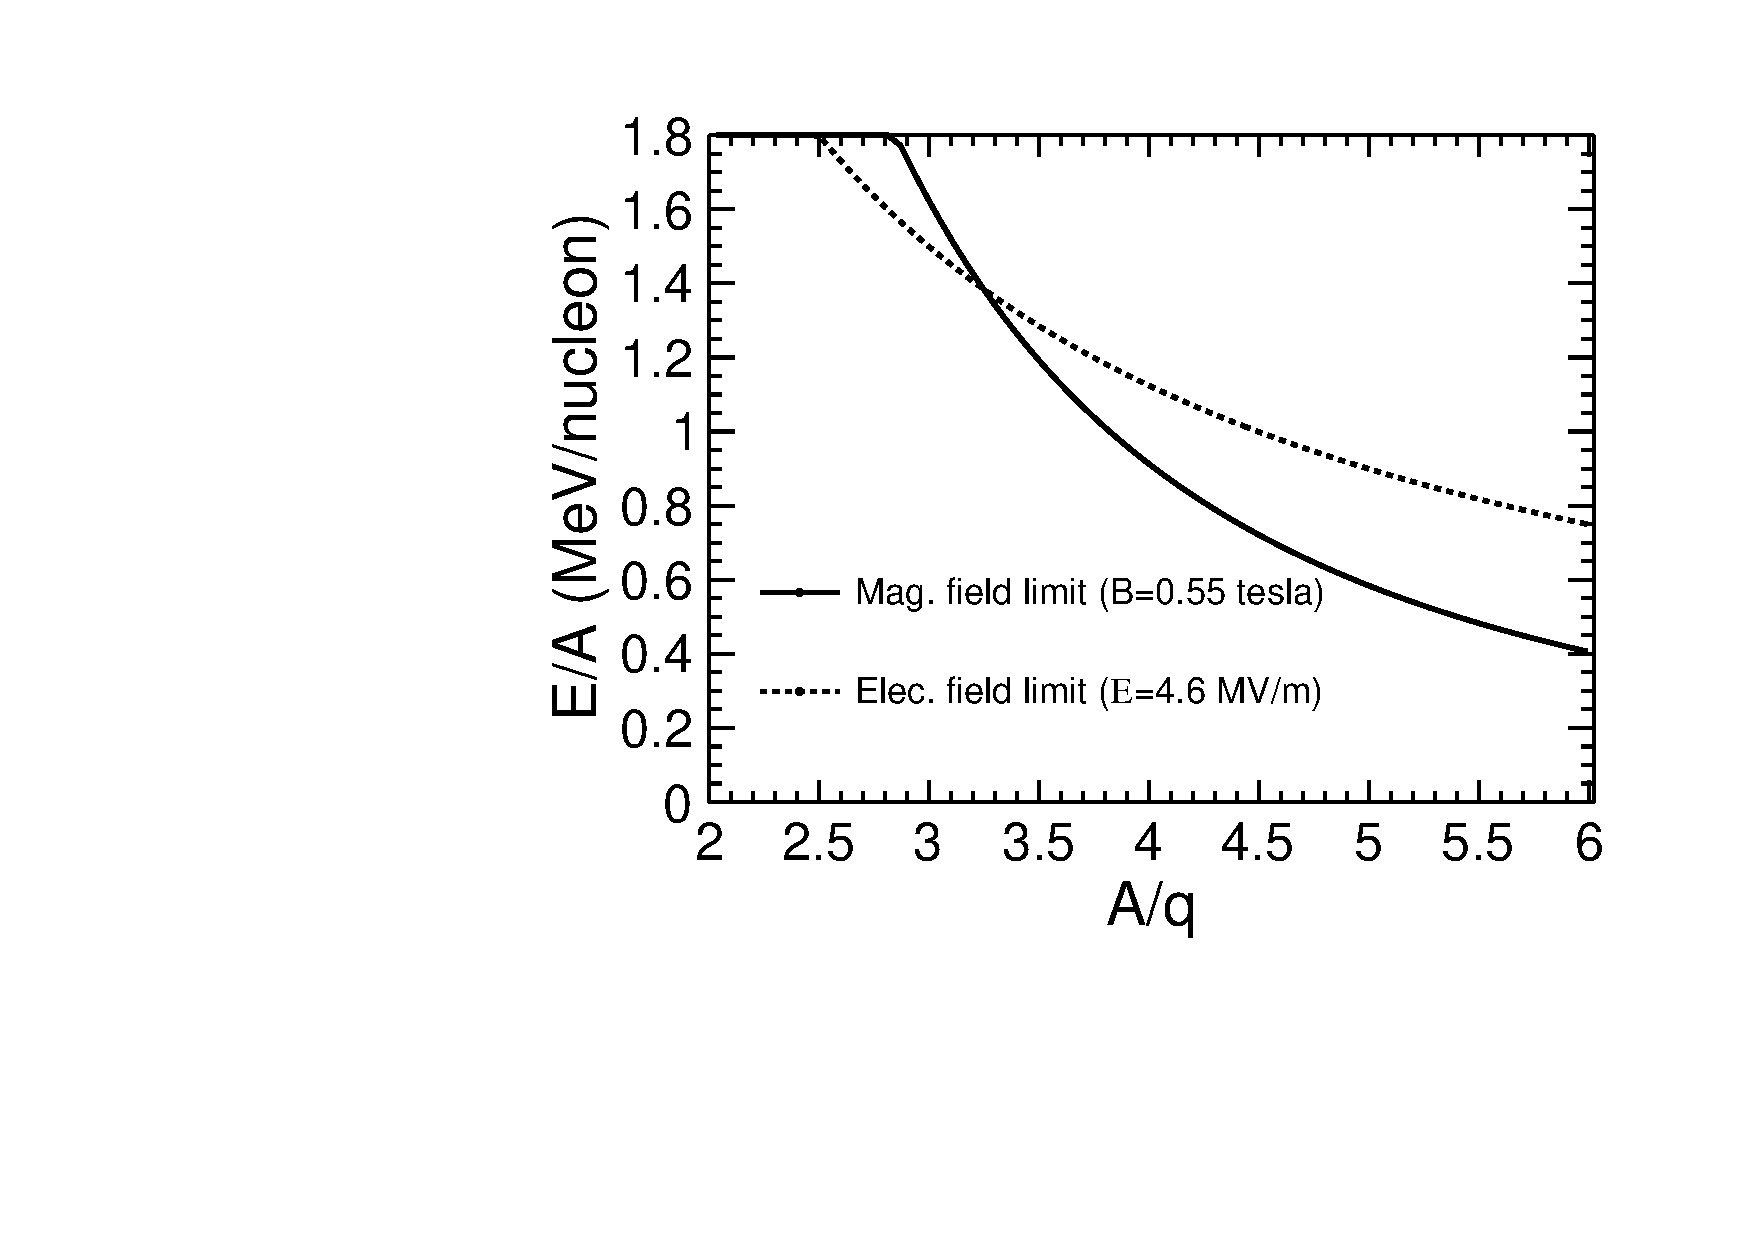
\includegraphics{rigidity}
}
%\vspace{5cm}       % Give the correct figure height in cm
\caption{Magnetic and electric limits for the DRAGON separator, showing the maximum ion energy that can be bent around the magnetic and electric dipoles for a given mass-to-charge ratio. Above $1.38A$ MeV, the limit is the sustainable field on the electric dipole. Below this, the power supply and cooling on the magnetic dipole is the hardware limit.}
\label{fig:rigidity}
\end{figure}

To provide additional background rejection to the focal plane detectors, recoil ions are tagged with prompt $\gamma$-rays emitted from the reaction at the gas target. These are detected using a 30-element bismuth germanate (BGO) array consisting of hexagonal crystals roughly 6~cm in diameter and 8~cm deep arranged so as to give nearly 4$\pi$ solid angle coverage \cite{gig03}. BGO was chosen primarily because of its high efficiency (high absorption for $\gamma$-rays due to the high material density and a large scintillation light output), but also because of its relatively inexpensive nature compared to faster or brighter scintillators such as lanthanum bromide (LaBr$_{3}$) or lutetium oxyorthosilicate (LSO). Because the recoil ions are the primary detection object, high energy resolution is not really necessary, the 10\% or so given by BGO being sufficient for most purposes. The segmentation of the array also allows individual cascade $\gamma$ rays to be detected, giving an overall very high efficiency in the range 40-80\% dependent on the energies and quantity of $\gamma$ rays\footnote{In a given cascade of $N$ $\gamma$ rays, the probability of detecting at least one of them is given by $P=1-\Pi^{N}_{i=1}(1-\epsilon_{i})$ where $\epsilon_i$ here represents the efficiency of detecting the $i$th $\gamma$ ray and encompasses all geometric and energy-dependent factors. With typical values of $\epsilon$ around the 40\% mark for the almost $4\pi$ coverage DRAGON BGO array, it is easy to see how cascades of 3 $\gamma$ rays for example, can lead to high detection efficiency.}. 

By detecting prompt $\gamma$ rays, and by determining the time-of-flight between them and the recoil ion detection, 2-3 orders of magnitude further effective beam suppression (random background rejection) can be achieved on top of the raw separator suppression and particle identification. The BGO efficiency (see ref. \cite{gig03} for details on how it is measured) however, is the major systematic error in such a measurement, and it dominates the total systematic error of the experiment.  

The BGO array, because of its segmentation along the beam (z) axis, can also provide information on the location of the reaction origin for a narrow resonance via the BGO hit pattern. This, coupled with the beam-in-gas stopping power (derived by measuring the beam energy at the energy-dispersed focus with and without gas in the target) allows a determination of the resonance energy, to a precision of 0.5\% \cite{hut12}.
 
The DRAGON facility started its experimental program by extensively studying the radioactive beam reaction $^{21}$Na($p,\gamma$)$^{22}$Mg during 2000-2003 \cite{dau04}, following over the years with the other RIB studies  $^{26g}$Al($p,\gamma$)$^{27}$Si \cite{rui06}, $^{23}$Mg($p,\gamma$)$^{24}$Al \cite{eri10} and $^{18}$F($p,\gamma$)$^{19}$Ne \cite{ake13} (some of these are discussed in more detail in the following sections). At the time of writing of this article DRAGON had recently performed measurements of $^{26m}$Al($p,\gamma$)$^{27}$Si. In addition studies have been performed for the stable beam alpha-capture reactions $^{12}$C($\alpha$,$\gamma$)$^{16}$O \cite{mat06}, $^{40}$Ca($\alpha$,$\gamma$)$^{44}$Ti \cite{voc07,voc08}, $^{17}$O($\alpha$,$\gamma$)$^{21}$Ne, $^{16}$O($\alpha$,$\gamma$)$^{20}$Ne \cite{hag12b} and $^{3}$He($\alpha$,$\gamma$)$^{7}$Be \cite{sin12}, and for the proton-capture reactions ~~~$^{17}$O($p,\gamma$)$^{18}$F \cite{hag12} and $^{33}$S($p,\gamma$)$^{34}$Cl \cite{fal13}. In addition, a high mass capture reaction study was performed at DRAGON to demonstrate its ability to perform as a recoil separator far beyond its design limit. The reaction chosen was $^{58}$Ni($p,\gamma$)$^{59}$Cr \cite{Sim13}, and the success of this study prompted the consideration of more alpha capture reactions above the $A=76$ region for the p-process.  Forays into this region began at DRAGON in earnest with the measurement of $^{76}$Se($\alpha$,$\gamma$)$^{80}$Kr \cite{Fal14}. 




 
               % Recoil separators at radioactive ion beam facilities

\section{Scientific highlights}

\subsection{\nuc{7}{Be}\reac{p}{\gamma}\nuc{8}{B} (NABONA and DRS) }
The proton radiative capture on \nuc{7}{Be} ($T_{1/2} = 53.3$ days) is one of the most important reactions in nuclear astrophysics as it determines the number of the highest energy neutrinos emerging from a hydrogen burning star like our sun. As human science has now entered the precision phase in solar neutrino detection with real time detectors like SNO, Super-Kamiokande and Borexino, the error on the rates of the neutrino producing nuclear reaction in the hydrogen burning chains become the limiting factors in the interpretation of the measured neutrino fluxes. Our cross section information so far encompasses predominantly solid \nuc{7}{Be} targets of varying purity, complemented with data from Coulomb breakup experiments where the inverse reaction is measured. With claimed uncertainties below 5\% the measurements fall within a 20\% band suggesting that systematical uncertainties are present. In order to try an approach with different systematic uncertainties two attempts were made so far to measure this reaction using a radioactive beam and recoil separator detection. In both cases the radioactive material was not produced on-line but sent from an off-site producer, chemically treated and concentrated before being used in a standard sputter source \cite{gial00}. The first attempt at this reaction was performed with the NABONA recoil separator in Naples. The accelerator provided an 8 MeV \nuc{7}{Be} ion beam in the $4^+$ charge state of up to 30 epA varying over several days. This intensity was unfortunately not sufficient to make a statistically significant measurement yielding only 13 recoil events identified as \nuc{8}{B} by the $\Delta{}E-E$ IC in the focal plane (Fig.\ \ref{fig:gialanella00_fig2}: Fig. 2 from \cite{gial00}).
\begin{figure}
\begin{center}
\resizebox{0.95\columnwidth}{!}{
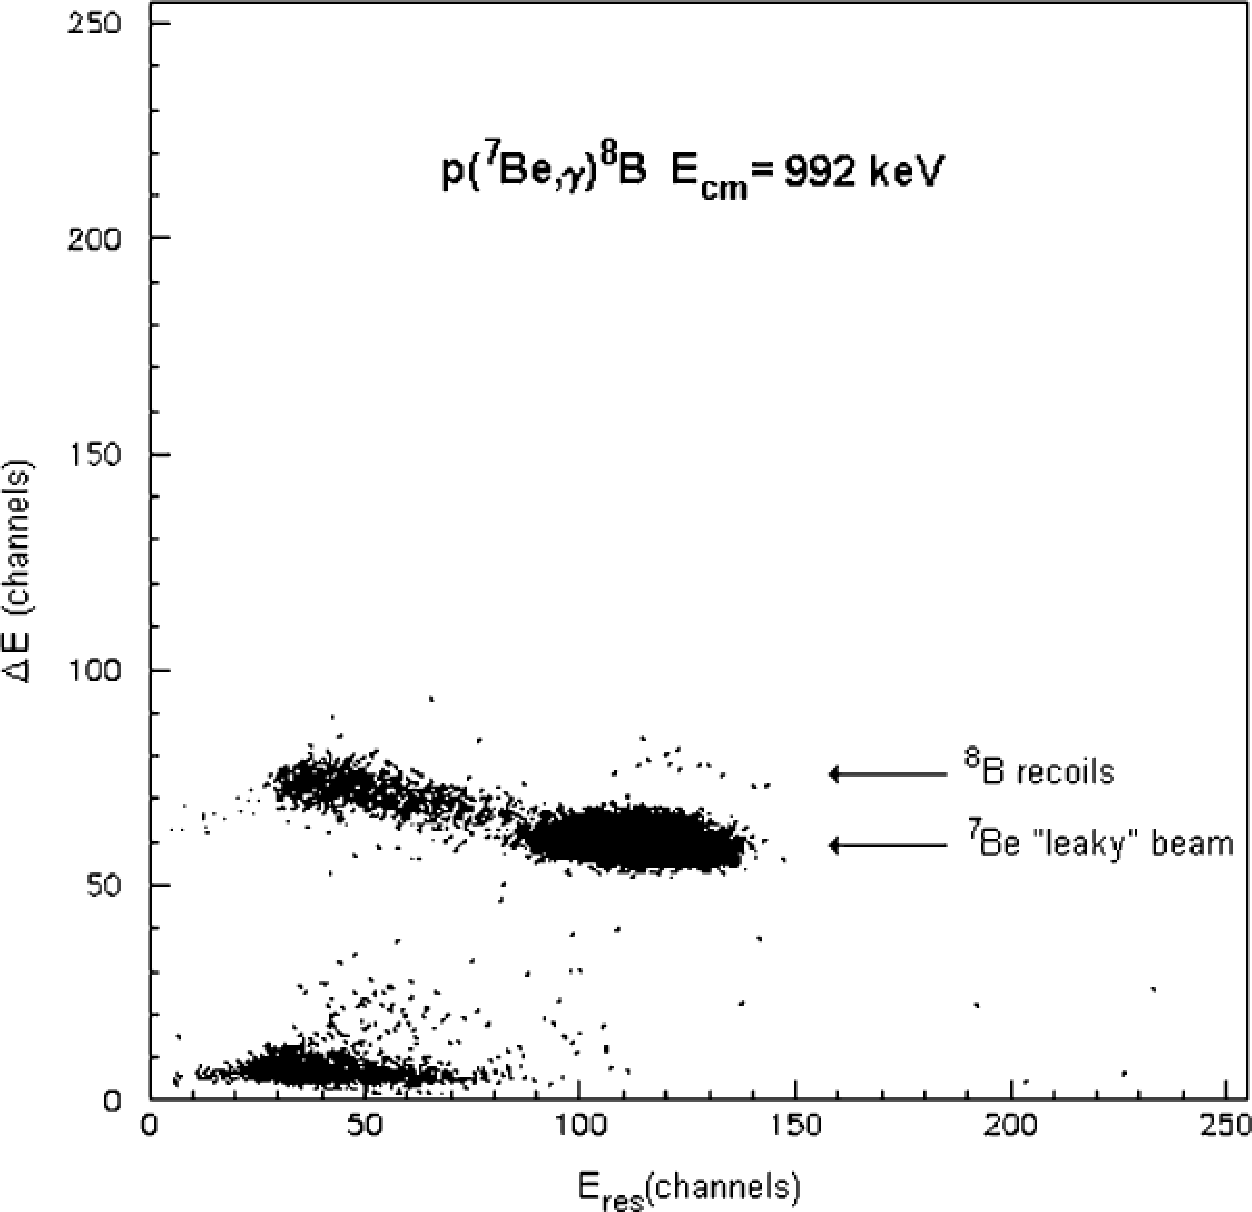
\includegraphics{Gialanella00_Fig2_DeltaE-E}
}
\caption{Two dimensional density plot of the $\Delta{}E-E$ telescope with the recoil separator tuned to the \nuc{8}{B}$^{5+}$ nuclides from $p$(\nuc{7}{Be},$\gamma$)\nuc{8}{B} reaction. The observed structures are identified. Taken from \cite{gial00}.}
\label{fig:gialanella00_fig2}
\end{center}
\end{figure}
The beam intensity produced in Naples already required performance of the radiochemical procedures with activities of the order of 10 -- 20 GBq and it was not deemed practical to increase on these. Therefore, this reaction was not pursued further at this accelerator facility. Several years later, the HRIBF facility was able to increase ion source efficiency and accelerator transmission but was only capable to handle a reduced activity in the radiochemistry. Therefore, they achieved a similar \nuc{7}{Be} ion beam intensity, this time stable over several days, but again only an insufficient number of recoils (Fig.\ \ref{fig:bardayan09_fig4}: Fig. 4 of \cite{bard09}).
\begin{figure}
\begin{center}
\resizebox{0.98\columnwidth}{!}{
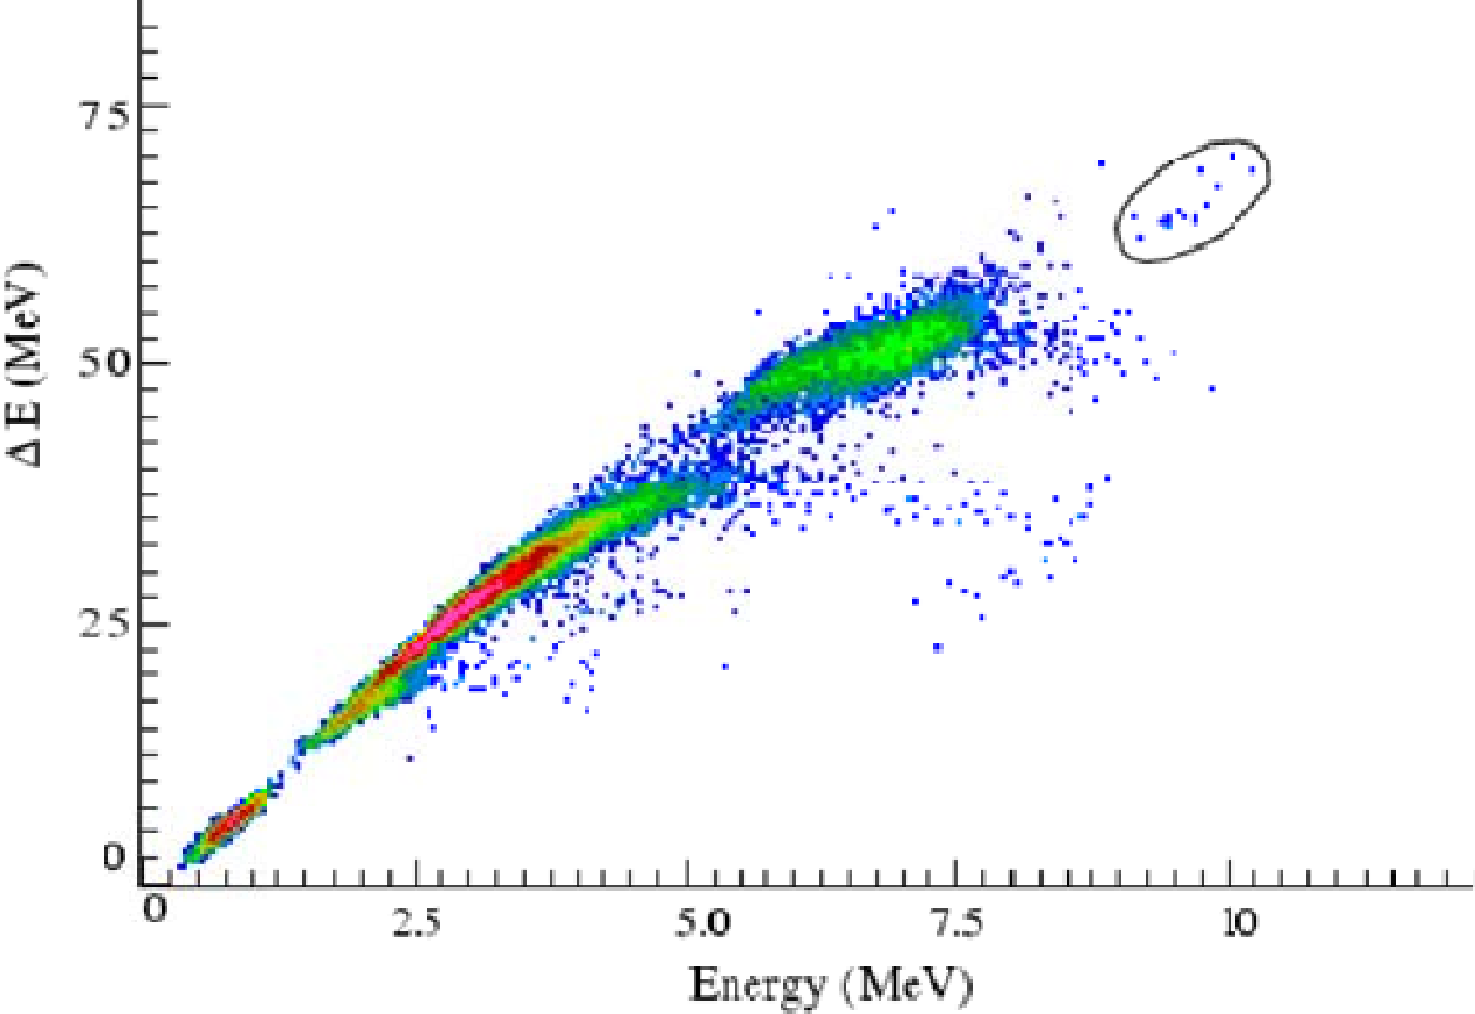
\includegraphics{Bardayan09_Fig4_Be7pg_DeltaE-E.pdf}
}
\caption{An ion counter $\Delta{}E$ vs. $E$ spectrum obtained for the \nuc{1}{H}(\nuc{7}{Be},$\gamma$)\nuc{8}{B} reaction. Events from \nuc{8}{B} recoils are circled. Taken from \cite{bard09}.}
\label{fig:bardayan09_fig4}
\end{center}
\end{figure}%
Significant to mention is that both attempts did not need $\gamma$ detection but it was sufficient to use nuclear charge identification with an IC at the focal plane. Although both experiments were performed at the same beam energy with similar gas target configurations, the leaky $^7$Be beam signature in the equally similar focal plane detectors appears very different probably due to the differences in separator configuration. It should be noted that in both attempts methods were developed to achieve the required uncertainties in {\it e.g.} beam normalization and solid angle determination. However, as it became clear that the statistics to return a relevant data point could not reached, many of these ancillary measurements were not followed through on. 


\subsection{\nuc{21}{Na}\reac{p}{\gamma}\nuc{22}{Mg} (DRAGON)}
The \nuc{21}{Na}\reac{p}{\gamma}\nuc{22}{Mg} reaction was the first to be measured with radioactive beam at the DRAGON facility, and the high intensity $^{21}$Na beam was one of the first to be accelerated at TRIUMF-ISAC, being a relatively easy ISOL beam to produce because of the high surface ionization efficiency of sodium using high-power silicon-carbide targets at ISAC, which are capable of producing pure $^{21}$Na beams on the order of $1 \times 10^{10}$ s$^{-1}$. 
The \nuc{21}{Na}\reac{p}{\gamma}\nuc{22}{Mg} reaction itself is a potential bypass to the $\beta^{+}$ decay of $^{21}$Na in the Ne-Na-Mg cycle that occurs in O-Ne-Mg novae. When \nuc{21}{Na}\reac{p}{\gamma}\nuc{22}{Mg} becomes faster than the decay, $^{22}$Na is made sooner. If this happens at times when the expanding nova envelope is hotter, $^{22}$Na can then be destroyed more quickly via proton capture. The net effect is that the faster \nuc{21}{Na}\reac{p}{\gamma}\nuc{22}{Mg} is at peak nova temperatures, the less $^{22}$Na survives in the ejecta. Since $^{22}$Na is one of the most promising candidates for direct observation from novae, it is important that the \nuc{21}{Na}\reac{p}{\gamma}\nuc{22}{Mg} reaction is known to sufficient precision to remove the nuclear physics uncertainty from $^{22}$Na ejected yield predictions.  

The \nuc{21}{Na}\reac{p}{\gamma}\nuc{22}{Mg} reaction at nova temperatures is dominated by several strong resonances corresponding to states in $^{22}$Mg. These states were identified previous to the DRAGON experiment in several indirect studies such as $^{24}$Mg(p,t)$^{22}$Mg \cite{bat01,mic02} and $^{25}$Mg($^{3}$He,$^{6}$He)$^{22}$Mg \cite{cag02}, as well as $^{12}$C($^{16}$O,$^{6}$He)$^{22}$Mg \cite{che01}, and $^{20}$Ne($^{3}$He,n$\gamma$)$^{22}$Mg \cite{rol72}. 
This information identified the likely candidates for strong resonances that would contribute to \nuc{21}{Na}\reac{p}{\gamma}\nuc{22}{Mg}, and thus all resonance strengths were able to be measured by DRAGON over a 2 year period, including those at higher energies more applicable to X-ray bursts. Subsequent other studies \cite{rui05,sew05} were able to make sense of the $^{22}$Mg level scheme and suggest that no resonances had been missed in the study, making this reaction the most completely studied RIB radiative capture process for astrophysics.  

A precision measurement of the dominant resonance in \nuc{21}{Na}\reac{p}{\gamma}\nuc{22}{Mg}, that at E$_{c.m.}$=205.7 keV, found the strength to be somewhat larger than expected from previous 
estimates \cite{jos99}. The result is that the reaction rate is stronger at typical O-Ne-Mg nova temperatures, and results in less $^{22}$Na being ejected, and thus a reduction in the observable 1.275 MeV $\gamma$-ray flux when compared with the old value of the rate. In addition, the energy of the resonance was measured with high precision at DRAGON using the thick target scan method, resulting in E$_{c.m.}$=205.7$\pm$0.5 keV. Combining this with precision values of the excitation energy, it was determined that the mass excess of $^{22}$Mg in the literature was incorrect by almost 7 keV, a fact that was subsequently corroborated in a new evaluation of the $^{22}$Mg mass excess \cite{har03}.  

\subsection{\nuc{26g}{Al}\reac{p}{\gamma}\nuc{27}{Si} (DRAGON)}
The \nuc{26g}{Al}\reac{p}{\gamma}\nuc{27}{Si} reaction is of importance in understanding the origin of galactic $^{26}$Al [t$_{1/2}=(7.2\pm0.2)\times10^{5}$yr], which has been mapped via observation of its 1.809 MeV $\gamma$ ray using several space-based telescopes (such as COMPTEL and INTEGRAL) \cite{smi03,kno04,die95}. The contribution of O-Ne-Mg novae to this distribution was relatively uncertain due to uncertain natures of both the \nuc{25}{Al}\reac{p}{\gamma}\nuc{26}{Si} and \nuc{26g}{Al}\reac{p}{\gamma}\nuc{27}{Si} reactions, in particular a resonance at E$_{c.m.}$=184 keV in the latter, to which the ejected $^{26g}$Al yield is particularly sensitive. This resonance was measured \cite{rui06} at the DRAGON facility using an accelerated $^{26g}$Al beam of up to $5\times10^{9}$ s$^{-1}$. This is still, as far as the authors are aware, the highest post-accelerated RIB intensity achieved anywhere. This experiment posed several challenges: although the $^{26}$Al was ionized using a resonant laser system (after being produced in a high-power silicon carbide target at ISAC), a substantial component of $^{26}$Na (t$_{1/2}$=1.07 s) was present in the beam from surface ionization, enough to cause a high rate in the DRAGON BGO detector array from $^{26}$Na decay at the target entrance aperture. To combat this, DRAGON used  a mechanical IRIS upstream of the gas target to trim the small amount of beam halo that was causing the rate from the target aperture, effectively reducing rate in the BGO detectors (and thus lowering the randomly-coincident background level). In addition, around $1\times10^{6}$ s$^{-1}$ of the metastable state of $^{26m}$Al (t$_{1/2}$=6.35 s) was present in the beam. The rates of these beam contaminants were measured using some of the ancillary detectors mentioned in previous sections. The $^{26}$Na via the decay $\gamma$ ray at 1.809 MeV, measured with a HPGe detector, and the $^{26m}$Al using a `horn' to collect positrons leading to annihilation 511 keV $\gamma$ rays measured with two opposing NaI detectors. By providing feedback signals to the ISAC operators, tuning of the ISAC high resolution mass separator was able to reduce the rate in the BGO detectors from $^{26}$Na to almost zero. The metastable component could not be resolved because of its similarity in mass to the ground state. 
These experimental improvements enabled the measurement of the resonance, which remains the weakest resonance strength to have ever been measured in inverse kinematics using a RIB, at $\omega\gamma=35\pm7 \mu$eV. 
%The measurement of this strength enabled hydrodynamic calculations of an O-Ne-Mg WD nova of 1.25M$_{\odot}$ to be performed with increased confidence in the rate of the $^{26}$Al direct destruction mechanism, leading to a sustained conclusion that such novae are minor secondary contributors to the total galactic $^{26}$Al distribution. 

\subsection{\nuc{17}{F}\reac{p}{\gamma}\nuc{18}{Ne} (DRS) }
The measurement of the  \nuc{1}{H}(\nuc{17}{F},$\gamma$)\nuc{18}{Ne} reaction has been so far the only radiative capture experiment at the DRS using an online produced radioactive ion beam from the HRIBF. This reaction is an important pathway in the hot CNO cycles in novae and believed to provide a significant energy boost to x-ray bursts through the reaction sequence \nuc{14}{O}\reac{\alpha}{p}\nuc{17}{F}($p$,$\gamma$)\nuc{18}{Ne}\reac{\alpha}{p}\nuc{21}{Na}. In the experiment at ORNL a mixed \nuc{17}{F} beam was available (typically \nuc{17}{F} $\approx$ 35 -- 70\% of the total mixed with \nuc{17}{O}) which was focused through the windowless gas target containing 4 Torr of Hydrogen. The \nuc{17}{F} content was monitored using a sampling mechanism which periodically intercepted the beam after the gas target and measured the $\beta^+$-decay of the \nuc{17}{F} implanted in the sampling plate between two plastic scintillator detectors. Over the several days the experiment lasted beam currents in the $10^6$ 1/s were available. Again, at the DRS no measurement of the reaction $\gamma$-rays was attempted and the analysis fully relied on the nuclear charge separation in the $\Delta{}E-E$ ionization chamber. For this purpose extensive calibration measurements using the \nuc{17}{O}($p$,$\gamma$)\nuc{18}{F} as well as \nuc{17}{O}+\nuc{20}{Ne} elastic scattering were performed to identify the neon recoil signature in the instrument. The final ionization chamber spectrum (data was taken at 3 charge states in total) shows the two leaky beam components as well as a clear agglomeration of events in the expected area for \nuc{18}{Ne} recoils (Fig.\ \ref{fig:chipp09a_3}: Fig. 3 from \cite{chip09a}).
\begin{figure*}
\begin{center}
\resizebox{1.6\columnwidth}{!}{
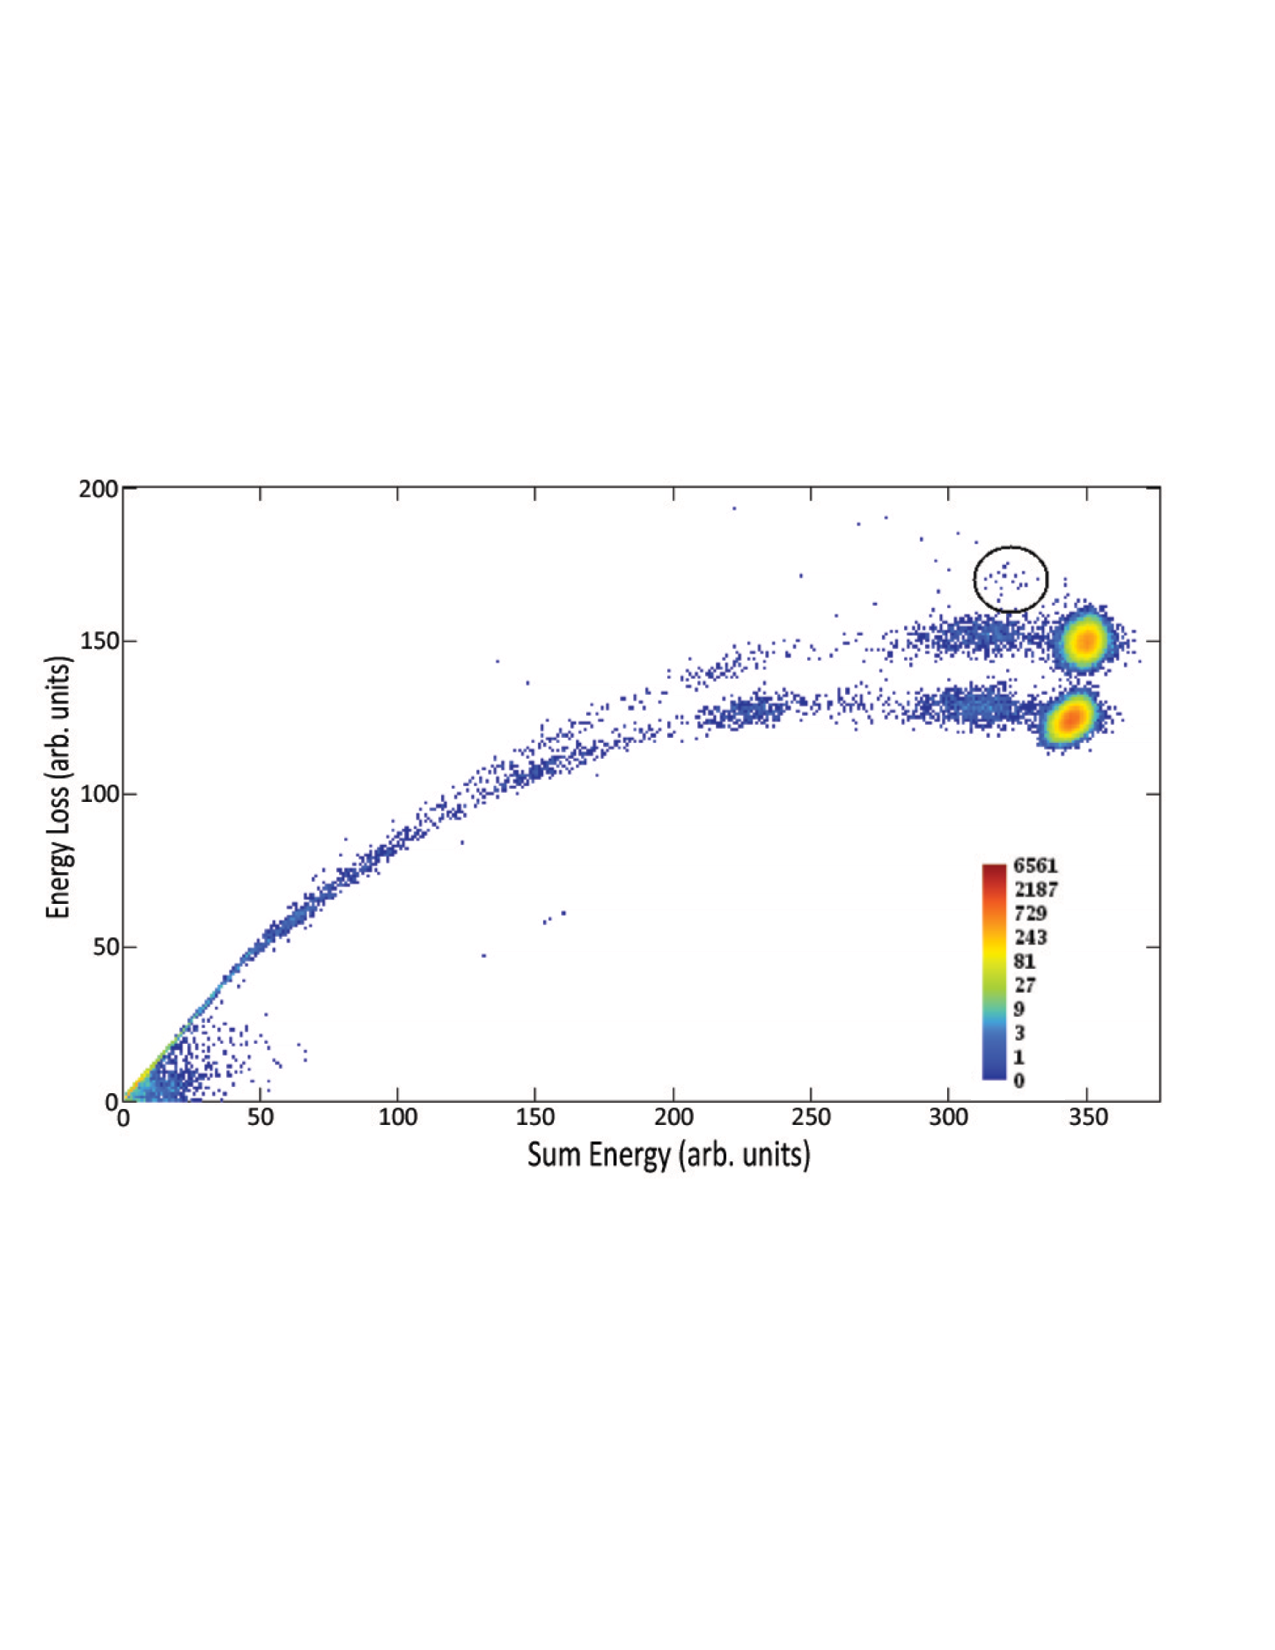
\includegraphics{chipps_fig06}
}
%\vspace{5cm}       % Give the correct figure height in cm
\caption{Energy loss versus total energy from the ionization chamber for the 599.8 keV resonance; \nuc{18}{Ne} recoils are indicated by the black circle. Taken from \cite{chip09a}.}
\label{fig:chipp09a_3}
\end{center}
\end{figure*}
Given the amount of background visible, this experiment, yielding an $\omega\gamma \approx 30 \unit{meV}$, was clearly showing the limits of the sensitivity of the DRS setup. Further improvements would be possible through the addition of a $\gamma$ array around the target to allow coincidence measurements and efforts to further suppress the leaky beam components transmitted to the focal plane.

\subsection{\nuc{23}{Mg}\reac{p}{\gamma}\nuc{24}{Al} (DRAGON)}
The \nuc{23}{Mg}\reac{p}{\gamma}\nuc{24}{Al} is another which affects the ejected abundance of $^{22}$Na (and to a lesser extent, $^{26g}$Al) in O-Ne-Mg novae \cite{ili02}, though the large variation came mainly from the large uncertainty in the rate rather than the sensitivity of the $^{22}$Na yields to small variations in the rate. This large uncertainty stemmed mainly from the absence of direct measurements of the reaction and sparse indirect experimental information concerning the states in $^{24}$Al, mainly from the $^{24}$Mg($^{3}$He,t)$^{24}$Al reaction \cite{gre91,kub95,vis07,zeg08} and a $\gamma$-decay study using $^{10}$B($^{16}$O,2n$\gamma$)$^{24}$Al \cite{lot08}. 
The first direct measurement of the \nuc{23}{Mg}\reac{p}{\gamma}\nuc{24}{Al} reaction, in particular the $E_{R}=486$ keV dominant resonance at nova temperatures, was performed at the DRAGON facility \cite{eri10}. The $^{23}$Mg was produced using a high-power silicon carbide target at ISAC, and resonantly ionized using the ISAC laser ion source \cite{las09}. This resulted in an accelerated beam of mixed $^{23}$Na and $^{23}$Mg, with the peak $^{23}$Mg current of around $3\times10^{7}$ s$^{-1}$. The ratio $^{23}$Na:$^{23}$Mg was time-varying and ranged between (20:1 -- 1000:1). This presented the challenge of not only of determining the $^{23}$Mg integrated flux over the duration of the experiment, but also separating leaky A=23 beam components (both Na and Mg) from both $^{24}$Al and $^{24}$Mg recoils (the latter from \nuc{23}{Na}\reac{p}{\gamma}\nuc{24}{Mg}). This was done using a combination of local time-of-flight measurements by the DRAGON MCPs, $\Delta$E-E measurements in the multi-anode ionization detector, coincidence detection of particles with prompt $\gamma$-ray events in the BGO array, and separator time-of-flight. Figures \ref{fig:Mg23_tof_IC} and \ref{fig:Mg23_dE_E} show some example data for one of the DRAGON \nuc{23}{Mg}\reac{p}{\gamma}\nuc{24}{Al} runs. Checks were also performed by eliminating the $^{23}$Mg by switching off the laser ionization, to determine the extend of the $^{23}$Na-induced background.  
Due to an uncertainty in the true resonance energy, BGO hit pattern data indicated that the reactions were occurring upstream in the DRAGON extended gas target, rather than in the centre where expected given the adopted resonance energy of $E_{R}=473$ keV that was accepted before the experiment. Because it could not be certain that the reactions were occurring in plateau region of gas density in the target, a 2D probability distribution in the resonance strength ($\omega\gamma$) and resonance energy ($E_{R}$) variables could only be constructed, leading to extracted values of $E_{R}=485.7^{+1.3}_{1.8}$ keV and $\omega\gamma=38^{+21}_{-15}$ meV, with the central values and uncertainties taken as the medians and 16\% and 84\% quartiles of the 2D PDF. 
A re-evaluation of old measurements in the literature of the $^{24}$Al mass excess, combined with the $\gamma$-ray measurements of \cite{lot08} presented in the DRAGON work \cite{eri10}, also suggested that $E_{R}=480(6)$ keV (uncertainties at 1$\sigma$).     
A subsequent mass measurement \cite{wre10} of $^{24}$Al enabled a new determination of $E_{R}$, which was combined with the DRAGON results to result in adopted values of $E_{R}=484.3^{+1.3}_{1.7}$ keV and $\omega\gamma=26^{+15.4}_{-7.0}$ meV.
These results drastically reduce the uncertainty of the \nuc{23}{Mg}\reac{p}{\gamma}\nuc{24}{Al} rate to a level sufficient for nucleosynthetic calculations of O-Ne-Mg novae. The experiment represented an original challenge for a recoil separator when the RIB was embedded in a stable isobar component of much higher intensity. 

\begin{figure}
\begin{center}
\resizebox{1.0\columnwidth}{!}{
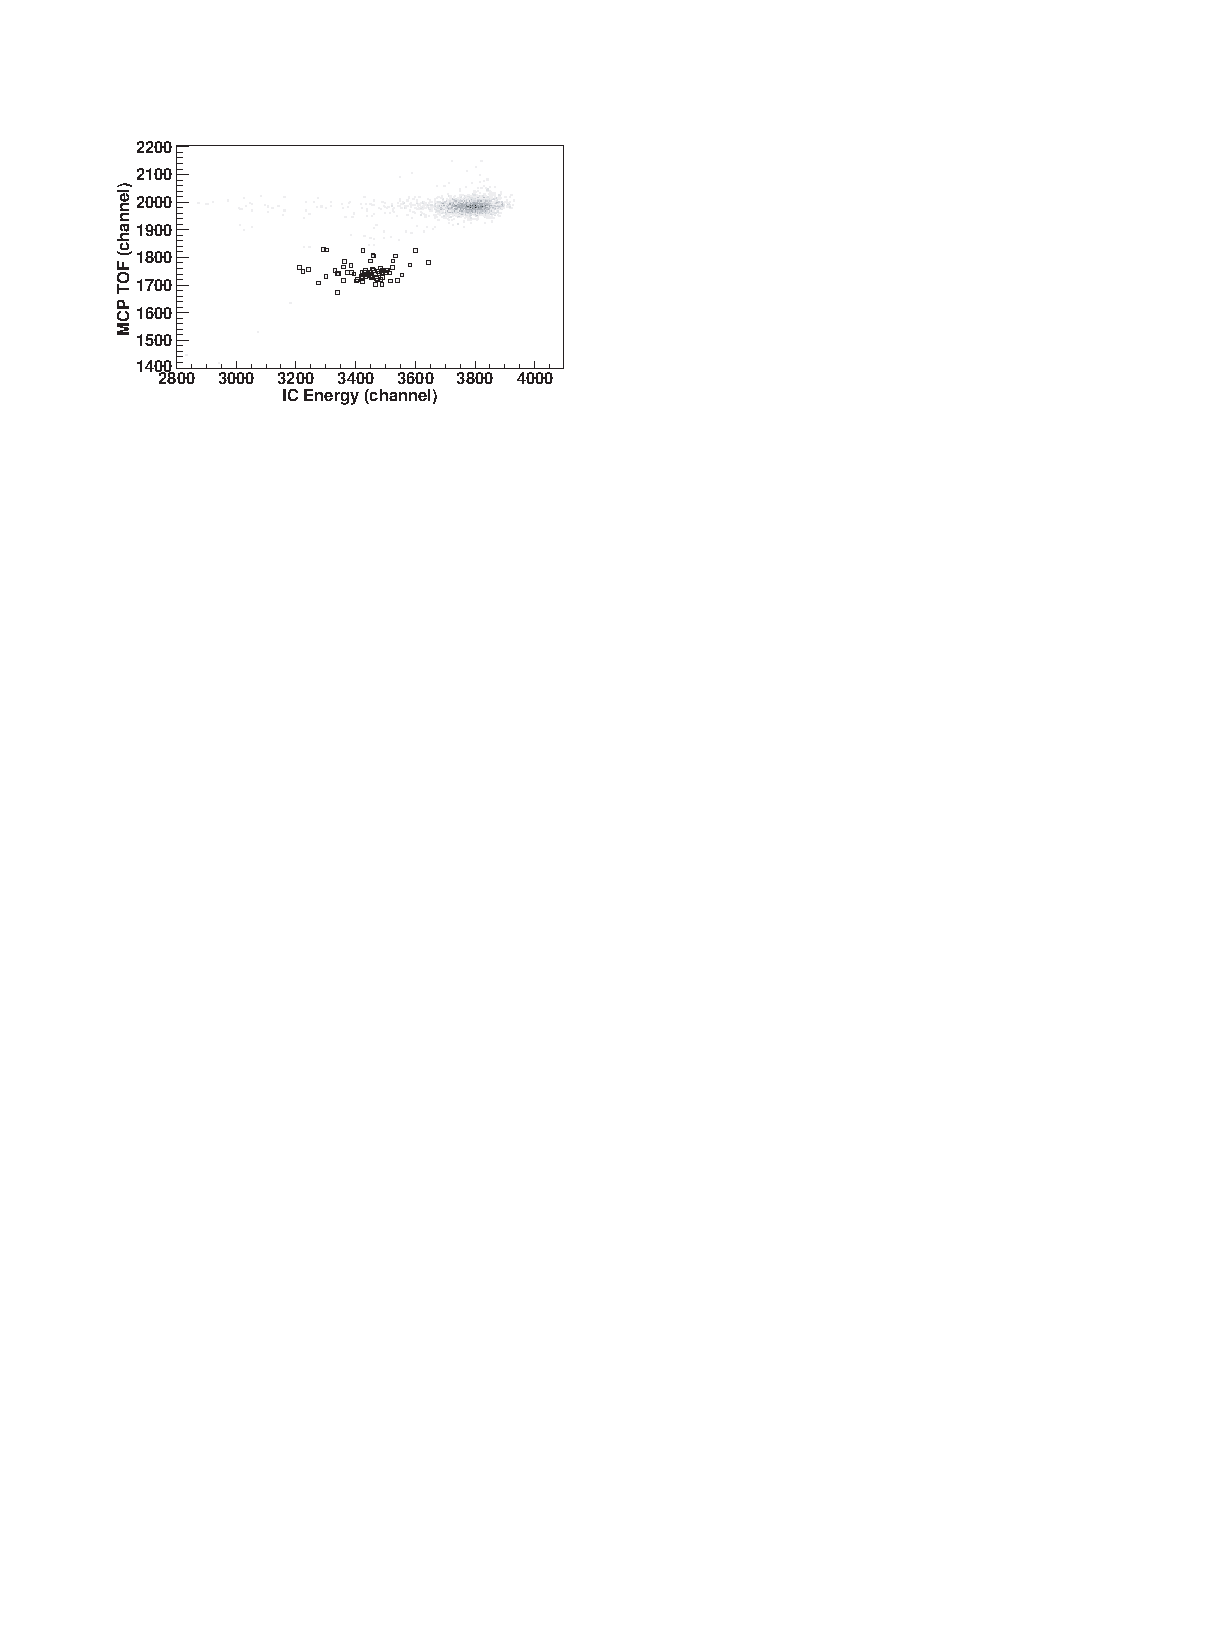
\includegraphics{Mg23_tof_IC}
}
\caption{Local time-of-flight vs. total detected energy for `singles' (not coincident with a prompt $\gamma$ ray) recoil events for the DRAGON \nuc{23}{Mg}\reac{p}{\gamma}\nuc{24}{Al} measurement. The grey density plot indicates all detected particles, while the open squares indicate A=24 recoils, clearly showing separation between `leaky' A=23 beam and A=24 recoils. Taken from \cite{eri10}.}
\label{fig:Mg23_tof_IC}
\end{center}
\end{figure}

\begin{figure}
\begin{center}
\resizebox{1.0\columnwidth}{!}{
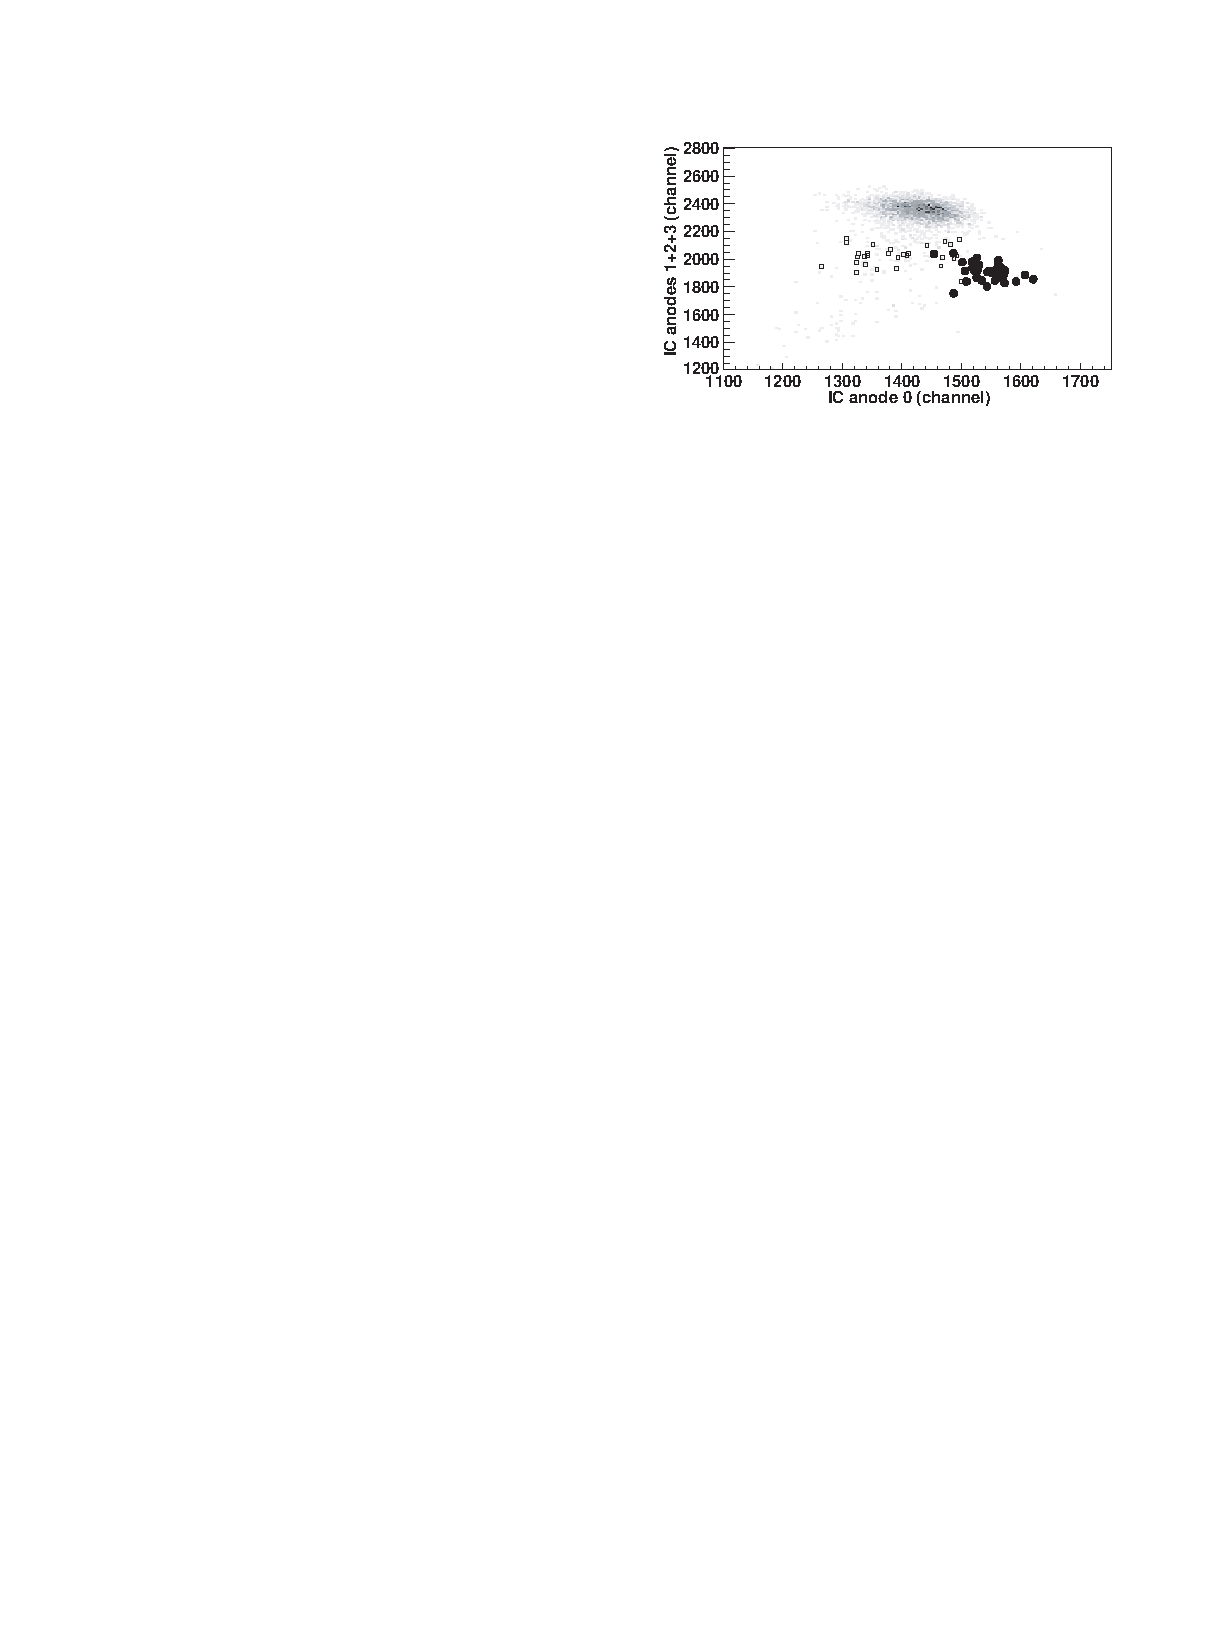
\includegraphics{Mg23_dE_E}
}
\caption{$\Delta$E vs. E for singles events in the DRAGON \nuc{23}{Mg}\reac{p}{\gamma}\nuc{24}{Al} measurement. The grey density plot indicates all detected particles. The open squares indicate all A=24 recoils, while the black circles indicate $^{24}$Al recoils. Taken from \cite{eri10}.}
\label{fig:Mg23_dE_E}
\end{center}
\end{figure}

\begin{figure}
\begin{center}
\resizebox{1.0\columnwidth}{!}{
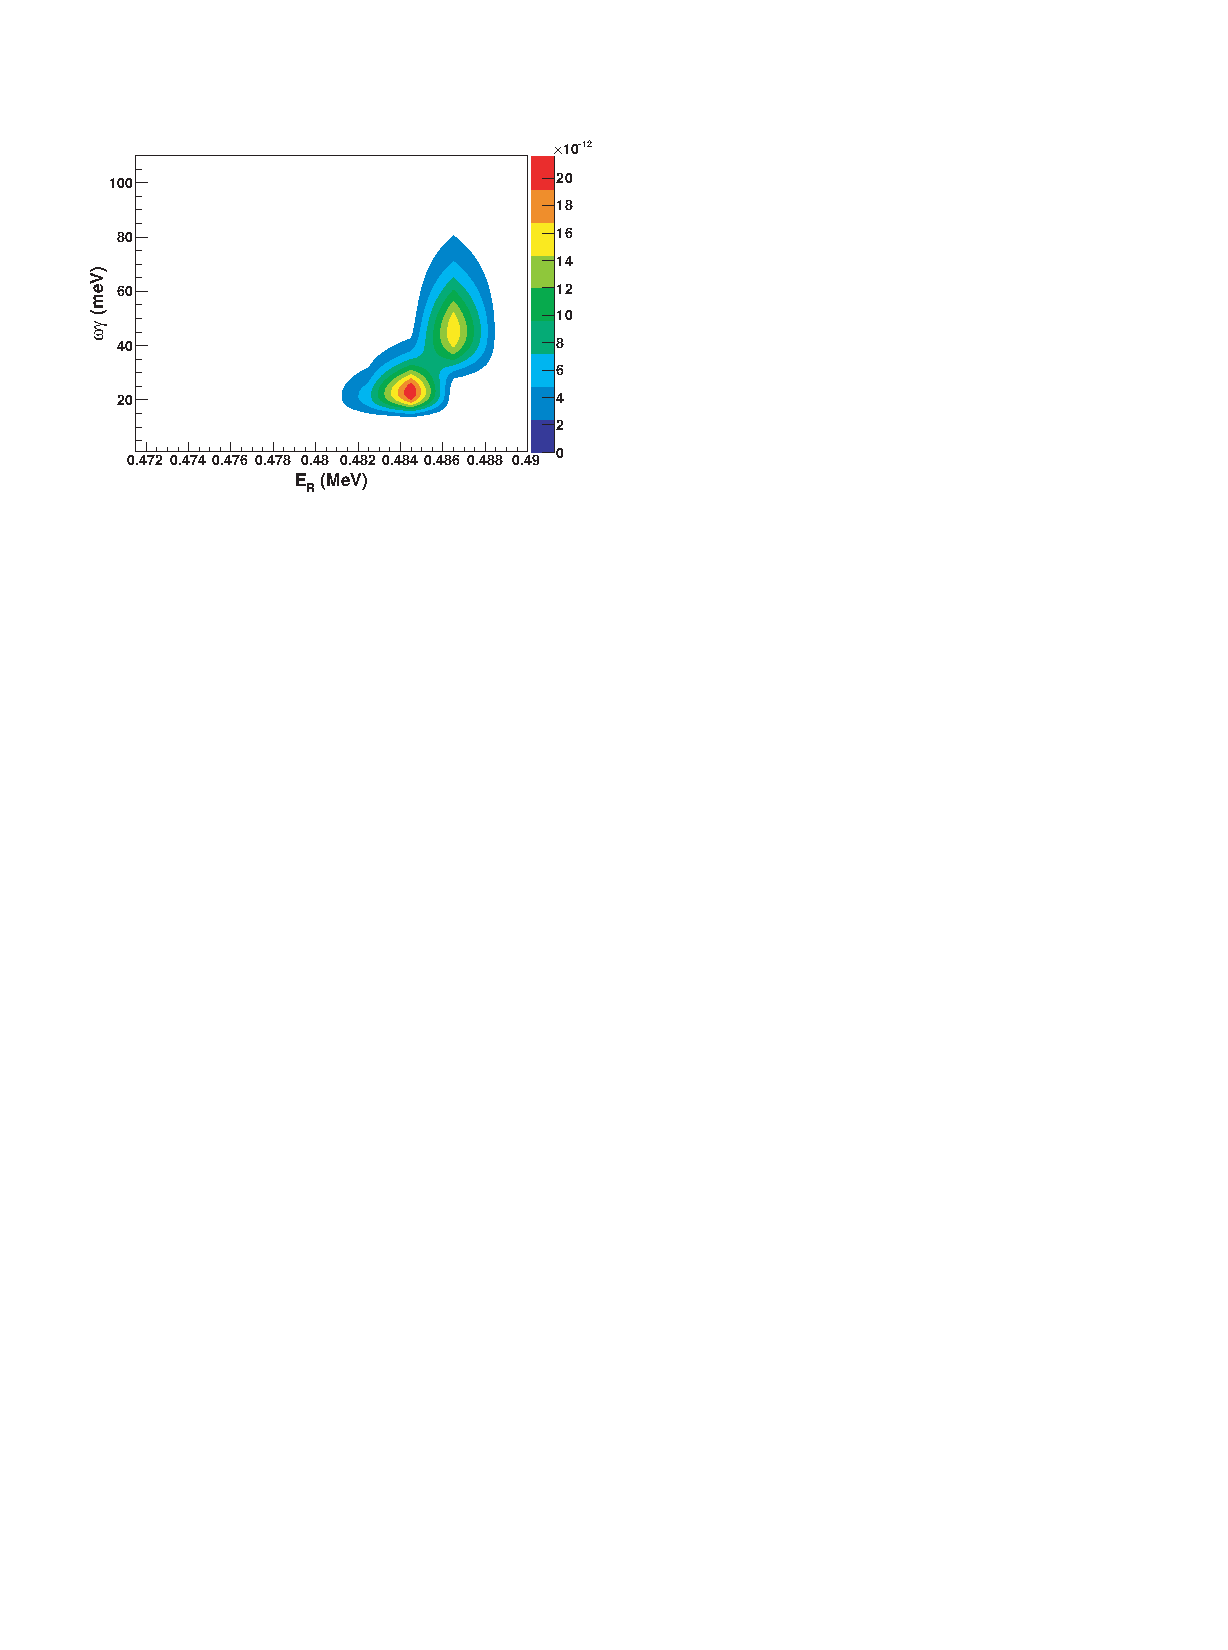
\includegraphics{Erikson_2010}
}
\caption{Probability contours for the determination of resonance strength, $\omega\gamma$, and resonance energy $E_{R}$, from the DRAGON measurement of \nuc{23}{Mg}\reac{p}{\gamma}\nuc{24}{Al}, taken from \cite{eri10}.}
\end{center}
\end{figure}      % Scientific highlights

\section{Outlook and guidance for future separators}

\subsection{Recoil separators planned and under construction}

At the time of writing, there are a handful of recoil separators being constructed or in the conceptual or design phase at laboratories worldwide. It is not the intention of the authors to summarize all of these proposals, as some of these may evolve in design, switch scientific focus, or indeed not be funded. However there are a couple of developments worth mentioning here, specifically projects that are aimed at astrophysics and are under detailed design or construction now. 

St. George (Strong Gradient Electromagnetic Online Recoil separator for capture Gamma Ray Experiments) \cite{cou08} is a recoil separator under construction at the Institute for Structure and Nuclear Astrophysics at the University of Notre Dame. The design is optimized for the study of astrophysical low energy ($\alpha,\gamma$) reactions for up to A=40 beam mass. The beams will be provided by the new 5MV accelerator at the laboratory. The separator has design acceptance values of $\pm$40 mrad in angle and $\pm$7.5\% in energy. It is built in a configuration providing selection of a single charge state via magnetic analysis, before mass separation is performed in a Wien filter (see figure \ref{fig:stgeorge}), with a final resolving power of $m/\Delta m=100$. It is designed to have high a beam suppression factor of $\ge10^{15}$. In particular the Wien filter element of this separator is specially optimized to improve the filtering efficiency, achieved by minimizing the magnetic dipole component fringe fields and by incorporating specially-shaped electrodes so that the electric fringe fields closely follow the magnetic ones. 

The Separator for Capture Reactions (SECAR) is a recoil separator design destined to be a flagship experiment at the Facility for Rare Isotope Beams (FRIB)  at the National Superconducting Cyclotron Laboratory (NSCL) at Michigan State University. The present design is based on the St. George separator, but using an additional Wien filter \cite{ber10}. The separator will operate using reaccelerated radioactive ion beams produced by fragmentation at FRIB and prepared using a gas stopper system. The scientific purpose of this experiment is to continue the study of proton- and alpha- induced radiative capture reactions for explosive nucleosynthesis and represents an important part of the US nuclear physics community's long range plan. The JENSA jet gas target mentioned in section \ref{gas} \cite{chi13} is planned for use with the SECAR separator. 

\begin{figure}
\resizebox{0.9\columnwidth}{!}{
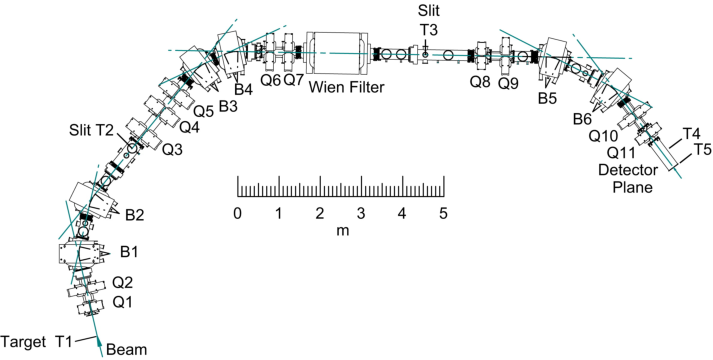
\includegraphics{stgeorge}
}
%\vspace{5cm}       % Give the correct figure height in cm
\caption{Schematic view of the St. George separator. Taken from \cite{cou08}.}
\label{fig:stgeorge}
\end{figure}



\subsection{Suggested avenues of technical development} 

\subsubsection{Acceptance}

\subsubsection{Rigidity}

\subsubsection{Operation}

\subsubsection{Detection}           % Outlook and guidance for future separators



%\bibliographystyle{aaalike}
\bibliographystyle{unsrt}
 \bibliography{refs}



\end{document}


